\protect\hypertarget{_Hlk129432535}{}{}4 ano

\section{1. Representar quantidades}\label{muxf3dulo-1}

\colorsec{Habilidades do SAEB}

\begin{itemize}
\item Escrever números racionais (naturais de até 6 ordens, representação
fracionária ou decimal finita até a ordem dos milésimos) em sua
representação por algarismos ou em língua materna ou associar o registro
numérico ao registro em língua materna.
\item Identificar a ordem ocupada por um algarismo ou seu valor posicional
(ou valor relativo) em um número natural de até 6 ordens.
\item Comparar ou ordenar números racionais (naturais de até 6 ordens,
representação fracionária ou decimal finita até a ordem dos milésimos),
com ou sem suporte da reta numérica.
\item Compor ou decompor números naturais de até 6 ordens na forma aditiva,
ou em suas ordens, ou em adições e multiplicações.
\item Comparar diferentes sentenças de adições ou de subtrações de dois
números naturais.
\item Determinar o número desconhecido que torna verdadeira uma igualdade
que envolve as operações fundamentais com números naturais de até 6
ordens.
\end{itemize}

\colorsec{Habilidades da BNCC}

\begin{itemize}
\item EF04MA01, EF04MA02.
\end{itemize}

\subsection{Conteúdo}\label{conteuxfado}
\Produzir uma tabela igual à de baixo utilizando padrão de cores que o material seguirá

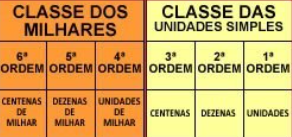
\includegraphics[width=3.55128in,height=1.66618in]{media/image1.png}

Valor posicional ou relativo: é o valor que o algarismo assume
dependendo da classe e da ordem em que ele está posicionado no número.

Exemplo: no número 352.146, o algarismo 5 apresenta valor posicional ou
relativo igual a 50.000, pois ocupa a 5º ordem, a qual está dentro da
classe dos milhares; ou seja, está na posição da dezena de milhar e,
sendo assim, 5 x 10.000 = 50.000.

Sistema de numeração Egípcio: era baseado em figuras; cada figura tinha um valor específico e a combinação entre figuras formava as qantidades e os valores que se desejava representar. 

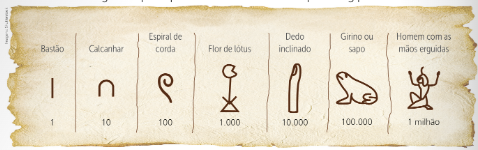
\includegraphics[width=3.98368in,height=1.25011in]{media/image2.png}

Sistema de numeração Maia: era baseado em representar
números com pontos e traços, conforme a figura.

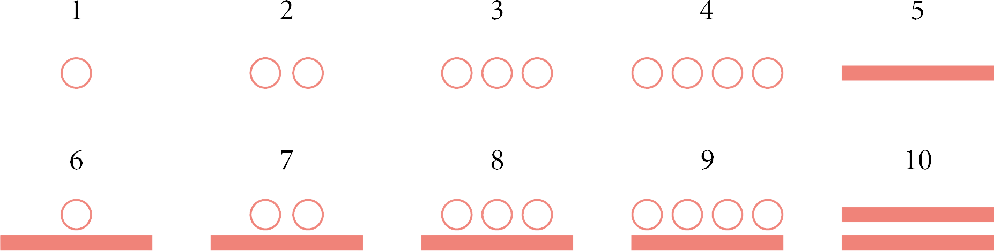
\includegraphics[width=2.66690in,height=0.81674in]{media/image3.png}

Sistema de numeração Romano: representava os números com letras
maiúsculas, seguindo regras específicas para essa representação.

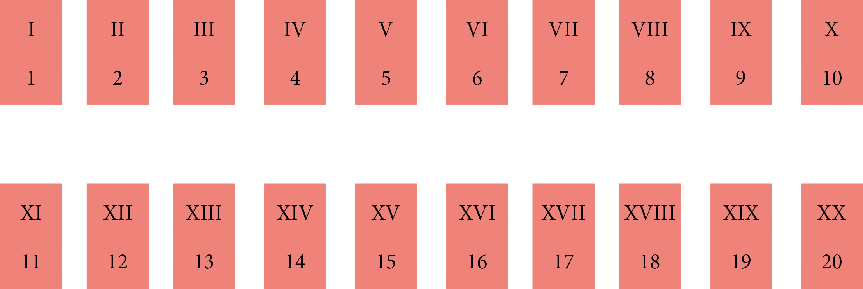
\includegraphics[width=3.97534in,height=1.23344in]{media/image4.png}

Sistema de numeração indo-arábico: é o utilizado por nós
até hoje e, com o passar do tempo, foi evoluindo na escrita dos algarismos e, consequentemente, dos números, como está representado na figura.

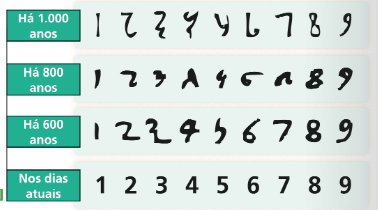
\includegraphics[width=3.15027in,height=1.75015in]{media/image5.png}

\subsection{Atividades}\label{atividades}

\subsubsection{1.}\label{section}

Escreva o valor posicional de cada algarismo
destacado -- ou seja, o valor que cada um assume de acordo com a posição
que ocupa no número.

\begin{enumerate}
\def\labelenumi{\alph{enumi})}
\item
  \textbf{8}24.345:
  Valor posicional do 8 nesse caso: 800.000 -- centena de milhar.
\item
  3\textbf{7}5.6\textbf{7}8:
  Valor posicional da primeira ocorrência do 7 nesse caso: 70.000 -- dezena de milhar.
  Valor posicional da segunda ocorrência do 7 nesse caso: 70 -- dezena comum.
\item
  14\textbf{8}.52\textbf{1}:
  Valor posicional do 8 nesse caso: 8.000 -- unidade de milhar.
  Valor posicional do 1 nesse caso: 1 -- unidade comum.

\subsubsection{2.}\label{section-1}

Decomponha os números a seguir de acordo com o valor posicional de cada
algarismo.

\begin{enumerate}
\def\labelenumi{\alph{enumi})}
\item
  32.084
\end{enumerate}

Deixar uma linha para resposta
30 000 + 2 000 + 80 + 4; 3 x 10 000 + 2 x 1 000 + 0 x 100 + 8 x 10 + 4.

\begin{enumerate}
\def\labelenumi{\alph{enumi})}
\item
  26.587
\end{enumerate}

Deixar uma linha para resposta
20 000 + 6 000 + 500 + 80 + 7; 2 x 10 000 + 6 x 1 000 + 5 x 100 + 8
  x 10 + 7.
\item
  
\begin{enumerate}
\def\labelenumi{\alph{enumi})}
\item
  2.105
\end{enumerate}

Deixar uma linha para resposta
2 000 + 100 + 5; 2 x 1 000 + 1 x 100 + 0 x 10 + 5


\subsubsection{3.}\label{section-2}

Monte os número compostos e registre-os nas linhas a seguir.

\begin{enumerate}
\def\labelenumi{\alph{enumi})}
\item
  7 unidades de milhar, 5 centenas e 4 unidades.
\end{enumerate}

deixar uma linha aqui na frente para resposta
7.504.

\begin{enumerate}
\def\labelenumi{\alph{enumi})}
\item
  3 dezenas de milhar, 7 dezenas e 2 unidades:
\end{enumerate}

deixar uma linha aqui na frente para resposta
30.072.

\begin{enumerate}
\def\labelenumi{\alph{enumi})}
\item
  9 centenas de milhar, 5 unidades de milhar e 6 centenas:
\end{enumerate}

deixar uma linha aqui na frente para resposta
905.600.

\begin{enumerate}
\def\labelenumi{\alph{enumi})}
\item
  2 unidades de milhar, 6 centenas e 3 unidades:
\end{enumerate}

deixar uma linha aqui na frente para resposta
2.603

É necessário explorar bem a montagem dos números, pois muitos alunos sabem fazer a decomposição, mas não compreendem a volta.

\subsubsection{4.}\label{section-3}

Ligue um número da coluna da esquerda com a forma escrita correspondente na coluna da direita.

352.700 Trezentos e quatorze mil

200.015 Vinte mil e três

20.003 Trezentos e cinquenta e dois mil e setecentos

314.000 Duzentos mil e quinze

Resposta:

352 700 deve estar ligado ao trezentos e cinquenta e dois mil e
setecentos.

200 015 deve estar ligado ao duzentos mil e quinze.

20 003 deve estar ligado a vinte mil e três.

314 000 deve estar ligado ao trezentos e quatorze mil.

\subsubsection{5.}\label{section-4}

Monte um número a partir de cada composição a seguir e escreva-o por extenso.

\begin{escolha}
\def\labelenumi{\alph{enumi})}
\item 5 x 100 + 4 x 10 + 5 x 1
545.
\item 3 x 1.000 + 0 x 100 + 9 x 10 + 3 x 1
3.093.
\item 4 x 10.000 + 8 x 1.000 + 5 x 100 + 0 x 10 + 2 x 1
48.502.
\item 3 x 100.000 + 1 x 10.000 + 6 x 1.000 + 2 x 100 + 1 x 10 + 3 x 1
316.213.
\end{escolha}

\subsubsection{6.}\label{section-5}

Escreva por extenso cada um dos números montados na atividade anterior.

Deixar 8 linhas para resposta
Quinhentos e quarenta e cinco.

Três mil e noventa e três.

Quarenta e oito mil quinhentos e dois.

Trezentos e dezesseis mil duzentos e treze.

\subsubsection{7.}\label{section-6}

Observe os números no quadro a seguir e relacione cada um a uma característica.

147.254 -- 464.823 -- 9.998 -- 99.999

O maior número com exatamente 5 ordens.
99.999.

O segundo maior número formado por 4 ordens.
9.998.

Um número ímpar com 6 ordens.
464 823.

Um número de 6 ordens com algarismo da unidade de milhar igual a 7.
147.254.


\subsubsection{8.}\label{section-7}

Represente os números a seguir utilizando os símbolos maias.

\begin{enumerate}
\def\labelenumi{\alph{enumi})}
\item
  11
\end{enumerate}

Deixar um retângulo para resposta.
O aluno deve usar duas linhas e um ponto.

\begin{enumerate}
\def\labelenumi{\alph{enumi})}
\item
  12
\end{enumerate}

Deixar um retângulo para resposta.
O aluno deve usar duas linhas e dois pontos.

\begin{enumerate}
\def\labelenumi{\alph{enumi})}
\item
  13
\end{enumerate}

Deixar um retângulo para resposta.
O aluno deve usar duas linhas e três pontos.

\begin{enumerate}
\def\labelenumi{\alph{enumi})}
\item
  14
\end{enumerate}

Deixar um retângulo para resposta.
O aluno deve usar duas linhas e quatro pontos.

\begin{enumerate}
\def\labelenumi{\alph{enumi})}
\item
  15
\end{enumerate}

Deixar um retângulo para resposta.
O aluno deve usar duas linhas seguidas de uma linha.

\begin{enumerate}
\def\labelenumi{\alph{enumi})}
\item
  16
\end{enumerate}

Deixar um retângulo para resposta.
O aluno deve usar duas linhas seguidas de um ponto sobre uma linha.

\begin{enumerate}
\def\labelenumi{\alph{enumi})}
\item
  17
\end{enumerate}

Deixar um retângulo para resposta.
O aluno deve usar duas linhas seguidas de dois pontos sobre uma linha.

\begin{enumerate}
\def\labelenumi{\alph{enumi})}
\item
  18
\end{enumerate}

Deixar um retângulo para resposta.
O aluno deve usar duas linhas seguidas de três pontos sobre uma linha.

\begin{enumerate}
\def\labelenumi{\alph{enumi})}
\item
  19
\end{enumerate}

Deixar um retângulo para resposta.
O aluno deve usar duas linhas seguidas de quatro pontos sobre uma linha.


\subsubsection{9.}\label{section-8}

Escreva cada um dos números a seguir utilizando o sistema indo-arábico.

\begin{enumerate}
\def\labelenumi{\alph{enumi})}
\item
  Dois mil trezentos e cinco.\_\_\_\_\_\_\_\_\_\_\_\_\_
\item
  Quinze mil e quarenta e sete.\_\_\_\_\_\_\_\_\_\_\_\_\_
\item
  Vinte mil e novecentos.\_\_\_\_\_\_\_\_\_\_\_\_\_\_
\item
  Trinta e três mil trezentos e trinta e três.\_\_\_\_\_\_\_\_\_\_\_\_\_
\item
  Cinquenta mil e cinco.\_\_\_\_\_\_\_\_\_\_\_\_\_\_\_\_\_\_\_\_
\end{enumerate}

Resposta:

\begin{enumerate}
\def\labelenumi{\alph{enumi})}
\item
  2.305
\item
  15.047
\item
  20.900
\item
  33.333
\item
  50.005
\end{enumerate}

\subsubsection{10.}\label{section-9}

A bolas representadas a seguir fazem parte de um jogo conhecido como
bilhar ou como sinuca.

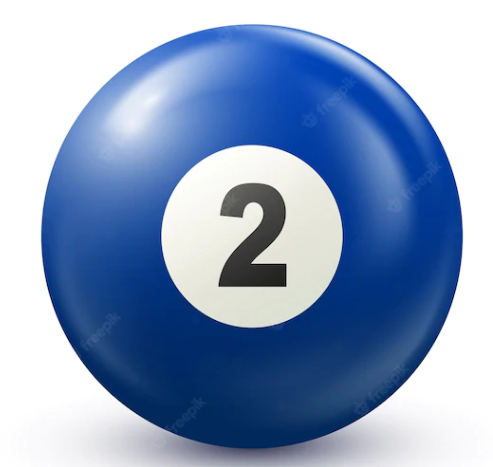
\includegraphics[width=1.40833in,height=1.33406in]{media/image21.png}

\url{https://img.freepik.com/vetores-premium/bola-de-bilhar-azul-com-numero-2-snooker-ou-bola-de-loteria-em-fundo-branco-ilustracao_390775-925.jpg?w=740}

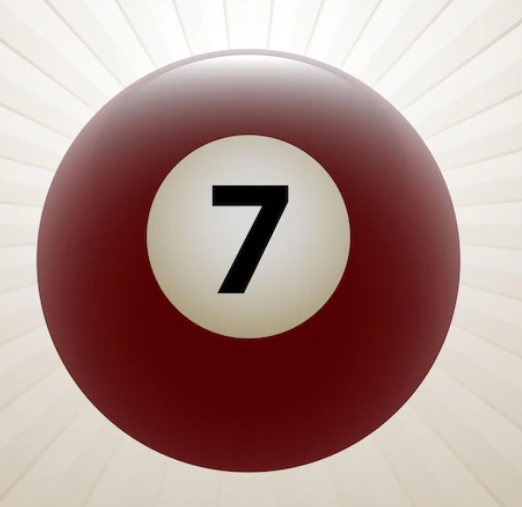
\includegraphics[width=1.66667in,height=1.61877in]{media/image22.png}

\url{https://img.freepik.com/vetores-premium/bilhar_672017-1383.jpg?w=740}


\includegraphics[width=1.68333in,height=1.36449in]{media/image23.png}

\url{https://img.freepik.com/psd-premium/ilustracao-3d-da-bola-de-bilhar-oito_446709-517.jpg?w=740}

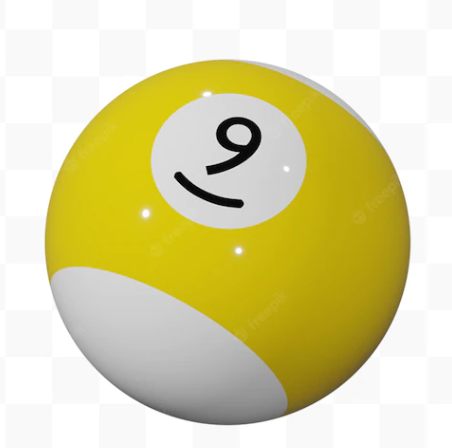
\includegraphics[width=1.61667in,height=1.60236in]{media/image24.png}

\url{https://img.freepik.com/psd-premium/bola-de-bilhar-3d-numero-9_592419-130.jpg?w=740}

Colocar as bolinhas na mesma linha

Observando os números representados em cada bola, responda ao que se pergunta a seguir.

\begin{enumerate}
\def\labelenumi{\alph{enumi})}
\item
  Qual é o menor número entre essas bolas?
  2 (dois).
\item
  Qual é o menor número com exatamente 4 ordens que podemos formar com essas bolas?
  2.789 (dois mil setecentos e oitenta e nove).
\item
  Qual é o maior número par que podemos formar com essas bolas?
  9.872 (nove mil oitocentos e setenta e dois).
\end{enumerate}

Explore mais exemplos com os alunos para estimular a formação de números
e a criatividade de cada um deles.

\subsection{Treino}\label{treino}

\subsubsection{1.}\label{section-10}

Amanda estava brincando no escritório de seu pai quando encontrou um
pedaço de papel em que estava escrito isto:

Faturamento semestral: R\$ 650.734,00.

Lembrando-se das aulas de Matemática, a menina resolveu decompor o número escrito
no papel. Qual é a decomposição correta que Amanda poderá fazer desse
número?

\begin{enumerate}
\def\labelenumi{\alph{enumi})}
\item
  600.000 + 50.000 + 700 + 30 + 4.
\item
  600.000 + 5.000 + 70 + 3 + 4.
\item
  600.000 + 500 + 700 + 30 + 4.
\item
  60.000 + 50.000 + 70 + 300 + 4.
\end{enumerate}

SAEB: Compor ou decompor números naturais de até 6 ordens na forma aditiva, ou em suas ordens, ou em adições e multiplicações.
BNCC: EF04MA02 -- Mostrar, por decomposição e composição, que todo número natural pode ser escrito
por meio de adições e multiplicações por potências de dez, para compreender o sistema de
numeração decimal e desenvolver estratégias de cálculo.

a) Correta. Todas as ordens estão corretamente representadas e somadas entre si.
b) Incorreta. As quantidades indicadas pelos algarismos 5, 7 e 3 estão erradas.
c) Incorreta. As quantidades indicadas pelos algarismos 5 e 7 estão erradas.
d) Incorreta. As quantidades indicadas pelos algarismos 7 e 3 estão erradas.


\subsubsection{2.}\label{section-11}

Vpitor escreveu o seguinte número utilizando os algarismos romanos:

XIX

Esse número, no sistema indo-arábico, é o:

\begin{enumerate}
\def\labelenumi{\alph{enumi})}
\item
  9.
\item
  19.
\item
  21.
\item
  11.
\end{enumerate}

SAEB: Escrever números racionais (naturais de até 6 ordens, representação fracionária ou decimal finita até a ordem dos milésimos) em sua representação por algarismos ou em língua materna ou associar o registro numérico ao registro em língua materna.
BNCC: EF04MA01 -- Ler, escrever e ordenar números naturais até a ordem de dezenas de milhar.

a)  Incorreta. Faltou considerar o valor do primeiro X.
b)  Correta. O número formado pelas duas últimas letras (IX), 9, deve ser somado ao número representado pela primeira letra (X), 10: 10 + 9 = 19.
c)  Incorreta. Dessa forma, não se leva em consideração a ordem da escrita.
d)  Incorreta. Faltou considerar o valor do segundo X.


\subsubsection{3.}\label{section-12}

José resolveu comprar uma placa com o número de sua casa. Observe a seguir.

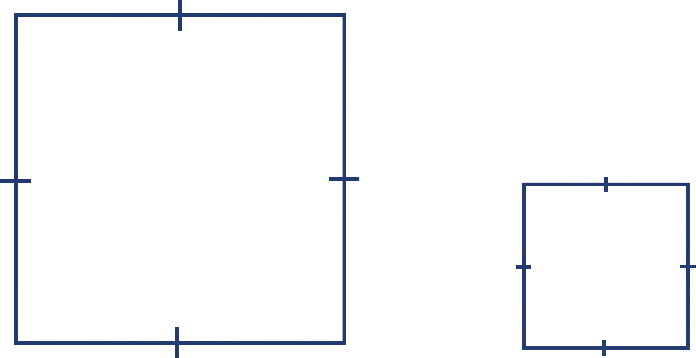
\includegraphics[width=3.02500in,height=1.48973in]{media/image26.png}

\url{https://img.freepik.com/fotos-gratis/numero-125_1122-1156.jpg?w=1060\&t=st=1677434865~exp=1677435465~hmac=526ac25f92ac28e692177f84842345ca95b5e246e04ca35259750459c4f3e954}

Depois, percebeu que o número estava
errado, já que o primeiro e o último algarismo estão nas posições
trocadas. Qual é o valor relativo do último algarismo no lugar em que ele se
encontra na placa errada e qual deveria ser seu valor relativo no número
correto da casa de José?

\begin{enumerate}
\def\labelenumi{\alph{enumi})}
\item
  Está como 5 e deveria ser como 50.
\item
  Está como 50 e deveria ser como 500.
\item
  Está como 5 e deveria ser como 500.
\item
  Está como 50 e deveria ser como 5.
\end{enumerate}

SAEB: Identificar a ordem ocupada por um algarismo ou seu valor posicional (ou valor relativo) em um número natural de até 6 ordens.
BNCC: EF04MA01 -- Ler, escrever e ordenar números naturais até a ordem de dezenas de milhar.

a)  Incorreta. A identificação do valor na placa está correta, mas ele deveria estar como 500.
b)  Incorreta. O valor na placa deveria ser como 500, mas ele está como 5.
c)  Correta. Na placa, está representado o número 125 -- em que o algarismo 5 ocupa a ordem das unidades. O número representado deveria ser o 521 -- em que o algarismo 5 ocuparia a ordem das centenas.
d)  Incorreta. As duas identificações estão incorretas.


\section{2. As operações básicas}\label{muxf3dulo-2}

\colorsec{Habilidades do SAEB}

\begin{itemize}
\item Calcular o resultado de adições ou subtrações envolvendo números
naturais de até 6 ordens.
\item Calcular o resultado de multiplicações ou divisões envolvendo números
naturais de até 6 ordens.
\item Associar o quociente de uma divisão com resto zero de um número
natural de até 6 ordens por 2, 3, 4, 5 e 10 às ideias de metade, terça,
quarta, quinta e décima parte.
\item Resolver problemas de adição ou de subtração, envolvendo números
naturais de até 6 ordens, com os significados de juntar, acrescentar,
separar, retirar, comparar ou completar.
\item Resolver problemas de multiplicação ou de divisão, envolvendo números
naturais de até 6ordens, com os significados de formação de grupos
iguais (incluindo repartição equitativa e medida), proporcionalidade ou
disposição retangular.
\end{itemize}

\colorsec{Habilidade da BNCC}

\begin{itemize}
\item EF04MA07.
\end{itemize}

\subsection{Conteúdo}\label{conteuxfado-1}

\protect\hypertarget{_Hlk128407586}{}{}
\textbf{Adição}

Fazer a imagem abaixo segundo os padrões do projeto.

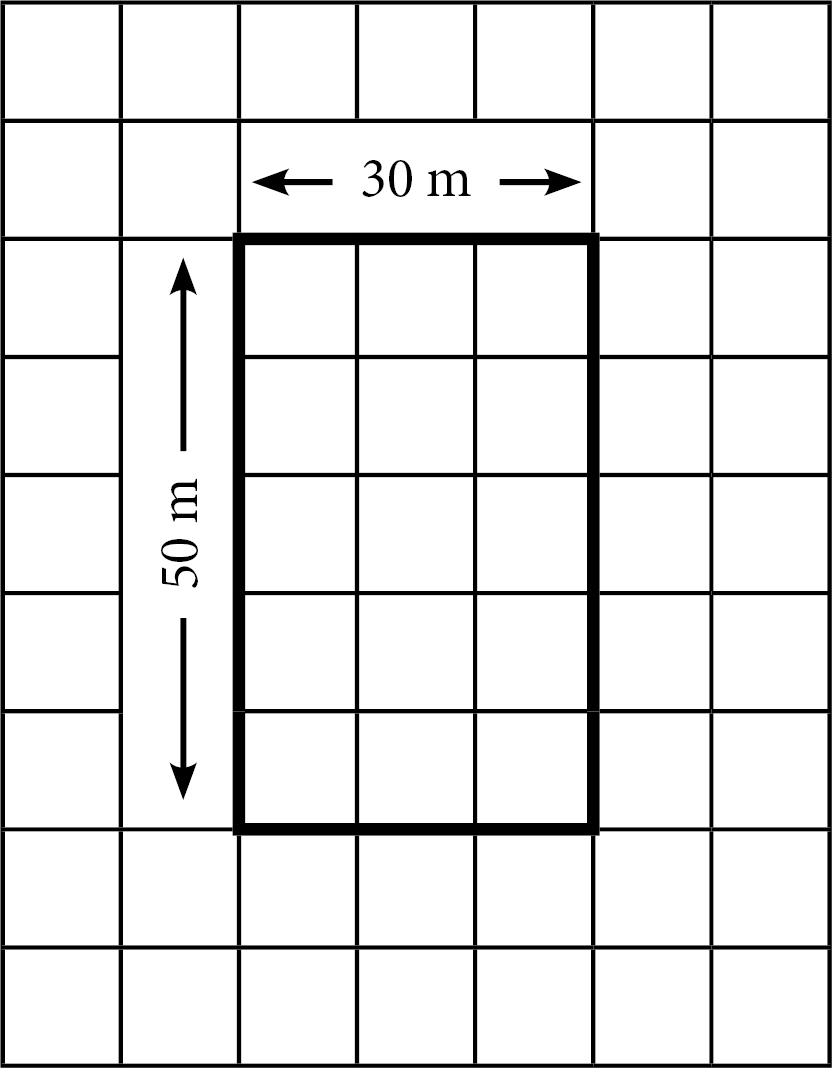
\includegraphics[width=2.26282in,height=1.19473in]{media/image27.png}

\textbf{Subtração}

Fazer a imagem abaixo segundo os padrões do projeto.

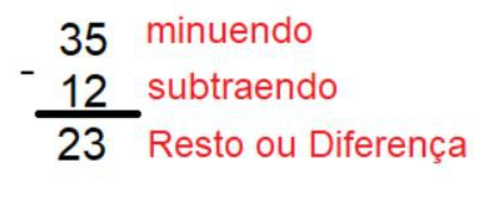
\includegraphics[width=2.55128in,height=1.04961in]{media/image28.png}

\textbf{Multiplicação}

Fazer a imagem abaixo segundo os padrões do projeto.

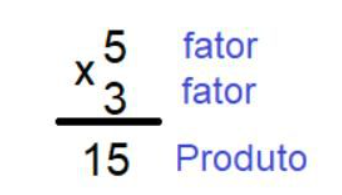
\includegraphics[width=1.92308in,height=1.09649in]{media/image30.png}

\textbf{Divisão}

Fazer a imagem abaixo segundo os padrões do projeto.

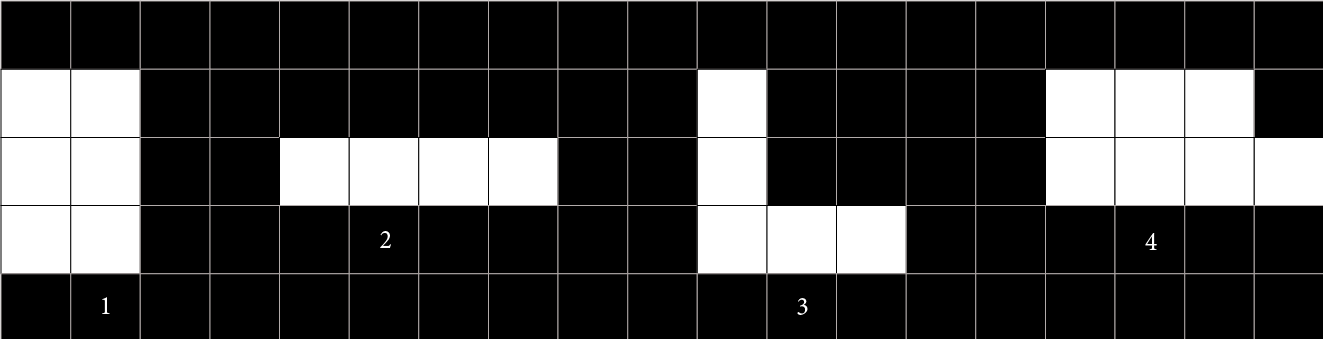
\includegraphics[width=2.26923in,height=1.66995in]{media/image31.png}

\subsection{Atividades}\label{atividades-1}

\subsubsection{1.}\label{section-13}

Ligue cada operação da coluna da esquerda com o resultado correto na
coluna da direita.

\ColunaDaEsquerda
584 -- 249

960 -- 723

767 -- 158

50 -- 2 x (5 + 15) + 2 x 3 -- 2 x 2) + 3 x (10 -- 4 x 2)

2 + 8 x 2 -- 2(1 + 2 x 3)

50 -- {[}24 + 3 x (2 + 3 x 2{]}

2 x 3 -- {[}10 -- 2 x (1 + 1 x 3){]}

\ColunaDaDireita
237
609
335
4
6
18
2

Deixar um retângulo em branco referente a 10 linhas para os alunos
efetuarem os cálculos necessários

\subsubsection{2.}\label{section-14}

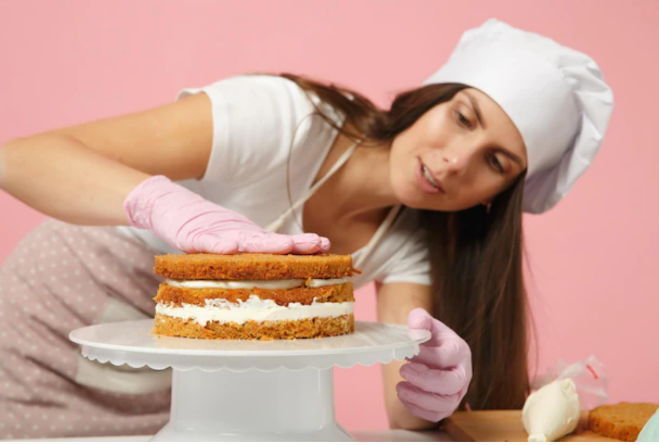
\includegraphics[width=3.00000in,height=2.02528in]{media/image32.png}

Segunda a receita de um bolo, devem-se inicialmente colocar 260 g de farinha
de trigo e misturar com outros ingredientes como ovos, açúcar e leite.
Em seguida, devem-se colocar mais 135 g de farinha de trigo para a massa
ficar no ponto ideal. Qual é a quantidade total de farinha, em quilogramas,
utilizada nessa receita?

https://img.freepik.com/fotos-premium/chef-cozinheiro-confeiteiro-ou-padeiro-em-t-shirt-branca-toque-chefs-chapeu-cozinhando-na-mesa-isolada-em-fundo-rosa-pastel-em-estudio-aplicacao-de-creme-processo-de-confeccao-de-bolos-mock-up-conceito-de-comida-de-espaco-de-copia\_365776-27137.jpg?w=1060

Deixar espaço em branco de 3 linhas para a resolução

Resposta:

260 + 135 = 395 g = 0,395 kg

\subsubsection{3.}\label{section-15}

A tabela a seguir mostra a população do Amapá dividida em municípios, segundo estimativa do IBGE de 2018.

\begin{longtable}[]{@{}ll@{}}
\toprule
Município & População estimada\tabularnewline
\midrule
\endhead
Macapá (capital) & 503.907\tabularnewline
Santana & 122.988\tabularnewline
Laranjal do Jari & 55.021\tabularnewline
Oiapoque & 29.563\tabularnewline
Mazagão & 27.436\tabularnewline
Porto Grande & 22.286\tabularnewline
Tartarugalzinho & 17.206\tabularnewline
Pedra Branca do Amapari & 16.624\tabularnewline
Vitória do Jari & 15.632\tabularnewline
Calçoene & 12.165\tabularnewline
Amapá & 10.842\tabularnewline
Ferreira Gomes & 9.373\tabularnewline
Cutias & 7.816\tabularnewline
Itaubal & 6.400\tabularnewline
Serra do Navio & 6.301\tabularnewline
Pracuuba & 5.632\tabularnewline
\bottomrule
\end{longtable}

A somatória das populações dos municípios sem contar a capital é maior ou menor que a população de Macapá? Justifique sua resposta com cálculos.

Deixar espaço de 5 linhas para cálculos

Resposta:

122.988 + 55.021 + 29.563 + 27.436 + 22.286 + 17.206 + 16.624 + 15.632 + 12.165 + 10.842 + 9.373 + 7.816 + 6.400 + 6.301 + 5.632 = 365.285 (menor que a população da capital, que é de 503.907).

Portanto a soma das populações estimadas dos municípios apresentados na
tabela, exceto São Paulo, é menor que a população da cidade de São
Paulo.

\subsubsection{4.}\label{section-16}

Faça o que se pede a seguir.

\begin{enumerate}
\def\labelenumi{\alph{enumi})}
\item
  Se em uma caixa cabem 1.000 bolinhas de gude de mesmo tamanho, quantas
  caixas precisaremos para guardar 6.536 bolinhas de gude desse mesmo
  tamanho?
\end{enumerate}

Deixar espaço em branco equivalente a 3 linhas para a resolução

\begin{enumerate}
\def\labelenumi{\alph{enumi})}
\item
  Se na caixa couberem apenas 100 bolinhas de gude de mesmo tamanho, quantas
  caixas serão necessárias para armazenar essas mesmas 6.536 bolinhas?
\end{enumerate}

Deixar espaço em branco equivalente a 3 linhas para a resolução

\begin{enumerate}
\def\labelenumi{\alph{enumi})}
\item
  Se a caixa só puder armazenar 10 bolinhas de mesmo tamanho, quantas caixas dessas
  serão necessárias para armazenar as mesmas 6.536 bolinhas de gude?
\end{enumerate}

Deixar espaço em branco equivalente a 3 linhas para a resolução

Resposta:

\begin{enumerate}
\def\labelenumi{\alph{enumi})}
\item
  6.536 : 1.000 = 6 + 536 de resto; portanto serão necessárias 7 caixas
  (6 caixas completas e 1 com 536 bolinhas apenas).
\item
  6.536 : 100 = 65 + 36 de resto; portanto serão necessárias 66 caixas
  (65 caixas completas e 1 com 36 bolinhas apenas).
\item
  6.536 : 10 = 653 + 6 de resto; portanto serão necessárias 654 caixas
  (653 caixas completas e 1 com 6 bolinhas apenas).
\end{enumerate}

\num{5} Faça o que se pede a seguir.

\begin{escolha}
\item Uma coleção de álbum de figurinhas conta com cinco volumes temáticos: animais da savana, animais da Ásia, animais da Austrália, animais do Ártico e animais das Américas. Em cada volume, a pessoa precisa de 45 figurinhas para completar o álbum. Calcule quantas figurinhas são necessárias para completar a coleção toda.
\coment{São necessárias 45 figurinhase em cada volume, e são 5 volumes. Logo: 5 x 45 = 225 figurinhas para a coleção toda.}
\item Uma grande exposição de obras de arte de vários artistas está dividida em 108 seções, e em cada seção há entre 6 e 9 obras de arte. Calcule o número mínimo e o número máximo de obras que pode haver na exposição toda?
\coment{Cada seção pode ter no mínimo 6 obras de arte. Logo: 108 x 6 = 648 obras de arte no mínimo na exposição toda. Cada seção pode ter no máximo 9 obras de arte. Logo: 108 x 9 = 972 obras de arte no máximo na exposição toda.}
\item Um estádio de futebol pequeno tem, na arquibancada superior, 66 fileiras de 302 assentos. Calcule a lotação máxima da arquibancada superior desse estádio.
\coment{São 66 fileiras x 302 assentos = 19.932 assentos no total.}

\subsubsection{6.}\label{section-18}

O pai de Marcela trabalha em uma transportadora e, em determinado
dia, seu caminhão foi carregado com 64 engradados de refrigerantes.
Em cada engradado, há 12 garrafas de refrigerante. Cada garrafa de refrigente
contém 2 litos. Quantos litros de
refrigerante o pai de Marcela tinha em seu caminhão?

Deixar retângulo em branco equivalente a 3 linhas para a resolução.

Resposta:

64 x 12 x 2 = 1.536 litros de refrigerante.

\subsubsection{7.}\label{section-19}

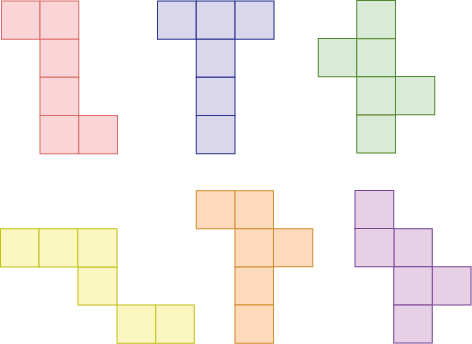
\includegraphics[width=3.00278in,height=1.75833in]{media/image36.png}João
possui uma distribuidora de ovos e acabou de receber 14 caixas com 310
ovos cada uma. Para que João venda essa mercadoria, ele faz embalagens
de 12 ovos. Quantas embalagens João conseguirá fazer para
colocar à venda os ovos que acabou de receber? Haverá alguma sobra?

https://img.freepik.com/fotos-gratis/ovos-na-superficie-rosa\_58702-1950.jpg?w=1060\&t=st=1677435684\textasciitilde{}exp=1677436284\textasciitilde{}hmac=6c6204dcded4c4d80a06169fee49d53df4b2636105a2c7b3dbe5365007ceae9a

Deixar retângulo em branco equivalente a 3 linhas para os cálculos.

Resposta:

(14 x 310) : 12 = 361 embalagens com 12 ovos cada uma e uma sobra de 8
ovos.

Professor sempre escreva a expressão formada pela interpretação do
enunciado, pois assim os alunos vão aprendendo a transformar textos em linguagem
matemática.

\subsubsection{8.}\label{section-20}

O livro que Gabriel está lendo possui 12 capítulos com 22 páginas cada
um. Se ele ler 10 páginas por dia, em quantos dias ele terminará de ler
o livro?

Deixar retângulo em branco equivalente a 3 linhas para a resolução

Resposta:

(12 x 22) : 10 = 26 dias lendo 10 páginas por dia e 1 dia lendo 4 páginas; portanto terminará o livro em 27 dias.

\subsubsection{9.}\label{section-21}

O pai de Pedro propôs a ele um grande desafio:
o pai fornece uma conta com um número escondido e o filho 
descobre qual número está escondido. Ajude Pedro com esse desafio e
encontre o número que está escondido pelo ponto de interrogação.

  4.670
--3.?50
________
  1.520

O algarismo escondido é o 1.

\subsubsection{10.}\label{section-22}

Na fazendo do avô de Vinícius, há 104 galinhas, 62 porcos, 6 cavalos e 72
bois. Se na fazendo de seu vizinho o número de animais é o triplo do que
há na fazenda do avô, quantos animais estão presentes na fazenda do
vizinho?

Deixar retângulo em branco equivalente a 3 linhas para a resolução

Resposta:

Número de animais na fazenda do avô: 104 + 62 + 6 + 72 = 244 animais.

Número de animais na fazenda do vizinho: 244 x 3 = 732 animais.

\subsection{Treino}\label{treino-1}

\subsubsection{1.}\label{section-23}

Verificando algumas atividades realizadas na escola no ano anterior,
Gustavo se deparou com uma conta em que 417 era o minuendo, mas o subtraendo
estava coberto por um retângulo. A diferença estava visível: 105.
Gustavo ficou curioso e resolveu refazer a atividade para descobrir o
número que faltava e, após alguns minutos, conseguiu descobrir. O número
que Gustavo encontrou é o

\begin{enumerate}
\def\labelenumi{\alph{enumi})}
\item
  128.
\item
  312.
\item
  158.
\item
  256.
\end{enumerate}

SAEB: Calcular o resultado de adições ou subtrações envolvendo números naturais de até 6 ordens.
BNCC: EF04MA07 -- Resolver e elaborar problemas de divisão cujo divisor tenha no máximo dois algarismos,
envolvendo os significados de repartição equitativa e de medida, utilizando estratégias diversas,
como cálculo por estimativa, cálculo mental e algoritmos.
a) Incorreta. Cometeu-se um erro na segunda etapa da conta.
b) Correta. 417 – 105 = 312.
c) Incorreta. Cometeu-se um erro na segunda etapa da conta.
d) Incorreta. Todo o procedimento foi errado.


\subsubsection{2.}\label{section-24}

Isaac estava conferindo o estoque de mercadorias de sua loja e percebeu
que inicialmente ele tinha 200 peças. Depois vendeu 2 caixas com peças
para Carlos. Em cada uma das caixas havia um pacote com 5 unidades de peças e dois
pacotes com 7 peças. Para saber a quantidade de peças que restavam no estoque, Isaac fez a
seguinte anotação:

200 -- 2 x (1 x 5 + 2 x 7)

O resultado dessa expressão era exatamente igual à quantidade de peças
que restavam em seu estoque após a venda para Carlos. Qual é a
quantidade de peças que Isaac possui agora em seu estoque?

\begin{enumerate}
\def\labelenumi{\alph{enumi})}
\item
  72.
\item
  94.
\item
  126.
\item
  162.
\end{enumerate}

SAEB: Calcular o resultado de multiplicações ou divisões envolvendo números naturais de até 6 ordens.
BNCC: EF04MA07 -- Resolver e elaborar problemas de divisão cujo divisor tenha no máximo dois algarismos,
envolvendo os significados de repartição equitativa e de medida, utilizando estratégias diversas,
como cálculo por estimativa, cálculo mental e algoritmos.

a) Incorreta. Não foram operacionalizadas primeiro as multiplicações.
b) Incorreta. Cometeu-se um erro na ordem das operações.
c) Incorreta. O subtraendo da conta final foi calculado errado.
d) Correta. 200 -- 2 x (1 x 5 + 2 x 7) = 200 -- 2 x (5 + 14) = 200 -- 2 x 19 = 200 -- 38 = 162 peças.

\subsubsection{3.}\label{section-25}

Um grande circo chegou à cidade em que Rafael mora, e logo uma fila
enorme se formou com pessoas querendo assistir ao espetáculo. Os
ingressos começaram a ser vendidos e as pessoas começaram a entrar no
recinto do circo. Em certo instante sabia-se que 540 pessoas já tinham
entrado e que a capacidade máxima por espetáculo nesse circo era de 1.200 pessoas. Ainda estão na fila 932 pessoas. Quantas pessoas não
conseguirão entrar para assistir a essa sessão do circo?

\begin{enumerate}
\def\labelenumi{\alph{enumi})}
\item
  268.
\item
  272.
\item
  294.
\item
  440.
\end{enumerate}

SAEB: Resolver problemas de adição ou de subtração, envolvendo números naturais de até 6 ordens, com os significados de juntar, acrescentar, separar, retirar, comparar ou completar.
BNCC: EF04MA07 -- Resolver e elaborar problemas de divisão cujo divisor tenha no máximo dois algarismos,
envolvendo os significados de repartição equitativa e de medida, utilizando estratégias diversas,
como cálculo por estimativa, cálculo mental e algoritmos.

a) Incorreta. A subtração foi realizada incorretamente.
b) Correta. 1.200 –- 540 = 660 vagas. 932 –- 660 = 272 pessoas não conseguirão assistir à sessão.
c) Incorreta. Só foi calculado o número de lugares vazios.
d) Incorreta. Errou-se na primeira subtração.


\section{3. Sequências}\label{muxf3dulo-3}

\colorsec{Habilidades do SAEB}

\begin{itemize}
\item Inferir ou descrever atributos ou propriedades comuns que os elementos
que constituem uma sequência recursiva de números naturais apresentam.
\item Inferir o padrão ou a regularidade de uma sequência de números
naturais ordenados, objetos ou figuras.
\item Inferir os elementos ausentes em uma sequência de números naturais
ordenados, objetos ou figuras.
\end{itemize}

\colorsec{Habilidade da BNCC}

\begin{itemize}
\item EF04MA11.
\end{itemize}

\subsection{Conteúdo}\label{conteuxfado-2}

Uma sequência ou sucessão é um conjunto ordenado no qual
existe sempre uma lógica de formação. Veja exemplos a seguir.

\begin{itemize}
\item
  A escalação de um time de futebol de salão em ordem alfabética: Alan; Bruno; Fernando; Igor; Tácio.
\item
  A sequência de números naturais pares: (0; 2; 4; 6; 8; 10; 12; ...).
\end{itemize}

Podemos classificar as sequências quanto ao número de elementos:

\begin{itemize}
\item
  \textbf{Finitas}: apresentam um número de termos bem definido.
\item
  \textbf{Infinitas}: apresentam infinitos números de termos, como
  a sequência dos números naturais.
\end{itemize}

Ainda podemos classificar as sequências numéricas desta forma:

\begin{itemize}
\item
  \textbf{Crescentes}: aquelas em que cada termo sucessor é maior que seu
  antecessor. Exemplo: (5, 10, 15, 20, 25).
\item
  \textbf{Decrescentes}: aquelas em que cada termo sucessor é menor que
  seu antecessor. Exemplo: (9, 7, 5, 3).
\end{itemize}

\subsection{Atividades}\label{atividades-2}

\subsubsection{1.}\label{section-26}

Observe as sequências dadas e determine o oitavo termo.

\begin{escolha}
  \item (4; 7; 10; 13...)
Resposta: (8 x 3) + 1 = 25
  \item (3; 6; 9...)
Resposta: 8 x 3 = 24
  \item (4; 8; 12...)
Resposta: 8 x 4 = 32
  \item (5; 10; 15; 20...)
Resposta: 8 x 5 = 40
\end{escolha}

\subsubsection{2.}\label{section-27}

Observe atentamente a sequência numérica que Robson construiu e depois
faça o que se pede.

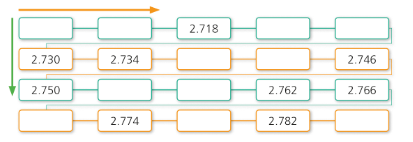
\includegraphics[width=3.44197in,height=1.18344in]{media/image43.png}

\begin{enumerate}
\def\labelenumi{\alph{enumi})}
\item
  Qual lógica Robson utilizou para construir essa sequência?
\end{enumerate}

Deixar espaço em branco equivalente a 3 linhas para a resolução

\begin{enumerate}
\def\labelenumi{\alph{enumi})}
\item
  Complete a sequência com os números que estão faltando.
\end{enumerate}

Resposta:

\begin{enumerate}
\def\labelenumi{\alph{enumi})}
\item
  Em cada coluna, ele foi aumentando os números em 10 unidades, enquanto,
  em cada linha, o aumento foi de 4 unidades. Outra forma de pensar é que, seguindo as setas colocadas
por ele, o aumento sempre foi de 4 unidades de um número para o próximo.

Professor explore as duas situações com os alunos.

\begin{enumerate}
\def\labelenumi{\alph{enumi})}
\item
  Linha 1: 2.710; 2.714; 2.718; 2.722; 2.726.
\end{enumerate}

Linha 2: 2.730; 2.734; 2.738; 2.742; 2.746.

Linha 3: 2.750; 2.754; 2.758; 2.762; 2.766.

Linha 4: 2.770; 2.774; 2.778. 2.782; 2.786.


\subsubsection{3.}\label{section-28}

Encontre o número pedido em cada item a seguir.

\begin{enumerate}
\def\labelenumi{\alph{enumi})}
\item
  O sucessor de 4.089.\_\_\_\_4 090\_\_\_\_\_\_\_\_\_
\item
  O antecessor de 5.301 \_\_\_5 300\_\_\_\_\_\_\_\_
\item
  O sucessor e o antecessor do número 4.259.\_\_4.258 e 4.260\_\_\_\_\_\_\_\_
\end{enumerate}


\subsubsection{4.}\label{section-29}

Entre os cadernos de seu irmão, Ana Clara encontrou um papel em que estava escrito assim: (231; 288; 245; 402; ...). Ela ficou muito curiosa, pois entendeu que essa era uma sequência
numérica, e queria encontrar o próximo número. Ajude Ana Clara a descobrir qual é o próximo número da sequência e o
escreva no espaço a seguir.

Deixar 1 linha para resposta

Resposta:

A sequência foi montada sempre somando-se 57 ao número anterior para
encontrar o próximo. Portanto o próximo número da sequência será: 402 +
57 = 459.

\subsubsection{5.}\label{section-30}

Organize os números a seguir em ordem decrescente.

11.010 --- 10.111 --- 11.100 --- 11.111 --- 11.000 --- 1.111 --- 10.001

Resposta:

Ordem decrescente (do maior para o menor):
11.111; 11.100; 11.010; 11.000; 10.111; 10.001; 1.111.

\subsubsection{6.}\label{section-31}

O Pai de André montou a sequência de figuras a seguir.

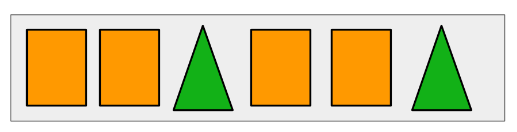
\includegraphics[width=4.30871in,height=1.10010in]{media/image45.png}

Em seguida, disse ao filho que o levaria ao cinema caso ele acertasse
qual seria o 20º termo dessa sequência. André, muito empolgado, começou a
pensar e logo deu a resposta a seu pai. O pai analisou a resposta e
disse que estava correta. Qual resposta André deu a seu pai sobre qual era o décimo elemento
dessa sequência?

Deixar 3 linhas para resposta e cálculos

Resposta:

Só teremos triângulos em múltiplos de 3. Como 20 não é um
múltiplo de 3, a vigésima figura será um quadrado.

\coment{É possível que o aluno continue a sequência com desenhos até
chegar à resposta. Não há problema nisso, e é muito válido, pois assim
entenderão a lógica envolvida.}

\subsubsection{7.}\label{section-32}

Relembre os conceitos de números naturais pares e ímpares e em seguida
responda ao que se pergunta a seguir.

\begin{enumerate}
\def\labelenumi{\alph{enumi})}
\item
  Escreva os 10 primeiros números naturais pares em sequência crescente.
  Essa sequência é finita ou infinita? Como ela é formada?
\end{enumerate}

Deixar espaço de 3 linhas para a resposta.

Resposta:

(0; 2; 4; 6; 8; 10; 12; 14; 16; 18). Essa é uma sequência finita e sempre
somamos 2 ao termo anterior para encontrar o próximo.

\begin{enumerate}
\def\labelenumi{\alph{enumi})}
\item
  Escreva os 12 primeiros números naturais ímpares em sequência
  crescente. Essa sequência é finita ou infinita? Como ela é formada?
\end{enumerate}

Deixar espaço de 3 linhas para a resposta.

Resposta:

(1; 3; 5; 7; 9; 11; 13; 15; 17; 19; 21; 23). Essa é uma sequência finita
e sempre somamos 2 ao termo anterior para encontrar o próximo.

\coment{Explore com os alunos o conceito de que, na sequência dos
números naturais, após um número par sempre aparece um numero ímpar, ou seja,
eles se intercalam.}

\subsubsection{8.}\label{section-33}

Estudando com a filha, Luísa, para a prova de Matemática da semana seguinte,
Laura propõe à menina o exercício a seguir.

Escreva uma sequência de 6 números que aumenta de 12 em 12 unidades,
começando pelo número nove mil e novecentos e noventa e nove.

Ajude Luísa a resolver esse exercício, escrevendo os seis números
pedidos.

Deixar espaço de 2 linhas para a resposta.

Resposta:

A sequência é: (9.999; 10.011; 10.023; 10.035; 10.047; 10.059).

\subsubsection{9.}\label{section-34}

Monte cada uma das sequências propostas a seguir, com seis números cada uma.

\begin{enumerate}
\def\labelenumi{\alph{enumi})}
\item
  Sequência de números que começa no 222 e aumenta de 9 em 9 unidades.
\end{enumerate}

Deixar espaço de 2 linhas para a resposta.

\begin{enumerate}
\def\labelenumi{\alph{enumi})}
\item
  Sequência de números que começa no 30 e aumenta de 50 em 50 unidades.
\end{enumerate}

Deixar espaço de 2 linhas para a resposta.

\begin{enumerate}
\def\labelenumi{\alph{enumi})}
\item
  Sequência de números que começa no 220 e diminui de 5 em 5 unidades.
\end{enumerate}

Deixar espaço de 2 linhas para a resposta.

Respostas:

\begin{enumerate}
\def\labelenumi{\alph{enumi})}
\item
  (222; 231; 240; 249; 258; 267).
\item
  (30; 80; 130; 180; 230; 280).
\item
  (220; 215; 210; 205; 200; 195).
\end{enumerate}

\subsubsection{10.}\label{section-35}

Observe as sequências a seguir e as complete com os números que estão
faltando.

\begin{enumerate}
\def\labelenumi{\alph{enumi})}
\item
\end{enumerate}

\begin{longtable}[]{@{}llllll@{}}
\toprule
5 862 & 6 862 & 7 862 &  &  & 10 862\tabularnewline
\bottomrule
\end{longtable}

\begin{enumerate}
\def\labelenumi{\alph{enumi})}
\item
\end{enumerate}

\begin{longtable}[]{@{}llllll@{}}
\toprule
198 & 190 &  & 174 &  & \tabularnewline
\bottomrule
\end{longtable}

Respostas:

\begin{enumerate}
\def\labelenumi{\alph{enumi})}
\item
  (5.862; 6.862; 7.862; 8.862; 9.862; 10,862).
\item
  (198; 190; 182; 174; 166; 158).
\end{enumerate}

\subsection{Treino}\label{treino-2}

\subsubsection{1.}\label{section-36}

Observe a sequência a seguir.

\begin{itemize}
  \item Figura 1: duas bolinhas.
  \item Figura 2: seis bolinhas.
  \item Figura 3: doze bolinhas.
  \item Figura 4: vinte bolinhas.
\end{itemize}

 A figura 6 terá

\begin{enumerate}
\def\labelenumi{\alph{enumi})}
\item
  25 bolinhas.
\item
  30 bolinhas.
\item
  35 bolinhas.
\item
  42 bolinhas.
\end{enumerate}

SAEB: Inferir o padrão ou a regularidade de uma sequência de números naturais ordenados, objetos ou figuras.
BNCC: EF04MA11 -- Identificar regularidades em sequências numéricas compostas por múltiplos de um
número natural.
a) Incorreta. O aluno não entendeu a lógica da sequência.
b) Incorreta. O aluno não identificou o padrão.
c) Incorreta. O aluno chegou a um número menor que o da resposta correta.
d) Correta. A sequência é esta: (2; 6; 12; 20; 30; 42).


\subsubsection{2.}\label{section-37}

Ana Amélia encontrou a seguinte sequência numérica e ficou curiosa, pois
faltava um número para ser escrito.

45.205 --- 45.305 --- 45.405 --- 45.505 --- ? --- 45.705

Utilizando seus conhecimentos matemáticos, Ana Amélia chegou à conclusão de que
faltava o número

\begin{enumerate}
\def\labelenumi{\alph{enumi})}
\item
  45.505.
\item
  45.605.
\item
  45.705.
\item
  45.205.
\end{enumerate}

SAEB: Inferir os elementos ausentes em uma sequência de números naturais ordenados, objetos ou figuras.
BNCC: EF04MA11 -- Identificar regularidades em sequências numéricas compostas por múltiplos de um
número natural.
a) Incorreta. O aluno se confundiu com o antecessor do número que falta.
b) Correta. A sequência aumenta de 100 em 100 unidades.
c) Incorreta. O aluno se confundiu com o sucessor do número que falta.
d) Incorreta. O aluno selecionou, incorretamente, o primeiro número da sequência.


\subsubsection{3.}\label{section-38}

Dois aplicativos exigem uma senha numérica para serem acessados. Breno
criou a senha 7081 para o primeiro e para o segundo utilizou como senha
o sucessor do sucessor do número escolhido para a primeira senha. A
senha utilizada por Breno para o segundo aplicativo é

\begin{enumerate}
\def\labelenumi{\alph{enumi})}
\item
  7079.
\item
  7080.
\item
  7082.
\item
  7083.
\end{enumerate}

SAEB: Inferir ou descrever atributos ou propriedades comuns que os elementos que constituem uma sequência recursiva de números naturais apresentam.
BNCC: EF04MA11 -- Identificar regularidades em sequências numéricas compostas por múltiplos de um
número natural.
a) Incorreta. Esse é o antecessor do antecessor.
b) Incorreta. Esse é o antecessor.
c) Incorreta. Esse é o sucessor.
d) Correta. O sucessor do sucessor de 7081 é 7081 + 1 + 1 = 7083.


\section{4. Grandezas e medidas}\label{muxf3dulo-4}

\colorsec{Habilidades do SAEB}

\begin{itemize}
\item Reconhecer a unidade de medida ou o instrumento mais apropriado para
medições de comprimento, área, massa, tempo, capacidade ou temperatura.
\item Estimar/inferir medida de comprimento, capacidade ou massa de objetos,
utilizando unidades de medida convencionais ou não ou medir comprimento,
capacidade ou massa de objetos.
\item Explicar que o resultado de uma medida depende da unidade de medida
utilizada.
\item Resolver problemas que envolvam medidas de grandezas (comprimento,
massa, tempo e capacidade) em que haja conversões entre as unidades mais
usuais.
\item Determinar o horário de início, o horário de término ou a duração de
um acontecimento.

\colorsec{Habilidades da BNCC}

\begin{itemize}
\item EF04MA20, EF04MA23.
\end{itemize}

\subsection{Conteúdo}\label{conteuxfado-3}

\begin{itemize}
  \item Medidas de comprimento:
  quilômetro (km), hectômetro (hm), decâmetro (dam), \textbf{metro (m)}, decímetro (dm), centímetro (cm), milímetro (mm).
  \item Medidas de massa:
  quilograma (kg), hectograma (hg), decagrama (dag), \textbf{grama(g)}, decigrama (dg), centigrama (cg), miligrama (mg).
  \item Medidas de capacidade:
  quilolitro (kL), hectolitro (hL), decalitro (daL), \textbf{litro(L)}, decilitro (dL), centilitro (cL), mililitro (mL).
  \item Medidas de tempo:
  1 dia = 24 horas (h) = 1.440 minutos (min) = 86.400 segundos (s).

\subsection{Atividades}\label{atividades-3}

\subsubsection{1.}\label{section-39}

Relacione as quantidades que estão na coluna da esquerda com a leitura correta
correspondente na leitura da direita.

1,935 kg Trinta e cinco centímetros

2,340 km Um quilo e novecentos e trinta e cinco gramas

0,400 g Dois quilômetros e trezentos e quarenta metros

0,35 m Quatrocentos miligramas

Respostas:

1,935 kg = um quilo e novecentos e trinta e cinco gramas.
2,340 km = Dois quilômetros e trezentos e quarenta metros.
0,400 g = quatrocentos miligramas.
0,35 m = trinta e cinco centímetros.

\subsubsection{2.}\label{section-40}

Para cada item a seguir, forneça o número de décadas correspondente.

\begin{escolha}
\item Hipopótamo: vive em média 40 anos.
Resposta: 4 décadas.
\item Camelo: vive em média 50 anos.
Resposta: 5 décadas.
\item Leão: vive em média 20 anos.
Resposta: 2 décadas.
\item Elefante: vive em média 70 anos.
Resposta: 7 décadas.
\item Tartaruga: vive em média 100 anos.
Resposta: 10 décadas.
\item Arara: vive em média 60 anos.
Resposta: 6 décadas.


\subsubsection{3.}\label{section-41}

Pinte a bolinha que corresponde à capacidade total de líquido que há em cada caso.

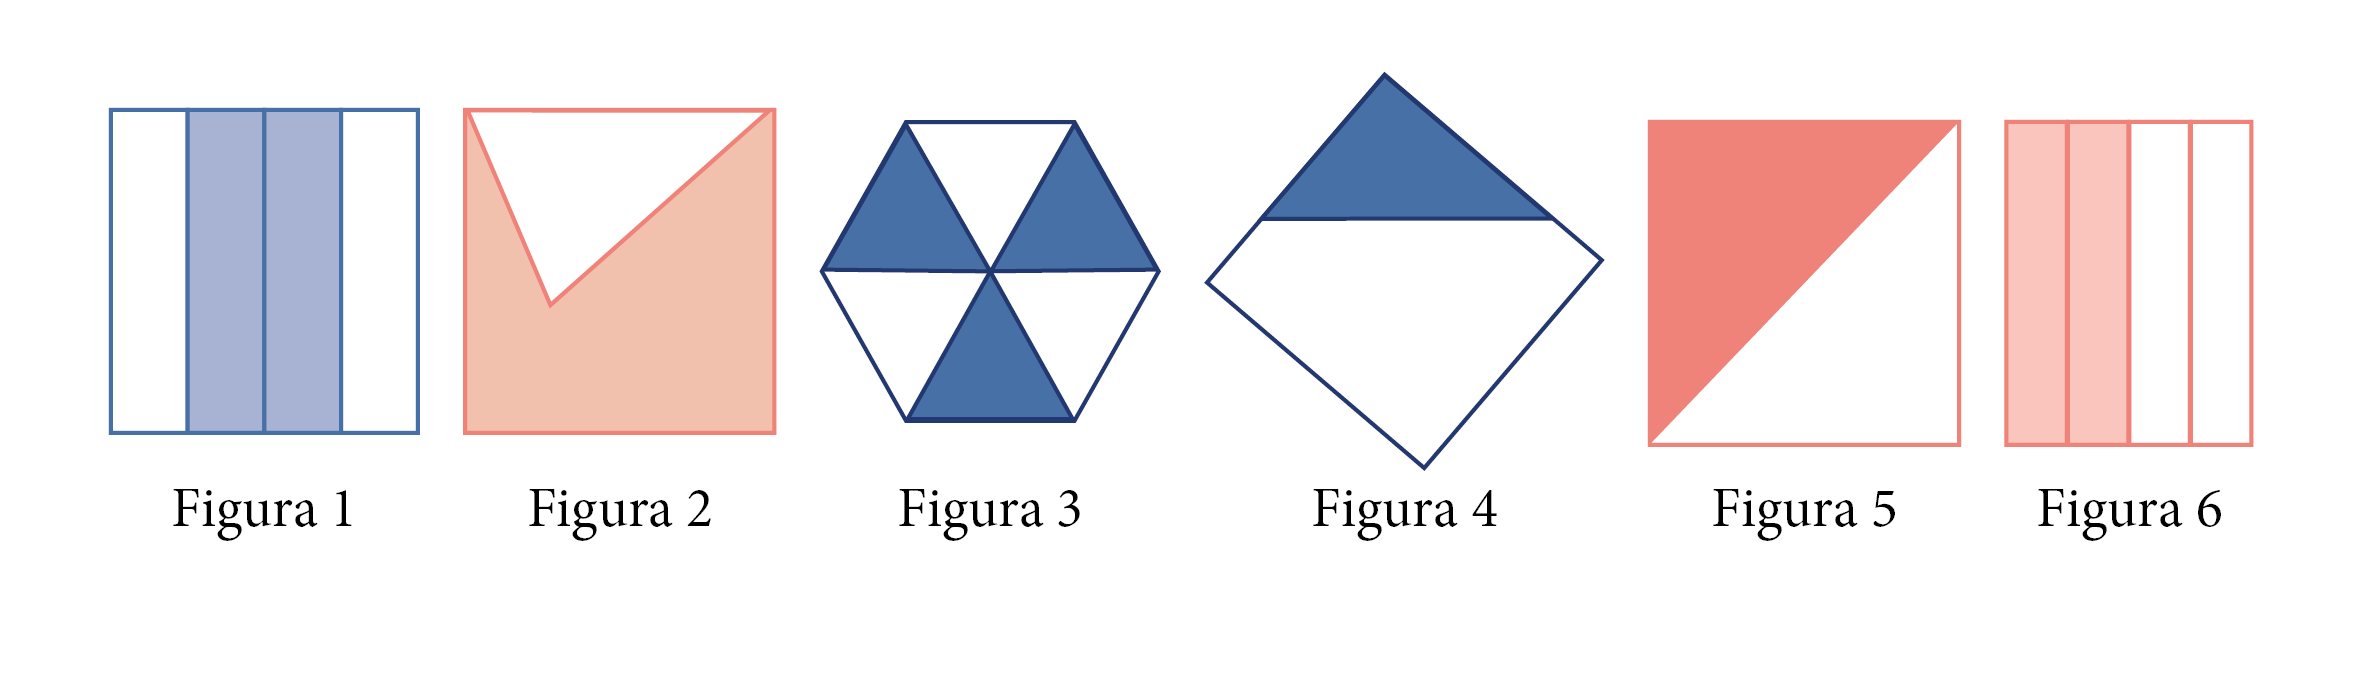
\includegraphics[width=4.17536in,height=3.42530in]{media/image52.png}

Resposta:

Duas unidades de limpador multiuso de 500 mL totalizam 1 litro.
Três unidades de loção hidratante de 150 mL totalizam 450 mL (menos que 0,5 L).
Quatro unidades de bebida energética de 330 mL totalizam 1.320 mL (menos que 1,5 L).
Quatro unidades de amaciante de roupa de 1.000 mL totalizam 4.000 ml = 4 L (mais
que 3,5 L).

\subsubsection{4.}\label{section-42}

A empresa em que Rafael trabalha vende suco de frutas com embalagens de
diversas capacidades: 200 mL, 250 mL, 333 mL e 1,5 L. Com base nisso, responda ao que se pergunta a seguir.

\begin{enumerate}
\def\labelenumi{\alph{enumi})}
\item
  Uma pessoa quer adquirir o volume de suco da maior embalagem,
  mas quer comprar a embalagem de 250 mL. Quantas embalagens deverão ser adquiridas?
\end{enumerate}

Deixar espaço em branco equivalente a 3 linhas para a resolução
A embalagem maior possui 1.500 mL, o que corresponde a 6 embalagens de 250 mL.

\begin{enumerate}
\def\labelenumi{\alph{enumi})}
\item
  Oito embalagens de 250 mL equivalem a quantas embalagens de 200 mL?
\end{enumerate}

Deixar espaço em branco equivalente a 3 linhas para a resolução
8 x 250 = 2.000 mL, o que equivale a 10 embalagens de 200 mL.


\subsubsection{5.}\label{section-43}

Um dos brinquedos do parque de diversões permanente de uma cidade proíbe
que crianças com uma altura menor que 1,20 m possam brincar em determinada
atração. Manoel mediu sua altura e ele está com 93 cm. Quanto ele
precisa crescer para poder realizar seu sonho de brincar nessa atração?

Deixar espaço em branco equivalente a 2 linhas para cálculos

Resposta:

1,20 m = 120 cm

120 -- 93 = 23 cm

Ele ainda precisará crescer 23 cm para que esteja apto a brincar na atração.

\subsubsection{6.}\label{section-44}

Roberta utiliza um termômetro profissional para medir a temperatura da
água que vai utilizar para fazer uma deliciosa receita de rosca
caseira. A receita diz que a temperatura da água deve ser exatamente 74ºC
para que possa ser adicionada. Em determinado momento, Roberta colocou
o termômetro na água e observou a seguinte temperatura: 63ºC. Podemos concluir que

\begin{enumerate}
\def\labelenumi{\alph{enumi})}
\item
  Roberta já pode adicionar a água à receita.
\item
  a água está mais quente do que o necessário; sendo assim, será
  necessário esfriar um pouco para que possa ser adicionada.
\item
  a água está 11ºC abaixo da temperatura ideal; sendo assim, ainda
  precisa aquecer um pouco.
\item
  Roberta não tem dados para analisar se adiciona ou não a água à receita.
\end{enumerate}

Como a temperatura indicada no termômetro é de 63ºC e a temperatura
ideal para a receita é de 74ºC, a água ainda deverá ser aquecida em 11ºC.

\subsubsection{7.}\label{section-45}

Observe as situações descritas a seguir e escreva o valor da massa (em quilogramas e em gramas) de cada item.

\begin{enumerate}
\def\labelenumi{\alph{enumi})}
\item
  Para equilibrar os pratos de uma balança para pesar um saco de tomates, foram colocados um peso de 1 kg, outro de 500 g e outro de 100 g.
\item
  Para equilibrar os pratos de uma balança para pesar um saco de batatas, foram colcoados um peso de 1 kg e outro de 500 g.
\item
  Para equilibrar os pratos de uma balança para pesar um saco de cenouras, foram colocados dois pesoas de 1 kg, um de 500 g, outro de 100 g e outro de 50 g.
\item
  Para equilibrar os pratos de uma balança para pesar um saco de cebolas, foram colocados um peso de 1 kg, dois pesos de 500 g, outro de 50 g e três outros de 10 g.
\end{enumerate}

Respostas:

\begin{enumerate}
\def\labelenumi{\alph{enumi})}
\item
  1,6 kg = 1.600 g.
\item
  1,5 kg = 1.500 g.
\item
  2,65 kg = 2.650 g.
\item
  2,06 kg = 2.060 g.
\end{enumerate}

\subsubsection{8.}\label{section-46}

Para a festa de aniversário de Arthur, seu pai encomendou 24 garrafas de
refrigerante. Dessas garrafas, 10 continham 3 litros (cada uma). Nas
demais garrafas, havia dois litros em cada uma. Com base nessas
informações responda ao que se pergunta a seguir.

\begin{enumerate}
\def\labelenumi{\alph{enumi})}
\item
  Qual é a quantidade de refrigerante, em mililitros, encomendada pelo pai de Arthur?
\end{enumerate}

Deixar espaço em branco equivalente a 3 linhas para cálculos

\begin{enumerate}
\def\labelenumi{\alph{enumi})}
\item
  Se cada convidado da festa consumiu exatamente 400 mililitros de refrigerante e
  todo o refrigerante foi consumido durante a festa, quantas pessoas
  foram ao aniversário de Arthur?
\end{enumerate}

Deixar espaço em branco equivalente a 2 linhas para cálculos

Resposta:

\begin{enumerate}
\def\labelenumi{\alph{enumi})}
\item
  (10 x 3) + (14 x 2) = 30 + 28 = 58 L = 58 000 mL.
\item
  58.000 : 400 = 145 pessoas compareceram à festa.
\end{enumerate}

\subsubsection{9.}\label{section-47}

O comprimento de uma escrivaninha é de 1,6 m. Quantos palmos,
aproximadamente, mede a escrivaninha se, em média, um palmo tem 23 cm?

\begin{enumerate}
\def\labelenumi{\alph{enumi})}
\item
  5 palmos.
\item
  6 palmos.
\item
  7 palmos.
\item
  8 palmos.
\end{enumerate}

1,6 m = 160 cm

160 : 23 = 6,95 palmos (aproximadamente 7 palmos).

\subsubsection{10.}\label{section-48}

Ana Luísa deve tomar um remédio de 8 em 8 horas. Se ela tomou o primeiro
comprimido às 6 horas da manhã, qual será o horário em que ela deverá tomar
o terceiro comprimido?

Deixar espaço em branco equivalente a 3 linhas para a resolução

Resposta:

Primeiro comprimido: 6 horas da manhã.
Segundo comprimido: 6 + 8 = 2 horas da tarde ou 14 horas.
Terceiro comprimido: 14 + 8 = 22 horas ou 10 horas da noite.

\subsection{Treino}\label{treino-3}

\subsubsection{1.}\label{section-49}

Reinaldo foi contratado por uma empresa que possui um horário bem rígido.
Veja a seguir.

\begin{longtable}[]{@{}lll@{}}
\toprule
& Entrada & Saída\tabularnewline
\midrule
\endhead
Manhã & 8:00 & ?\tabularnewline
Tarde & 14:00 & 17:30\tabularnewline
\bottomrule
\end{longtable}


No período da manhã, Reinaldo deve
cumprir 4 horas e 30 minutos de trabalho. Qual será o horário em que
Reinaldo sairá para almoçar?

\begin{enumerate}
\def\labelenumi{\alph{enumi})}
\item
  11:00.
\item
  11:30.
\item
  12:00.
\item
  12:30.
\end{enumerate}

SAEB: Determinar o horário de início, o horário de término ou a duração de um acontecimento.
BNCC: EF04MA22 -- Ler e registrar medidas e intervalos de tempo em horas, minutos e segundos em
situações relacionadas ao seu cotidiano, como informar os horários de início e término de realização
de uma tarefa e sua duração.
a) Incorreta. O aluno somou uma hora e meia a menos.
b) Incorreta. O aluno somou uma hora a menos.
c) Incorreta. O aluno somou meia hora a menos.
d) Correta. 8 + 4,5 = 12,5 (12:30).


\subsubsection{2.}\label{section-50}

Na receita médica de Marcela, recomenda-se que ela tome um xarope 4 vezes ao
dia e que, em cada vez, ela tome a quantidade de 8 mL durante 15 dias. Um
frasco do remédio contém 100 mL. Qual é a quantidade de
frascos que a mãe de Marcela deverpa comprar para que todo o tratamento
seja concluído?

\begin{enumerate}
\def\labelenumi{\alph{enumi})}
\item
  2.
\item
  3.
\item
  4.
\item
  5.
\end{enumerate}

SAEB: Estimar/inferir medida de comprimento, capacidade ou massa de objetos, utilizando unidades de medida convencionais ou não ou medir comprimento, capacidade ou massa de objetos.
BNCC: EF04MA20 -- Medir e estimar comprimentos (incluindo perímetros), massas e capacidades, utilizando
unidades de medida padronizadas mais usuais, valorizando e respeitando a cultura local.

a) Incorreta. O aluno chegou a um número menor que a metade do valor da resposta.
b) Incorreta. O aluno chegou a um valor que é maior que a metade do valor da resposta, mas ainda menor que a resposta.
c) Incorreta. O aluno se esqueceu de contar os 80 mL que ainda ficariam de fora da conta.
d) Correta. 4 x 8 x 15 = 480 mL. Como cada frasco possui 100 mL, ela deverá
comprar 5 frascos, e haverá uma sobra de xarope.

\subsubsection{3.}\label{section-51}

Vicente teve de fazer uma viagem para fechar um grande negócio. Se o voo
saiu do aeroporto às 10 horas e 42 minutos e chegou ao destino às 14
horas e 8 minutos, qual foi o tempo de duração do voo?

\begin{enumerate}
\def\labelenumi{\alph{enumi})}
\item
  11.760 segundos.
\item
  9.542 segundos.
\item
  5.364 segundos.
\item
  2.500 segundos.
\end{enumerate}

SAEB: Resolver problemas que envolvam medidas de grandezas (comprimento, massa, tempo e capacidade) em que haja conversões entre as unidades mais usuais.
BNCC: EF04MA22 -- Ler e registrar medidas e intervalos de tempo em horas, minutos e segundos em
situações relacionadas ao seu cotidiano, como informar os horários de início e término de realização
de uma tarefa e sua duração.

a) Correta. Se a partida do voo foi às 10 horas e 42 minutos e a chegada ao destino foi às 14 horas e 8 minutos, o tempo de voo foi de 3 horas e 16 minutos, ou seja, 196 minutos, o que equivale a 11.760 segundos.
b)Incorreta. O aluno errou na subtração entre os dois horários.
c)Incorreta. O aluno errou na conversão para segundos.
d) Incorreta. O aluno errou na subtração entre os dois horários e na conversão para segundos.


\section{5. Unidades e medidas}\label{muxf3dulo-5}

\colorsec{Habilidades do SAEB}

\begin{itemize}
\item Medir ou comparar perímetro ou área de figuras planas desenhadas em
malha quadriculada.
\item Identificar horas em relógios analógicos ou associar horas em relógios
analógicos e digitais.
\item Resolver problemas que envolvam perímetro de figuras planas.
\item Resolver problemas que envolvam área de figuras planas.
\end{itemize}

\colorsec{Habilidades da BNCC}

\begin{itemize}
\item EF04MA21, EF04MA22.
\end{itemize}

\subsection{Conteúdo}\label{conteuxfado-4}
Ampliação é o processo que realizamos quando queremos aumentar algo,
como, por exemplo, figuras planas, sem que suas características
sejam alteradas.

A figura menor a seguir teve o tamanho de todos os seus lados dobrado. Observe que manteve as mesmas
características.

Fazer a figura a seguir sem marcar os ângulos e a primeira deve ter lado
3 cm e a segunda lado 6 cm.

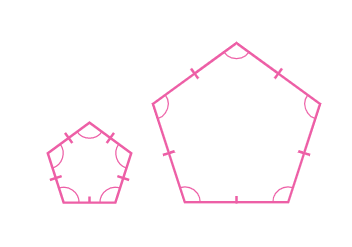
\includegraphics[width=2.21154in,height=1.55185in]{media/image56.png}

Redução é o processo que realizamos quando queremos diminuir algo,
como, por exemplo, figuras planas, sem que suas características
sejam alteradas.

A figura maior a seguir teve o tamanho de todos os seus lados dividido por dois. Observe que manteve as
mesmas características.

Fazer a figura a seguir sem marcar os ângulos e a primeira deve ter lado
6 cm e a segunda lado 3 cm.

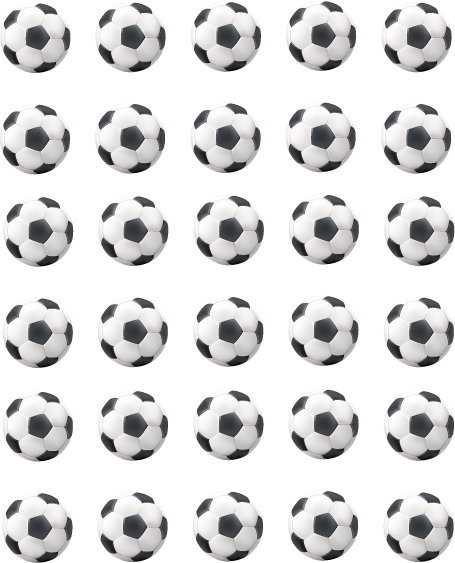
\includegraphics[width=2.44231in,height=1.44820in]{media/image57.png}

Muitas vezes, recorremos a malhas quadriculadas para nos
ajudar nesses processos. Com isso, é possível comparar áreas de
superfícies e até ter certeza de alguma ampliação ou alguma redução.

Outro instrumento muito útil é o relógio de ponteiros, que é dividido em doze partes ou
seções, numeradas de 1 a 12. Esses números representam as horas, marcadas pelo ponteiro menor.

Por sua vez, o intervalo de tempo que fica entre cada um dos números
representa a contagem dos minutos. Ficou convencionado que o
intervalo entre cada um deles é de 5 minutos. Então é necessário adicionar cinco minutos a cada número. Os minutos são marcados pelo ponteiro menor.

\subsection{Atividades}\label{atividades-4}

\subsubsection{1.}\label{section-52}

Aos finais de semana, Renato anda de bicicleta ao redor da praça
existente no bairro em que mora.

Construir uma figura como essa nos padrões do projeto.

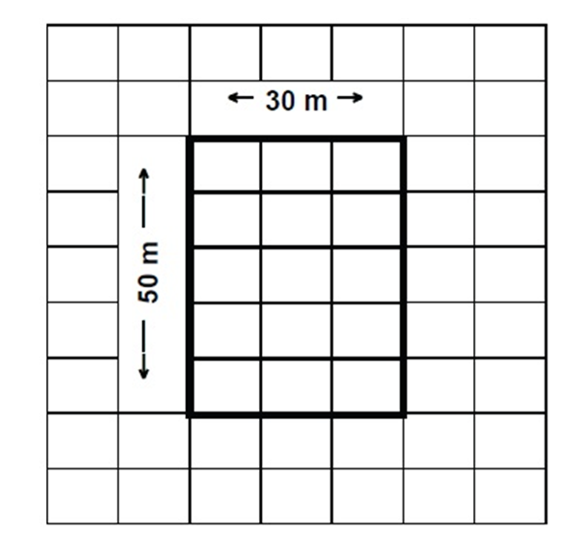
\includegraphics[width=2.35256in,height=2.20730in]{media/image61.png}

Se ele der seis voltas completas ao redor da praça, ele percorrerá qual
distância em quilômetros?

Deixar espaço em branco equivalente a duas linhas para cálculos

Resposta:

[(2 x 30) + (2 x 50)] x 6 = 960 m = 0,96 km.

\coment{Sempre que possível, estimule a montagem da expressão para que
os alunos comecem a se acostumar.}

\subsubsection{2.}\label{section-53}

Escreva por extenso as horas representadas a seguir. Depois, escreva uma atividade que você faz em cada um destes horários.

\begin{escolha}
  \item 12:30
  Doze horas e trinta minutos (ou meio-dia e meia).
  \item 14:15
  Quatorze horas e quinte minutos (ou duas e quinze da tarde).
  \item 6:30
  Seis horas e trinta minutos (ou seis e meia da manhã).
  \item 13:45
  Treze horas e quarenta e cinco minutos (ou quinze para as duas da tarde).
  \item 23:20
  Vinte e três horas e vinte minutos (ou onze e vinte da noite).
  \item 15:40
  Quinze horas e quarenta minutos (ou vinte para as quatro da tarde).
\end{escolha}

\subsubsection{3.}\label{section-54}

Leandro resolveu cobrir de azulejos o fundo de sua piscina de tal forma
que apareça, no fundo, a letra inicial do nome de seu filho Arnaldo.
Sabendo-se que cada quadradinho corresponde a um azulejo de 3 metros
quadrados de área, qual é a área que os azulejos utilizados
ocuparão?

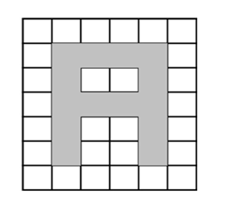
\includegraphics[width=1.42949in,height=1.25160in]{media/image63.png}

Construir uma figura conforme a anterior de acordo com os padrões do
projeto.

Deixar espaço em branco equivalente a 2 linhas para a resolução

Resposta:

14 quadradinhos x 3 = 42 metros quadrados.

\subsubsection{4.}\label{section-55}

Escreva no espaço correspondente quantos meses compõem um período de:

\begin{enumerate}
\def\labelenumi{\alph{enumi})}
\item
  2 anos:­­­­­­­­­­­­­­­­­­­\_\_\_24 meses\_\_\_\_\_\_\_\_\_\_
\item
  8 anos:\_\_\_96 meses\_\_\_\_\_\_\_\_\_\_
\item
  1 década:\_\_\_120 meses\_\_\_\_\_\_\_\_\_
\item
  1 século:\_\_\_1.200 meses\_\_\_\_\_\_\_\_
\end{enumerate}

\subsubsection{5.}\label{section-56}

Os desenhos representados a seguir representam as plantas baixas, inicial
e final, e o formato de uma praça que será construída em uma área
central de uma cidade. Inicialmente, a previsão era para uma praça
pequena, mas, como a prefeitura conseguiu uma área maior ao lado da
primeira, resolveu-se realizar a construção de uma praça maior.

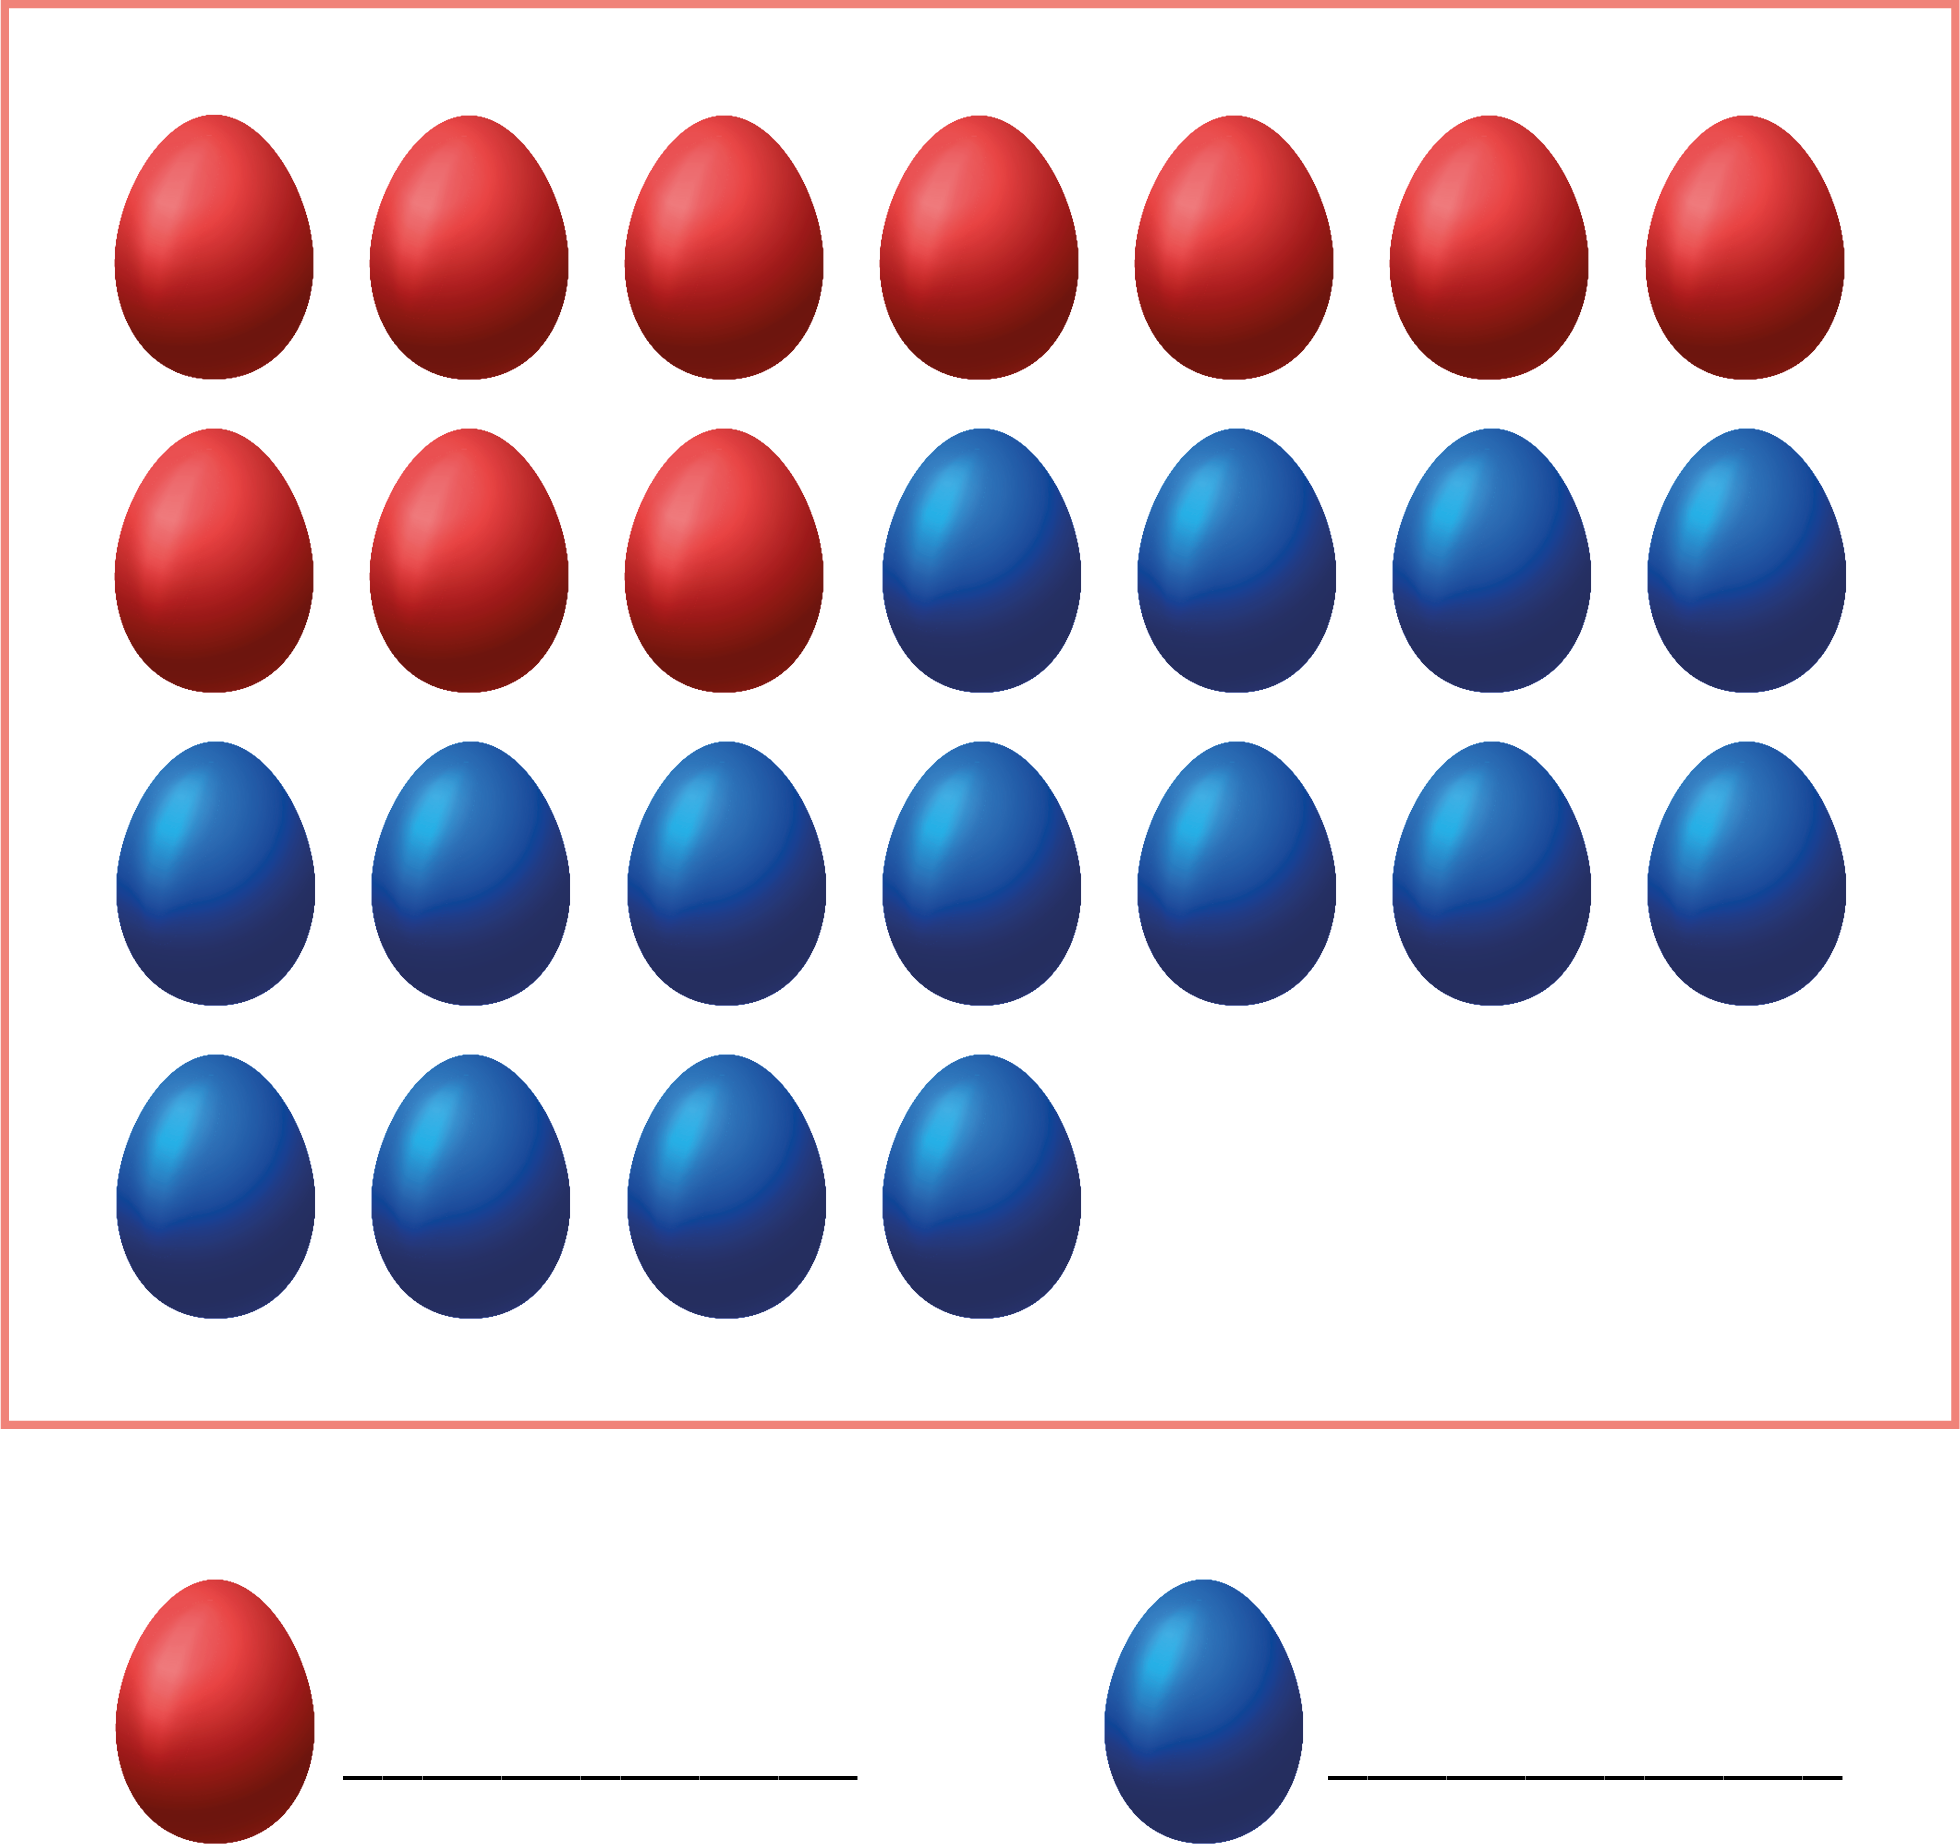
\includegraphics[width=5.00877in,height=1.80849in]{media/image64.png}

Construir uma figura conforme a anterior de acordo com os padrões do
projeto.

Sendo assim, com relação à praça que se desejava construir iniciamente,
a nova praça terá uma área

\begin{enumerate}
\def\labelenumi{\alph{enumi})}
\item
  2 vezes maior.
\item
  3 vezes maior.
\item
  4 vezes maior.
\item
  5 vezes maior.
\end{enumerate}

A praça menor teria 6 quadradinhos preenchendo sua área, enquanto a
grande terá 24 quadradinhos. Sendo assim, a área da praça maior é
quatro vezes a área da praça menor.

\subsubsection{6.}\label{section-57}

Observando-se atentamente as figuras, em que todos os quadradinhos têm a mesma área, pode-se perceber que a figura que
possui a menor área é a

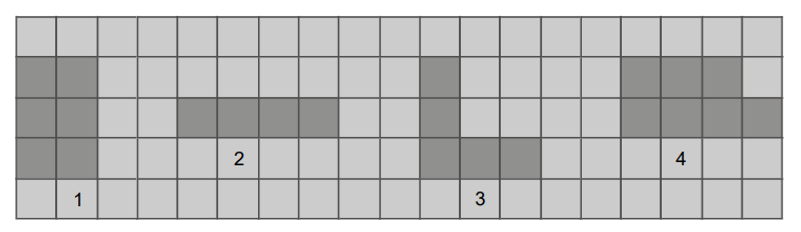
\includegraphics[width=5.12179in,height=1.48342in]{media/image65.png}

Construir uma figura conforme a anterior de acordo com os padrões do
projeto.

\begin{enumerate}
\def\labelenumi{\alph{enumi})}
\item
  1.
\item
  2.
\item
  3.
\item
  4.
\end{enumerate}

Resposta:

A figura 1 é composta de 6 quadradinhos. A figura 2 é composta de 4 quadradinhos.
A figura 3 é composta de 5 quadradinhos. A figura 4 é composta de 7 quadradinhos.
Como os quadradinhos são de mesmo tamanho, pode-se concluir que a figura
que possui a menor área é a figura 2, por ser composta de um número
menor de quadradinhos.

\subsubsection{7.}\label{section-58}

Um arquiteto fez um primeiro esboço de uma construção no formato de cruz
que teria de executar.

\begin{quote}

\includegraphics[width=2.27520in,height=1.51680in]{media/image66.png}
\end{quote}

Construir uma figura conforme a anterior de acordo com os padrões do
projeto.

\begin{quote}
No projeto final, todos os lados foram reduzidos à metade. Desenhe
a nova imagem do projeto.

\Paulo Deixar um retângulo em branco para os alunos desenharem.

\subsubsection{8.}\label{section-59}

Na malha quadriculada a seguir, cada quadrado representa uma área de 20
metros quadrados.

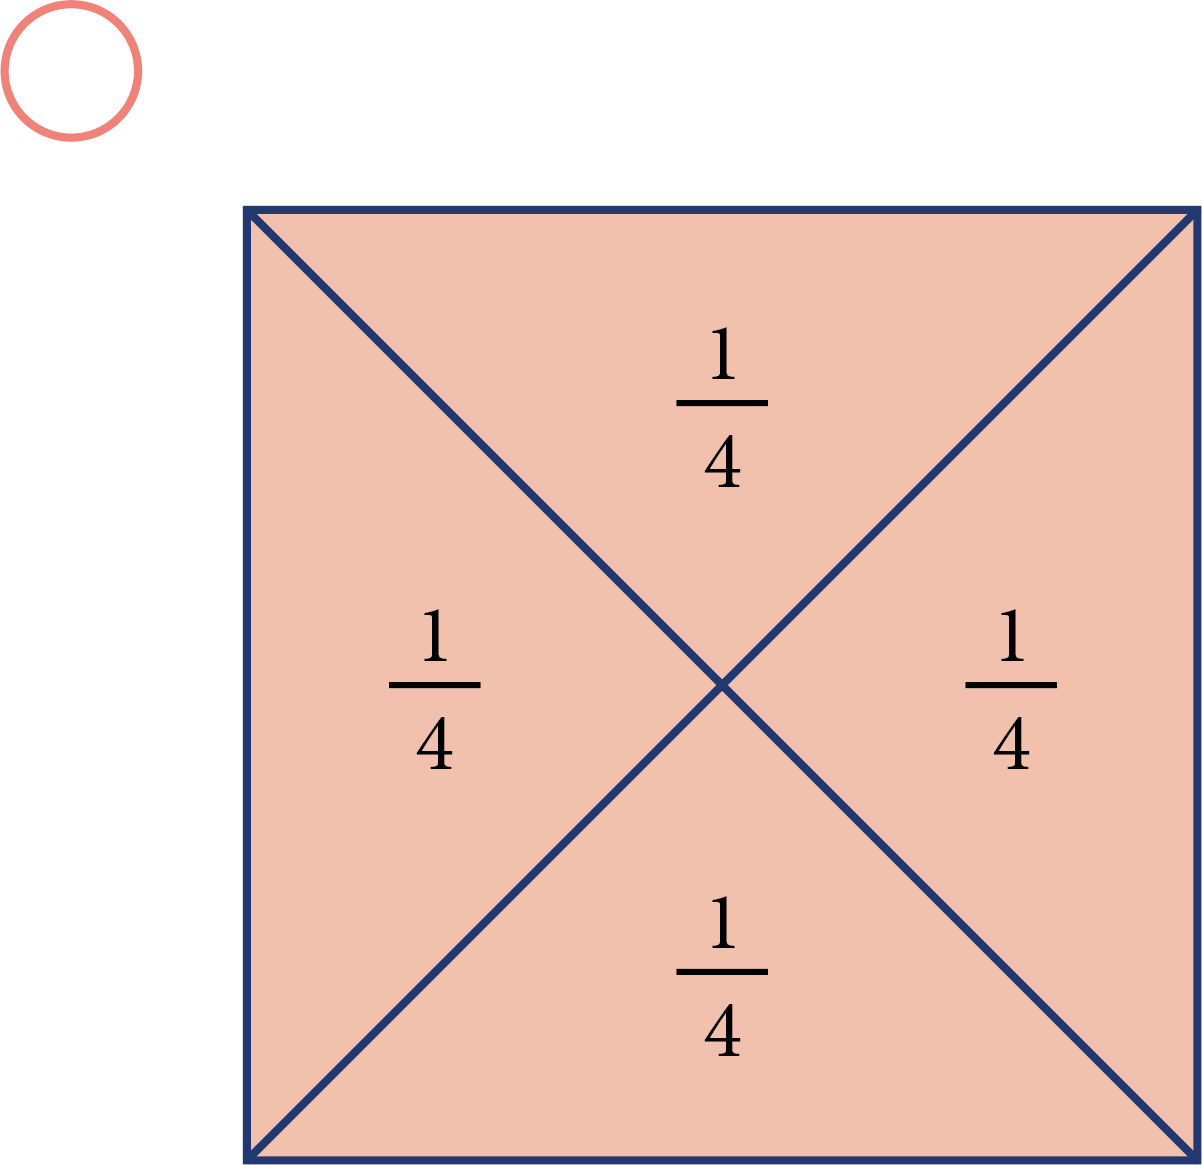
\includegraphics[width=3.33333in,height=1.50517in]{media/image68.png}

Construir uma figura conforme a anterior de acordo com os padrões do
projeto.

Qual é a área da malha quadriculada que a figura destacada ocupa?

Resposta:

Realizando-se a contagem de quadradinhos que preenchem a figura, chega-se
ao número 16. Portanto: 16 x 20 = 320 metros quadrados.

\subsubsection{9.}\label{section-60}

Entre alguns objetos de seu irmão mais velho, Gabriel encontrou a seguinte
malha quadriculada com letras destacadas.

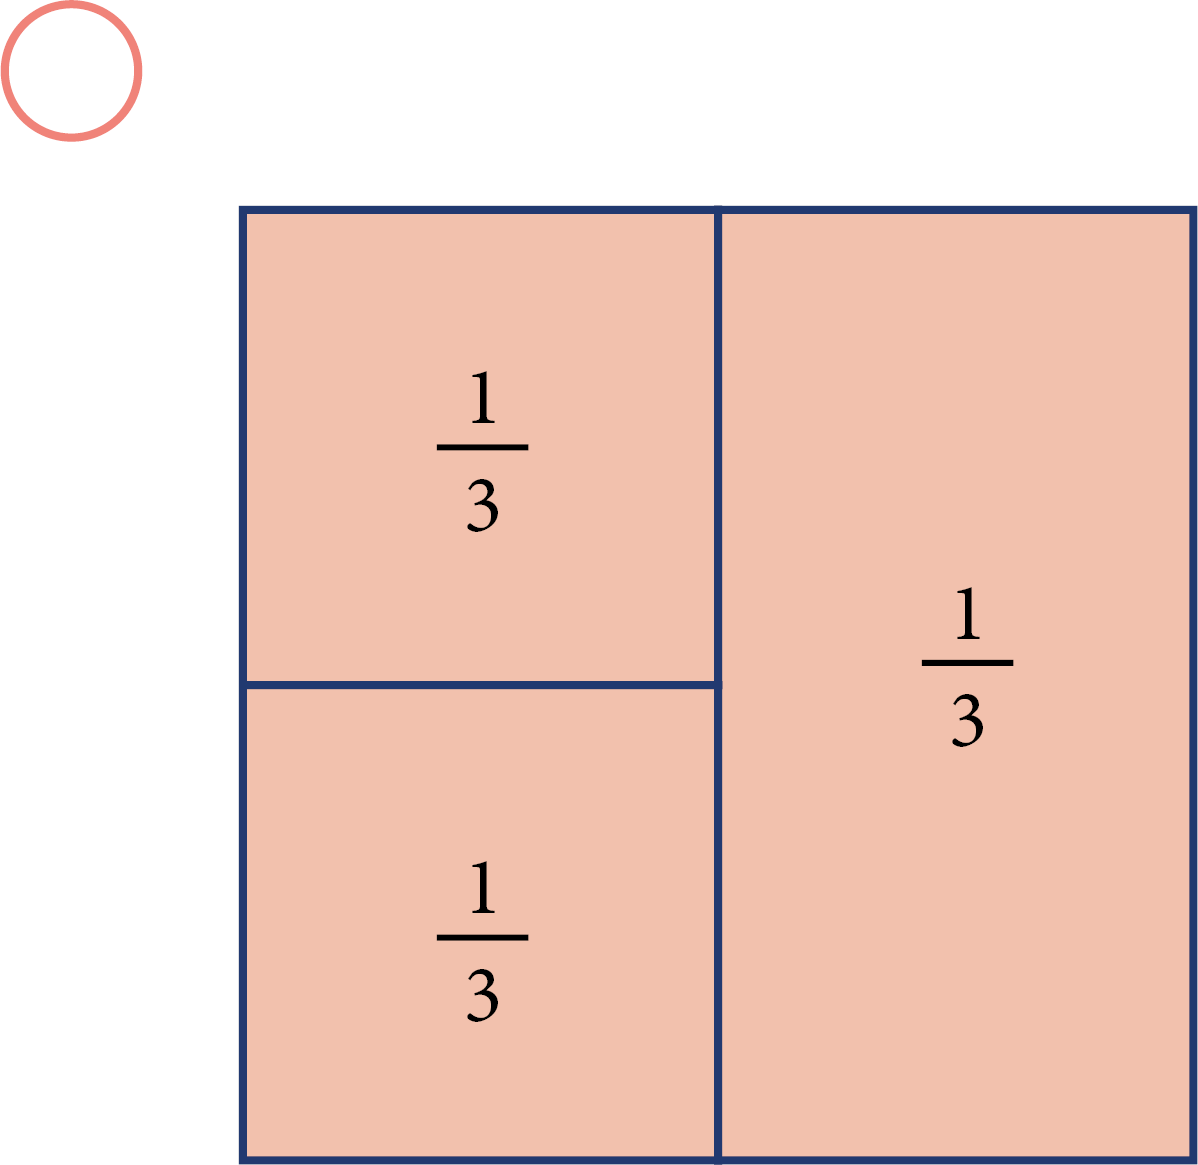
\includegraphics[width=4.36538in,height=1.60417in]{media/image69.png}

Construir uma figura conforme a anterior de acordo com os padrões do
projeto.

Entre essas letras, existem duas que ocupam superfícies de mesmo tamanho. Elas
são a

\begin{enumerate}
\def\labelenumi{\alph{enumi})}
\item
  A e a C.
\item
  D e a E.
\item
  D e a C.
\item
  A e a E.
\end{enumerate}

Letra A: 14 quadradinhos.
Letra C: 11 quadradinhos.
Letra D: 13 quadradinhos.
Letra E: 14 quadradinhos.
As duas letras que ocupam asuperfícies de mesmo tamanho são a A e a E.

\subsubsection{10.}\label{section-61}

Inês tem um compromisso inadiável às 20:25. Desenhe um relógio analógico
com os ponteiros indicando a hora do compromisso de Inês.

\Paulo Deixar espaço em branco equivalente a 8 linhas para a resolução

\coment{O ponteiro menor deve estar um pouco depois do número 8, enquanto o ponteiro maior deve estar sobre o número 5.}


\subsection{Treino}\label{treino-4}

\subsubsection{1.}\label{section-62}

Paulo resolveu ir a uma exposição. Observe o mapa, em que cada quadradinho tem um lado que representa 2 metros na realidade.

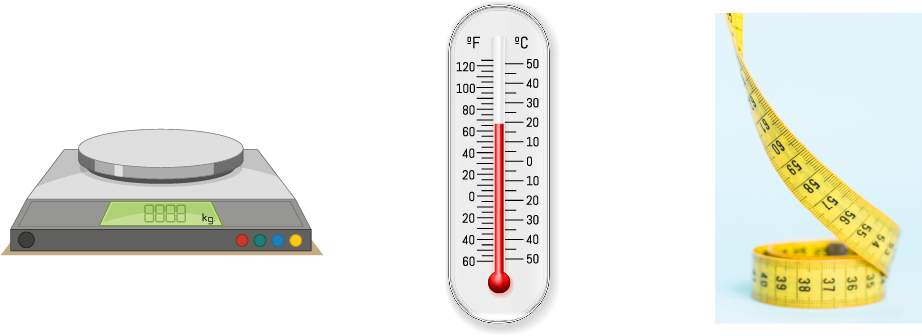
\includegraphics[width=2.60897in,height=1.46587in]{media/image70.png}

O caminho indicado é o de um corredor entre a bilheteria e o início da exposição.
Quanto ele precisará andar para chegar?

\begin{enumerate}
\def\labelenumi{\alph{enumi})}
\item
  8 m.
\item
  10 m.
\item
  12 m.
\item
  14 m.
\end{enumerate}

SAEB: Medir ou comparar perímetro ou área de figuras planas desenhadas em malha quadriculada.
BNCC: EF04MA20 -- Medir e estimar comprimentos (incluindo perímetros), massas e capacidades, utilizando
unidades de medida padronizadas mais usuais, valorizando e respeitando a cultura local.

a) Incorreta. O aluno contou errado a quantidade de quadradinhos.
b) Correta. Paulo deverá andar 5 lados de quadrado. Como cada lado de quadrado possui medida igual a 2 m, ele deverá andar 10 metros.
c) Incorreta. O aluno contou errado a quantidade de quadradinhos.
d) Incorreta. O aluno contou errado a quantidade de quadradinhos.


\subsubsection{2.}\label{section-63}

Observe atentamente as figuras abaixo:

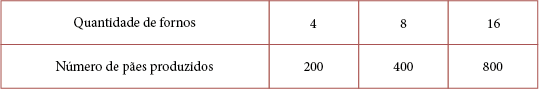
\includegraphics[width=3.39196in,height=2.27520in]{media/image71.png}

Após a análise das figuras, percebe-se que:

\begin{enumerate}
\def\labelenumi{\alph{enumi})}
\item
  a primeira figura é a que possui a maior área.
\item
  a última figura é a que possui a menor área.
\item
  todas as figuras possuem a mesma área.
\item
  todas as figuras possuem áreas diferentes.
\end{enumerate}

SAEB: Resolver problemas que envolvam área de figuras planas
BNCC: EF04MA21 -- Medir, comparar e estimar área de figuras planas desenhadas em malha quadriculada,
pela contagem dos quadradinhos ou de metades de quadradinho, reconhecendo que duas figuras
com formatos diferentes podem ter a mesma medida de área.

a) Incorreta. O aluno contou errado o número de quadradinhos de cada figura.
b) Incorreta. O aluno contou errado o número de quadradinhos de cada figura.
c) Correta. Todas as figuras possuem 6 quadradinhos de área.
b) Incorreta. O aluno contou errado o número de quadradinhos de cada figura.

\subsubsection{3.}\label{section-64}

Maria começou a se arrumar para um passeio com suas amigas na hora em
que, no relógio de seu quarto, o ponteiro menor estava entre o 11 e 12, enquanto o ponteiro maior estava sobre o 7. Ela terminou de se arrumar em 55 minutos. Que horário
o relógio estava marcando nesse segundo momento?

\begin{enumerate}
\def\labelenumi{\alph{enumi})}
\item
  11 horas e 50 minutos.
\item
  12 horas.
\item
  12 horas e 20 minutos.
\item
  12 horas e 30 minutos.
\end{enumerate}

SAEB: Identificar horas em relógios analógicos ou associar horas em relógios analógicos e digitais.
BNCC: EF04MA22 -- Ler e registrar medidas e intervalos de tempo em horas, minutos e segundos em
situações relacionadas ao seu cotidiano, como informar os horários de início e término de realização
de uma tarefa e sua duração.

a) Incorreta. O aluno não soube interpretar o horário no relógio analógico.
b) Incorreta. O aluno trocou o ponteiro das horas com o dos minutos.
c) Incorreta. O aluno trocou o ponteiro das horas com o dos minutos.
d) Correta. O relógio estava marcando 11 horas e 35 minutos. Acrescentando a esse horário 55 minutos, tem-se no relógio 12 horas e 30 minutos.


\section{6. O sistema monetário brasileiro}\label{muxf3dulo-6}

\colorsec{Habilidades do SAEB}

\begin{itemize}
\item Relacionar valores de moedas e/ou cédulas do sistema monetário
brasileiro, com base nas imagens desses objetos.
\item Resolver problemas que envolvam moedas e/ou cédulas do sistema
monetário brasileiro.
\end{itemize}

\colorsec{Habilidade da BNCC}

\begin{itemize}
  \item EF04MA25.
\end{itemize}

\subsection{Conteúdo}\label{conteuxfado-5}
Veja representações das cédulas e das moedas que usamos no Brasil.

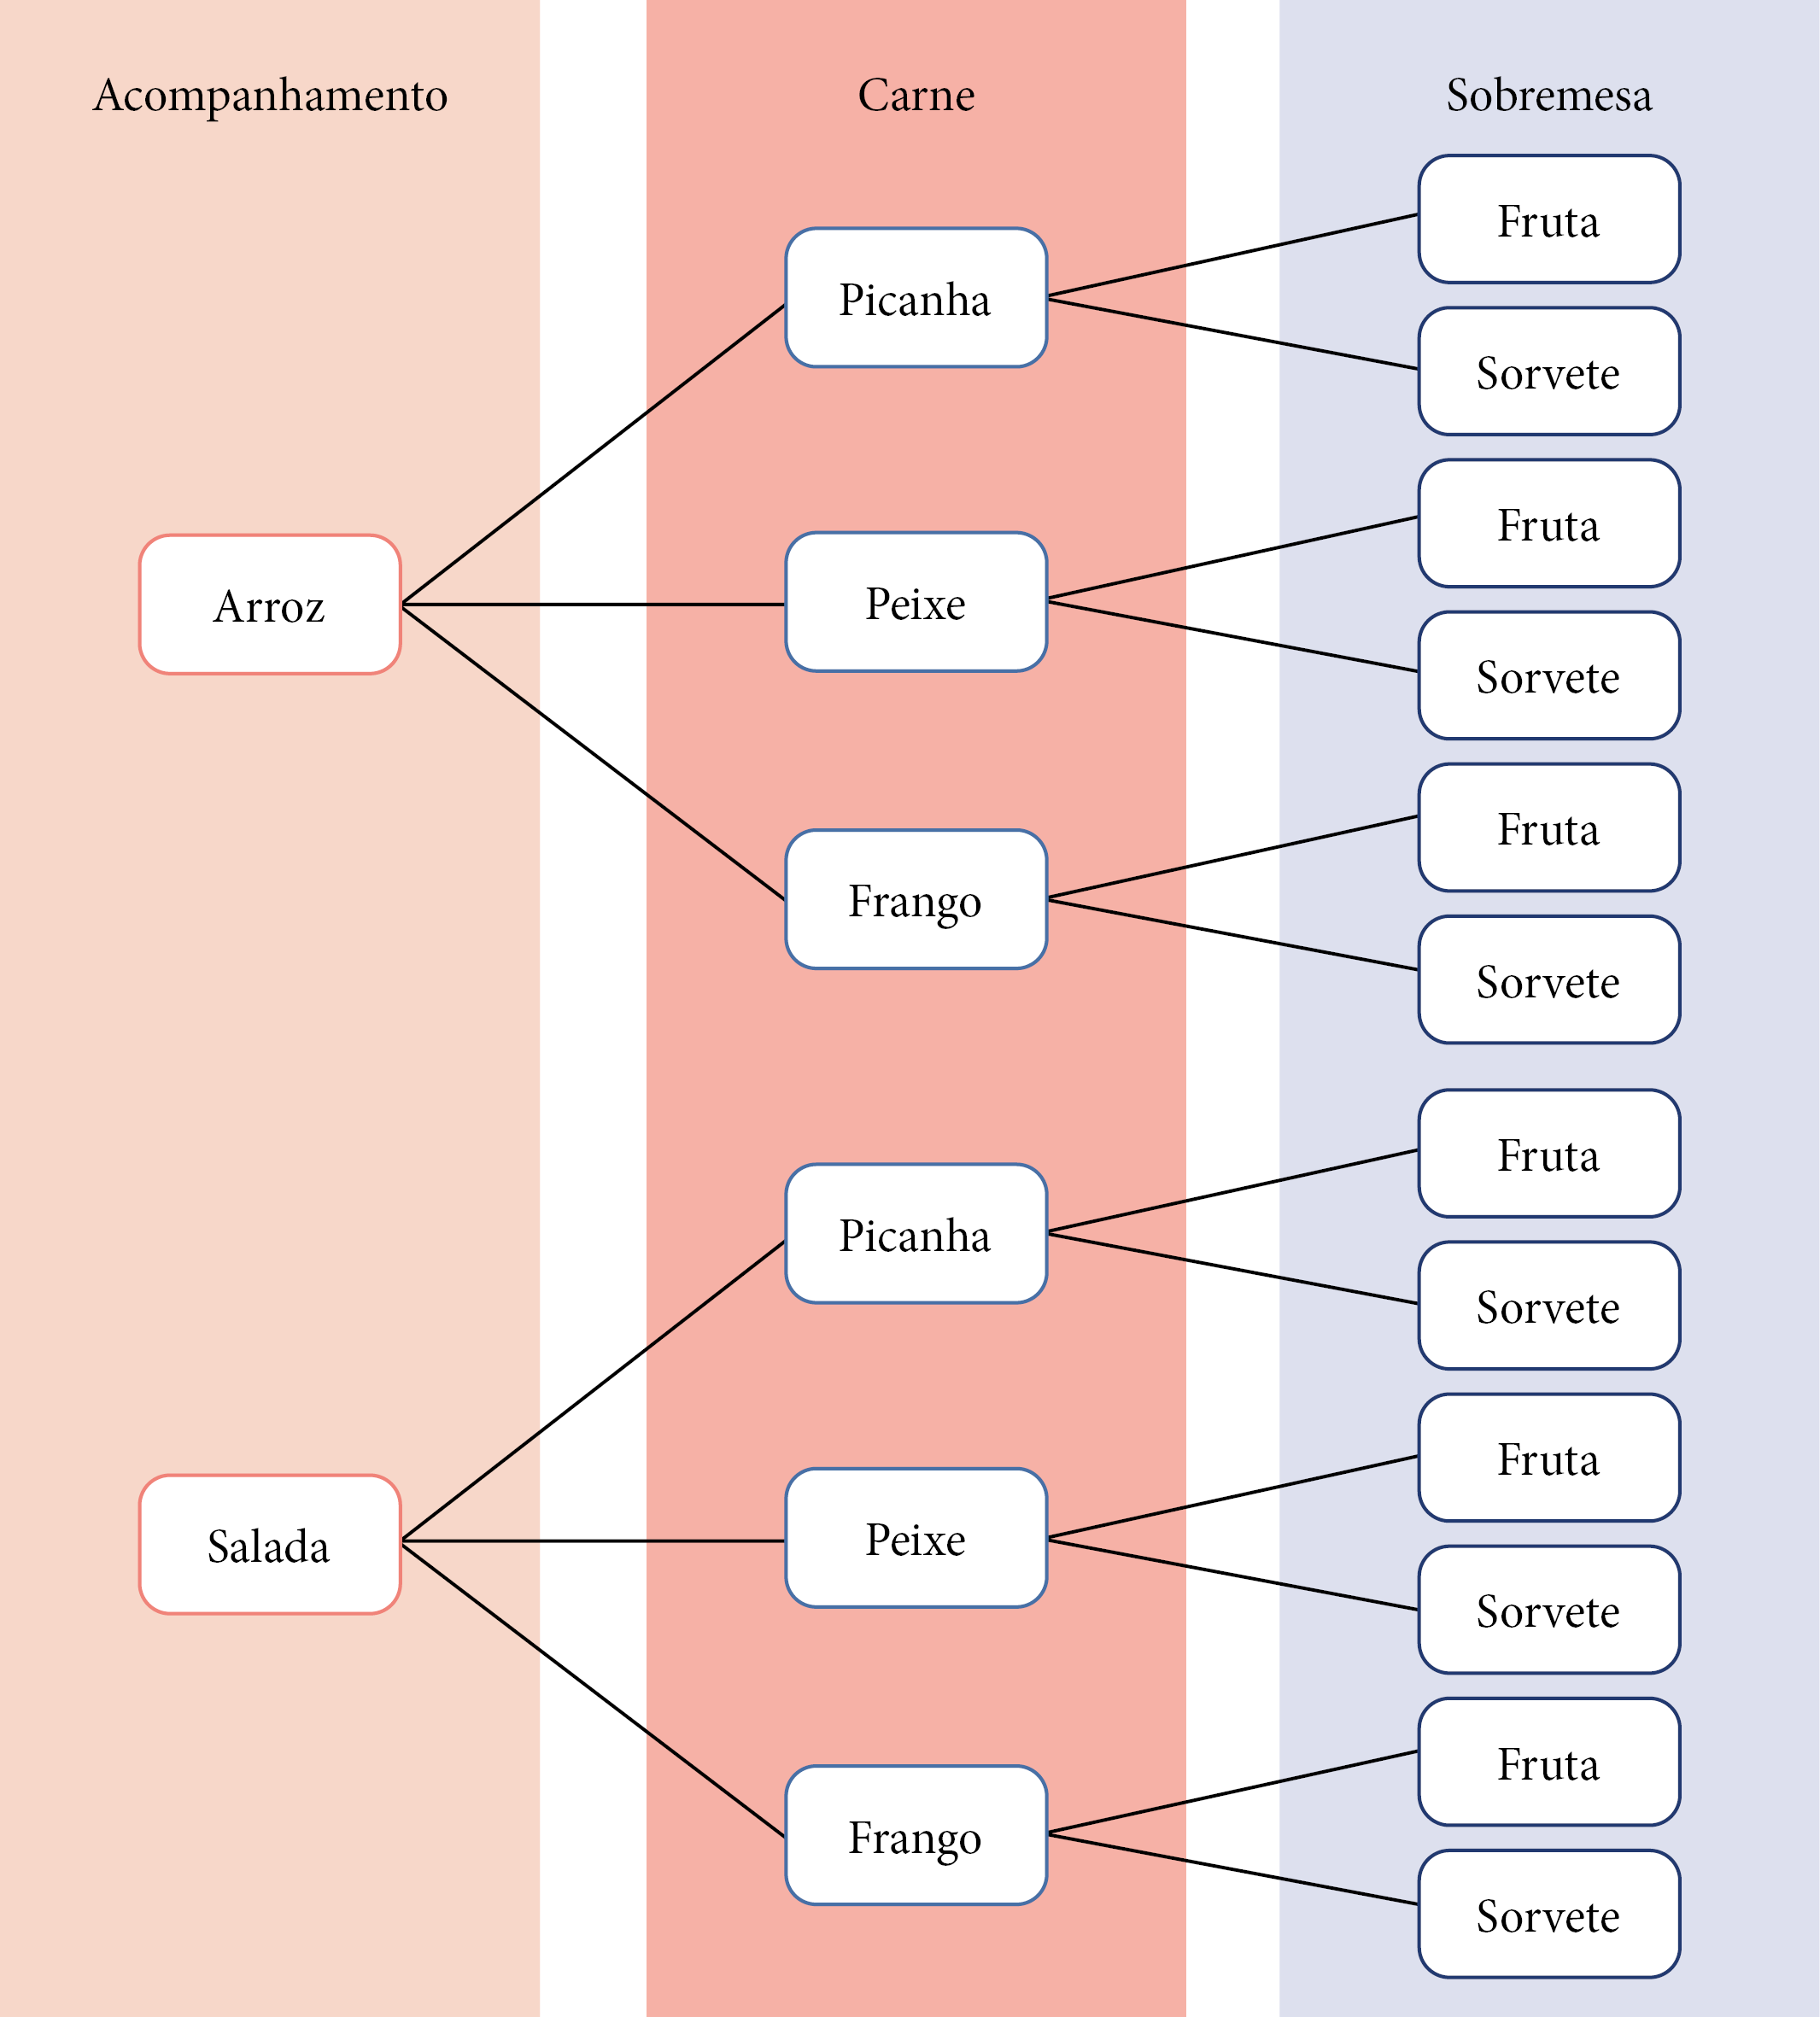
\includegraphics[width=1.80833in,height=1.75637in]{media/image73.png}Moeda
de 5 centavos: R\$ 0,05.

\url{https://img.freepik.com/fotos-gratis/dinheiro-moedas-brasileiras-5-centavos_58702-6209.jpg?w=1060\&t=st=1677437125~exp=1677437725~hmac=c640dd9c5a2963fb4f314f44e074b714cda9416e178bd281b3d494e8262ac50e}

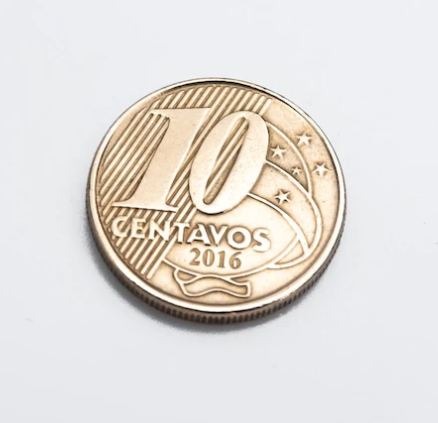
\includegraphics[width=1.50833in,height=1.45668in]{media/image74.png}Moeda
de 10 centavos: R\$ 0,10.

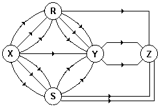
\includegraphics[width=1.52500in,height=1.24749in]{media/image75.png}Moeda
de 25 centavos: R\$ 0,25.

\url{https://img.freepik.com/fotos-gratis/dinheiro-moedas-brasileiras-25-centavos_58702-6230.jpg?w=1060\&t=st=1677437194~exp=1677437794~hmac=db98c5063a731e98b23627749d52c094bab4a2f113240f1f248ee1be7074b235}

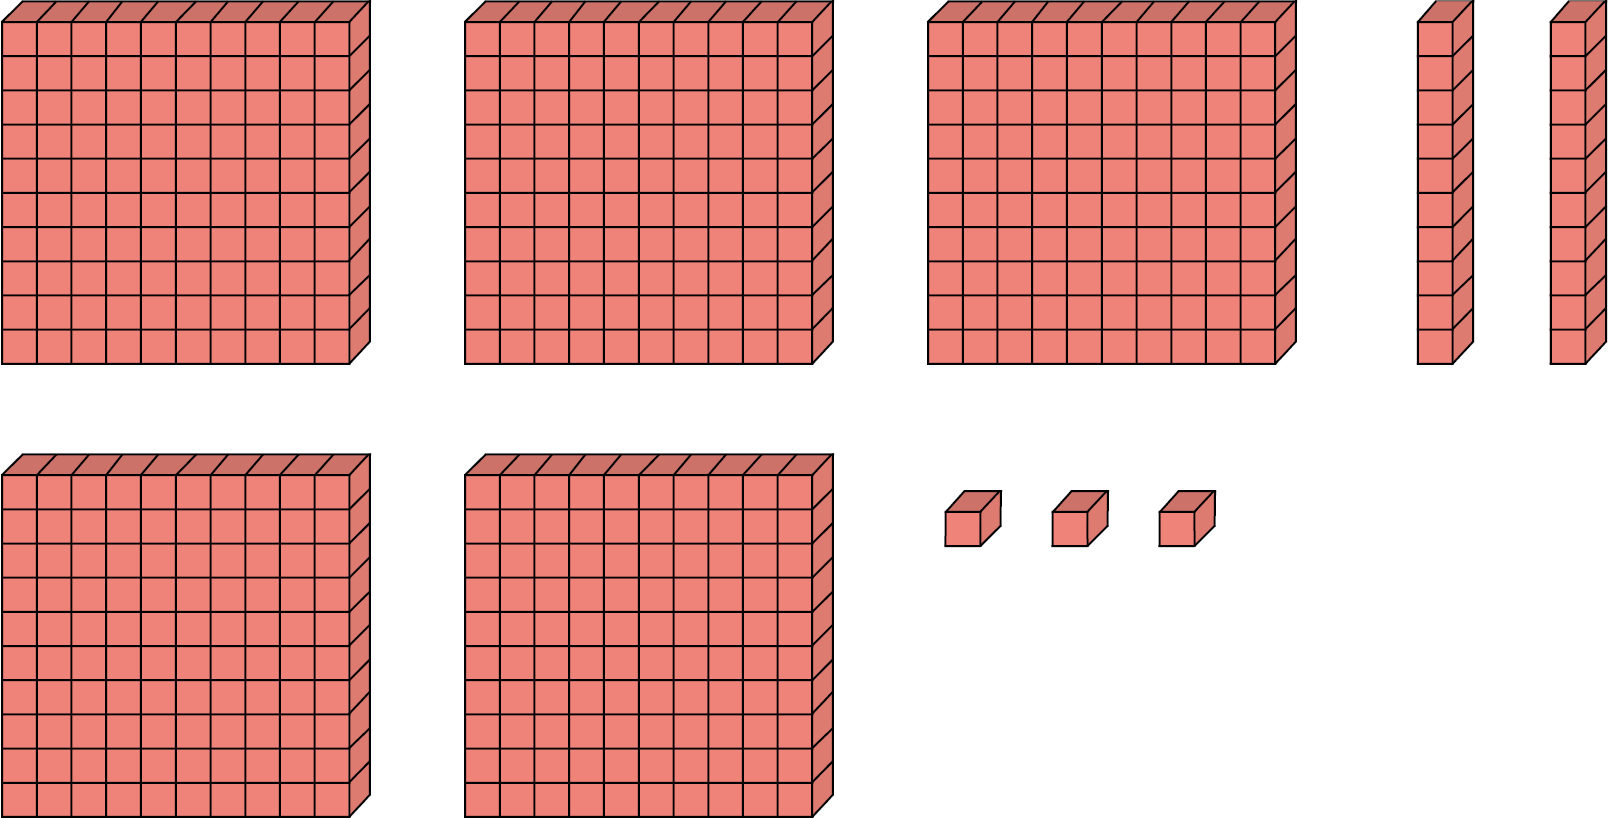
\includegraphics[width=1.56667in,height=1.61849in]{media/image76.png}Moeda
de 50 centavos: R\$ 0,50.

\url{https://img.freepik.com/fotos-gratis/dinheiro-moedas-brasileiras-50-centavos_58702-6291.jpg?w=1060\&t=st=1677437366~exp=1677437966~hmac=a914e13013ee69679658ce52473a57d18d6d23ed6356e75e5d5a34316e88cd82}

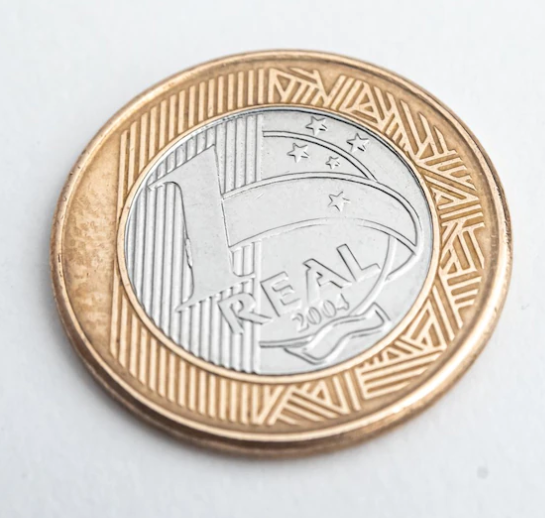
\includegraphics[width=2.11667in,height=2.01180in]{media/image77.png}Moeda
de 1 real: R\$ 1,00.

\url{https://img.freepik.com/fotos-gratis/dinheiro-moedas-brasileiras-1-real_58702-6210.jpg?w=1060\&t=st=1677437258~exp=1677437858~hmac=3314b729d5619da0bffa3b7ce7fe354ae155c324f94ca82e2cb356693ffc25dc}


\includegraphics[width=2.71068in,height=1.97500in]{media/image78.png}
Nota de 2 reais: R\$ 2,00; nota de 5 reais: R\$ 5,00; nota de 10 reais: R\$ 10,00; nota de 20 reais: R\$ 20,00; nota de 50 reais: R\$ 50,00.

\url{https://img.freepik.com/vetores-gratis/ilustracao-gradiente-de-caixa-brasileira_52683-78831.jpg?w=996\&t=st=1677437712~exp=1677438312~hmac=c23ec28122c2591b7b261ceca09eb7c0a64059387f9729dc642986ca98524f1c}
n

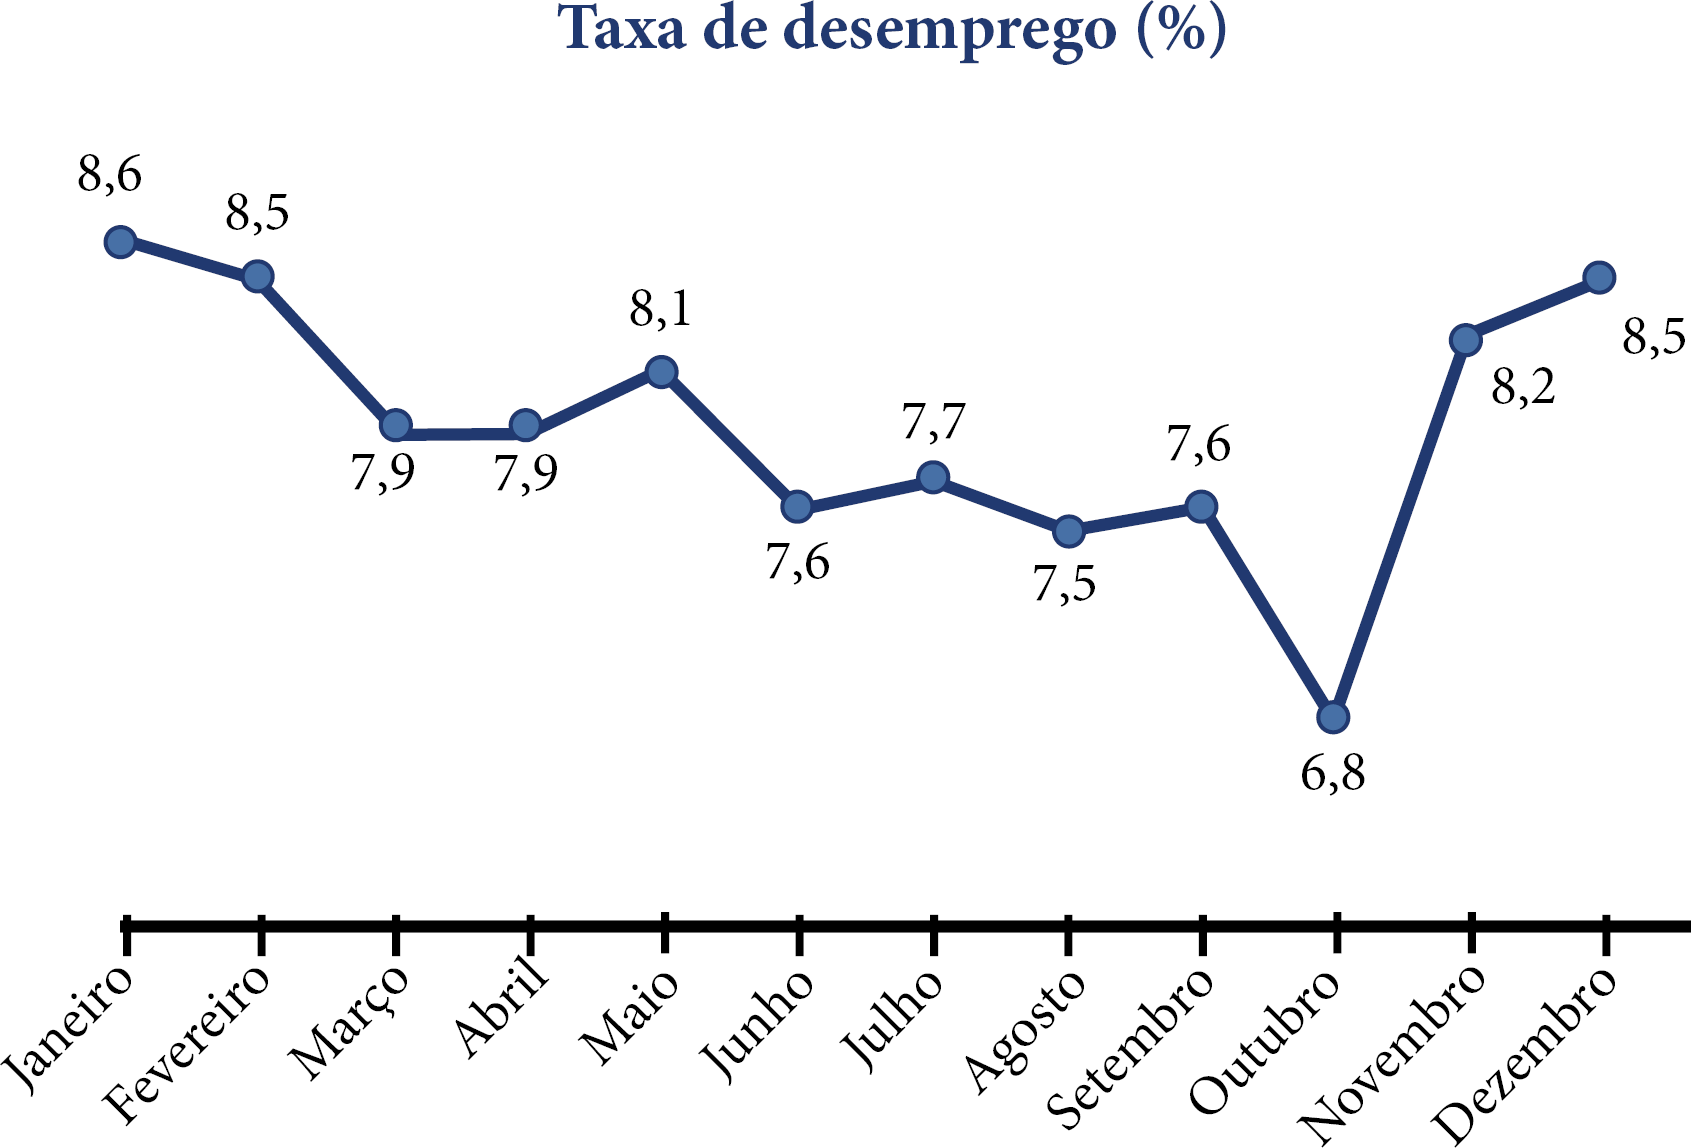
\includegraphics[width=3.18285in,height=1.50833in]{media/image79.png}Nota
de 100 reais R\$ 100,00.

\url{https://img.freepik.com/fotos-premium/cem-reais-contas-dinheiro-brasileiro_499484-1535.jpg?w=1060}


\includegraphics[width=2.68333in,height=1.88913in]{media/image80.png}Nota
de 200 reais: R\$ 200,00.

\subsection{Atividades}\label{atividades-5}

\subsubsection{1.}\label{section-65}

Marta foi à papelaria comprar uma caneta de que estava precisando para
continuar seus estudos. Ela comprou uma caneta que custava 7 reais e 25
centavos. Sabendo-se que ela pagou com uma nota de 10 reais, quais
cédulas e moedas ela recebeu de troco?

Possibilidade de resposta: uma cédula de 2 reais, uma moeda de 50 centavos e uma moeda de 25 centavos.

\subsubsection{2.}\label{section-66}

Caíque economizou muito dinheiro, pois queria comprar um \textit{videogame} usado,
que custava R\$ 2.490,00 à vista. Ele conversou com o vendedor e pediu
um desconto extra e foi atendido com um desconto de R\$ 250,00. Quanto
ele pagou pelo \textit{videogame}?

R\$ 2.490,00 -- R\$ 250,00 = R\$ 2.240,00.

\num{3} Ainda com R\$ 4.000,00 na conta do banco, Ana tinha as seguintes contas para pagar em determinado dia do mês:

\begin{itemize}
  \item Cartão de crédito: R\$ 1.128,00;
  \item Aluguel: R\$ 1.900,00;
  \item \textit{Petshop}: R\$ 480,00;
  \item Clube de assinatura: R\$ 635,00.
\end{itemize}

Ana terá dinheiro suficiente para pagar todas as contas? Explique.

\coment{Ana tem 1.128 + 1.900 + 480 + 635 = 4.143 reais de contas para pagar, mas só tem R\$ 4.000,00 na conta do banco, valor que é 143 reais menor do que o valor de ela precisa.}


\subsubsection{4.}\label{section-68}

Em muitas compras a prazo, é exigida uma entrada que é paga no ato da
compra e o restante do valor pode ser dividido em um número combinado de
parcelas mensais. Veja o exemplo mostrado a seguir.

Compre seu carro com uma entrada de R\$ 35.000,00 e 24
parcelas de R\$ 1.622,00.

Agora, responda ao que se pergunta a seguir.

\begin{enumerate}
\def\labelenumi{\alph{enumi})}
\item
  Qual é o valor que será dividido em 24 vezes?
\end{enumerate}

24 x 1.622 = R\$ 38.928,00.

\begin{enumerate}
\def\labelenumi{\alph{enumi})}
\item
  Qual é o valor que cada parcela terá?
\end{enumerate}

R\$ 1.622,00.

\begin{enumerate}
\def\labelenumi{\alph{enumi})}
\item
  Se à vista a concessionária fornece um desconto de R\$ 4.580,00, quem optar por
  pagar à vista pagará quanto pelo carro?
\end{enumerate}

35.000 + (24 x 1.622) -- 4.580 = R\$ 69.348,00.

\num{5} Responda ao que se pergunta a seguir, utilizando, em cada caso, o maior número possível de cédulas de cada valor.

\begin{escolha}
\item Com cédulas de 20, 10 e 2 reais, como se pode compor o valor R\$ 836,00?
\coment{Quarenta e uma cédulas de 20 reais, uma cédula de 20 reais e três cédulas de 2 reais.}
\item Com cédulas de 200, 50 e 20 reais, como se pode compor o valor R\$ 3.940?
\coment{Dezenove cédulas de 200 reais, duas cédulas de 50 reais e duas cédulas de 20 reais.}
\item Com cédulas de 100, 10 e 5 reais, como se pode compor o valor R\$ 1.735?
\coment{Dezessete cédulas de 100 reais, três cédulas de 10 reais e uma cédula de 5 reais.}

\subsubsection{6.}\label{section-70}

Em um restaurante, dois amigos pediram um prato feito, um prato executivo
e dois refrigerantes. O prato feito custa R\$ 22,00, o executivo custa R\$
28,00 e o refrigerante custa R\$ 6,00. Com três notas de vinte reais, eles
conseguem pagar a conta? Justifique a resposta com cálculos.

22 + 28 + (2 x 6) = R\$ 62,00.
Portanto 3 x 20 reais não serão suficientes para pagar a conta.

\subsubsection{7.}\label{section-71}

Observe alguns preços de uma loja.

\begin{itemize}
  \item \textbf{\textit{Notebook}}: R\$ 3.598,00.
  \item \textbf{\textit{Tablet}}: R\$ 1.680,00.
  \item \textbf{\textit{Smartphone}}: R\$ 2.640,00.
\end{itemize}

Agora, responda ao que se pergunta a seguir.

\begin{enumerate}
\def\labelenumi{\alph{enumi})}
\item
  Quanto uma pessoa gastará se comprar um item de cada?
\end{enumerate}

Deixar espaço em branco equivalente a 3 linhas para a resolução

\begin{enumerate}
\def\labelenumi{\alph{enumi})}
\item
  Quantos reais o \textit{notebook} é mais caro que o \textit{tablet}?
\end{enumerate}

Deixar espaço em branco equivalente a 3 linhas para a resolução

Resposta:

\begin{enumerate}
\def\labelenumi{\alph{enumi})}
\item
  3.598 + 1.680 + 2.640 = R\$ 7.918,00.
\item
  3.598 -- 1.680 = R\$ 1.918,00.
\end{enumerate}

\subsubsection{8.}\label{section-72}

Mariana está pesquisando o preço de alguns itens de que está precisando e chegou aos resultados a seguir.

\begin{itemize}
  \item Cola de bastão: R\$ 0,80.
  \item Rolo de fita adesiva: R\$ 0,50.
  \item Caneta ultrafina: R\$ 0,95.
  \item Borracha branca: R\$ 0,35.
\end{itemize}

Agora, responda ao que se pergunta a seguir.

\begin{enumerate}
\def\labelenumi{\alph{enumi})}
\item
  Qual é a menor quantidade de moedas de 1 real de que ela necessitará para
  pagar por duas unidades de cada item?
\end{enumerate}

\begin{enumerate}
\def\labelenumi{\alph{enumi})}
\item
  Qual é o troco que ele deverá receber nessa situação?
\end{enumerate}

Resposta:

Preço a pagar: 2 x (0,80 + 0,50 + 0,95 + 0,35) = R\$ 5,20. Para esse
valor, ela precisará de 6 moedas de 1 real e terá R\$ 0,80 de troco.

\subsubsection{9.}\label{section-73}

Uma rede de supermercados anunciou uma promoção com os produtos a seguir.

\begin{itemize}
  \item Limpador multiuso: R\$ 3,75.
  \item Amaciante de roupa: R\$ 7,30.
  \item Água sanitária: R\$ 3,25.
  \item Desinfetante: R\$ 3,99.
  \item Desengordurante: R\$ 15,80.
\end{itemize}

Agora, faça o que se pede a seguir.

\begin{enumerate}
\def\labelenumi{\alph{enumi})}
\item
  Escreva como deve ser lido o preço de cada um dos produtos anunciados.
\end{enumerate}

\begin{enumerate}
\def\labelenumi{\alph{enumi})}
\item
  Construa uma sequência decrescente com os preços dos produtos
  anunciados.
\end{enumerate}

\begin{enumerate}
\def\labelenumi{\alph{enumi})}
\item
  Determine quantas notas de 20 reais são necessárias para adquirir uma unidade de
  cada produto anunciado.
\end{enumerate}

\begin{enumerate}
\def\labelenumi{\alph{enumi})}
\item
  Determine qual será o troco na situação apresentada no item anterior.
\end{enumerate}

\begin{enumerate}
\def\labelenumi{\alph{enumi})}
\item
  R\$ 3,75: três reais e setenta e cinco centavos.
\end{enumerate}

R\$ 7,30: sete reais e trinta centavos.

R\$ 3,25: três reais e vinte e cinco centavos.

R\$ 3,99: três reais e noventa e nove centavos.

R\$ 15,80: quinze reais e oitenta centavos.

\begin{enumerate}
\def\labelenumi{\alph{enumi})}
\item
  (15,80; 7,30; 3,99; 3,75; 3,25).
\item
  3,75 + 7,30 + 3,25 + 3,99 + 15,80 = R\$ 34,09; portanto são necessárias duas notas de 20
  reais.
\item
  40 -- 34,09 = R\$ 5,91 de troco.
\end{enumerate}

\subsubsection{10.}\label{section-74}

Valentina vendeu alguns itens que não utilizava mais e como pagamento
recebeu um cheque em que estava escrito: doze mil quatrocentos e
cinquenta e nove reais. Como sua conta estava sem dinheiro algum, ela
resolveu depositar o cheque. No dia seguinte, realizou uma compra no
cartão de débito no valor de RS 12.305,92. Após essa operação qual será o
saldo de Valentina em sua conta bancária?

R\$ 12.459,00 -- R\$ 12.305,92 = R\$ 153,08.

\subsection{Treino}\label{treino-5}

\subsubsection{1.}\label{section-75}

Maria Luísa resolveu trocar com seu primo Francisco as moedas que ganhou de seu avô por notas de
R\$ 2,00. Em seu cofre, havia doze moedas de R\$ 0,50
e oito moedas de R\$ 0,25. Quantas cédulas Maria Luísa recebeu de Francisco?

\begin{enumerate}
\def\labelenumi{\alph{enumi})}
\item
  4.
\item
  6.
\item
  8.
\item
  20.
\end{enumerate}

SAEB: Resolver problemas que envolvam moedas e/ou cédulas do sistema monetário brasileiro.
BNCC: EF04MA25 -- Resolver e elaborar problemas que envolvam situações de compra e venda e formas
de pagamento, utilizando termos como troco e desconto, enfatizando o consumo ético, consciente e
responsável.

a) Correta. (12 x R\$ 0,50) + (8 x R\$ 0,25) = R\$ 6,00 + R\$ 2,00 = R\$ 8,00 = 4 cédulas de R\$ 2,00.
b) Incorreta. O aluno fez a associação errada dos valores com as quantidades.
c) Incorreta. O aluno só calculou o valor que seria trocado.
d) Incorreta. O aluno só calculou a quantidade de moedas sem considerar o valor.


\subsubsection{2.}\label{section-76}

Letícia resolveu arrumar o que estava em sua bolsa e encontrou
os seguintes valores: uma cédula de R\$ 5,00, duas cédulas de R\$ 2,00, uma moeda de R\$ 0,50, uma moeda de R\$ 0,25, três moedas de R\$ 0,10 e duas moedas de R\$ 0,05. No total, Letícia possui

\begin{enumerate}
\def\labelenumi{\alph{enumi})}
\item
  R\$ 9,00.
\item
  R\$ 9,90.
\item
  R\$ 10,10.
\item
  R\$ 10,15.
\end{enumerate}

SAEB: Resolver problemas que envolvam moedas e/ou cédulas do sistema monetário brasileiro.
BNCC: EF04MA25 -- Resolver e elaborar problemas que envolvam situações de compra e venda e formas
de pagamento, utilizando termos como troco e desconto, enfatizando o consumo ético, consciente e
responsável.

a) Incorreta. O aluno se esqueceu de contar as moedas.
b) Incorreta. O aluno não contou todas as moedas.
c) Incorreta. O aluno deixou de contar uma moeda de 5 centavos.
d) Correta. Letícia tem R\$ 9,00 em cédulas e R\$ 1,15 em moedas; portanto, no total, ela
encontrou em sua bolsa R\$ 10,15.

\subsubsection{3.}\label{section-77}

Na lanchonete a que Augusto costuma ir com seus amigos, existe a tabela de preços a seguir.

\begin{longtable}[]{@{}ll@{}}
\toprule
Produto & Valor por unidade\tabularnewline
\midrule
\endhead
Pão de queijo & R\$ 3,00\tabularnewline
Bombom & R\$ 5,00\tabularnewline
Suco & R\$ 6,00\tabularnewline
Sobremesa do dia & R\$ 4,50\tabularnewline
Refrigerante & R\$ 4,50\tabularnewline
Cachorro-quente & R\$ 12,00\tabularnewline
\bottomrule
\end{longtable}

Na última vez em que Augusto foi a esse lugar, ele comprou 4 bombons, 2
sucos e 3 cachorros-quentes. Qual é o valor gasto por Augusto nesse dia?

\begin{enumerate}
\def\labelenumi{\alph{enumi})}
\item
  R\$ 20,00.
\item
  R\$ 23,00.
\item
  R\$ 68,00.
\item
  R\$ 73,00.
\end{enumerate}

SAEB: Resolver problemas que envolvam moedas e/ou cédulas do sistema monetário brasileiro.
BNCC: EF04MA25 -- Resolver e elaborar problemas que envolvam situações de compra e venda e formas
de pagamento, utilizando termos como troco e desconto, enfatizando o consumo ético, consciente e
responsável.

a) Incorreta. O aluno contou apenas os bombons.
b) Incorreta. O aluno errou nos cálculos.
c) Correta. (4 x 5,00) + (2 x 6,00) + (3 x 12,00) = 20,00 + 12,00 + 36,00 = R\$ 68,00.
d) Incorreta. O aluno contou um bombom a mais.


\section{7. Qual é a probabilidade?}\label{muxf3dulo-7}

\colorsec{Habilidades do SAEB}

\begin{itemize}
\item Identificar, entre eventos aleatórios, aqueles que têm menos, maiores ou
iguais chances de ocorrência, sem utilizar frações.
\item Determinar a probabilidade de ocorrência de um resultado em eventos
aleatórios, quando todos os resultados possíveis têm a mesma chance de
ocorrer (equiprováveis).
\end{itemize}

\colorsec{Habilidade da BNCC}

\begin{itemize}
\item EF04MA26.
\end{itemize}

\subsection{Conteúdo}\label{conteuxfado-6}

Probabilidade é a chance de determinado
resultado ocorrer. O número 0 representa ``nenhuma chance'', enquanto o número 1
corresponde a ``chance certa''.

Quando se fala e probabilidade, é importante pensar nos fenômenos aleatórios, ou seja, aqueles cujo resultado não pode ser determinado mesmo se conhecendo todos os resultados possíveis. Por falar nisso, espaço amostral é o conjunto desses resultados.

\subsection{Atividades}\label{atividades-6}

\subsubsection{1.}\label{section-78}

Em um estojo, há 25 lápis coloridos e 18 lápis pretos. Retirando-se, ao
acaso, um lápis desse estojo, o que tem chance maior: retirar um lápis
colorido ou um preto? Justifique sua resposta.

%Deixar espaço em branco equivalente a 3 linhas para a resolução

\coment{Como há mais lápis coloridos do que pretos no estojo, a maior chance,
quando se retira um único lápis desse estojo, é que saia um lápis
colorido.}

\subsubsection{2.}\label{section-79}

Daniel joga um dado honesto. Sobre isso, determine as chances mencionadas a seguir.

\begin{enumerate}
\def\labelenumi{\alph{enumi})}
\item
  Tirar, na face voltada para cima, um número par.
\end{enumerate}

%Deixar espaço em branco equivalente a 2 linhas para a resolução

\begin{enumerate}
\def\labelenumi{\alph{enumi})}
\item
  Tirar, na face voltada para cima, um número ímpar.
\end{enumerate}

%Deixar espaço em branco equivalente a 2 linhas para a resolução

\begin{enumerate}
\def\labelenumi{\alph{enumi})}
\item
  Tirar, na face voltada para cima, um número menor que 3.
\end{enumerate}

%Deixar espaço em branco equivalente a 2 linhas para a resolução

Resposta:

\begin{enumerate}
\def\labelenumi{\alph{enumi})}
\item
  Temos sempre 6 possibilidades de números que podem sair: 1, 2, 3, 4, 5 e 6. Se interessa um número par, há três chances de isso acontecer (2, 4, 6).
\end{enumerate}

\begin{enumerate}
\def\labelenumi{\alph{enumi})}
\item
  Temos sempre 6 possibilidades de números que podem sair: 1, 2, 3, 4, 5 e 6. Se interessa um número ímpar, há três chances de isso acontecer (1, 3, 5).
\end{enumerate}

\begin{enumerate}
\def\labelenumi{\alph{enumi})}
\item
  Temos sempre 6 possibilidades de números que podem sair: 1, 2, 3, 4, 5 e 6. Se interessa um número menor que 3, há duas chances de isso acontecer (1, 2).
\end{enumerate}


\subsubsection{3.}\label{section-80}

Uma sacola escura, que não permite visualizar o que há dentro, contém
50 bolas idênticas, mas de cores diferentes. Sabe-se que 16 são azuis,
18 são pretas, 14 são vermelhas e 2 são amarelas. Calcule as chances de
acontecer o que se prevê a seguir.

\begin{enumerate}
\def\labelenumi{\alph{enumi})}
\item
  Que cor tem mais chance de aparecer quando se retira uma bola ao acaso? Justifique sua resposta.
\end{enumerate}

A maior probabilidade é de sair uma bola preta, porque é a cor que mais aparece na sacola.

\begin{enumerate}
\def\labelenumi{\alph{enumi})}
\item
  Há mais chance de sair um bola azul ou uma bola vermelha da sacola? Justifique sua resposta.
\end{enumerate}

Há mais chance de sair uma bola azul, porque há mais bolas azuis que vermelhas.

\begin{enumerate}
\def\labelenumi{\alph{enumi})}
\item
  Retirando-se uma bola ao acaso, a probabilidade de sair amarela é maior do que a de sair qualquer
  outra cor?
\end{enumerate}

Não, pois a probabilidade de sair uma amarela é a menor entre as
  probabilidades de saírem as outras cores, visto que a quantidade de
  bolas amarelas é a menor de todas.


\subsubsection{4.}\label{section-81}

Lucas tem guardado em uma caixa 16 livros de Matemática, 6 de História e
8 de Geografia. Retirando ao acaso um desses livros da caixa, responda ao que se pergunta a seguir.

\begin{enumerate}
\def\labelenumi{\alph{enumi})}
\item
  Qual livro tem mais chance de sair?
\end{enumerate}

Um livro de Matemática.

\begin{enumerate}
\def\labelenumi{\alph{enumi})}
\item
  Qual livro tem menos chance de sair?
\end{enumerate}

Um livro de História.

\begin{enumerate}
\def\labelenumi{\alph{enumi})}
\item
  Qual é a chance de sair uma livro de Língua Portuguesa?
\end{enumerate}

Não há chance de sair um livro de Língua Portuguesa, porque não há livros desse tipo na caixa.



\subsubsection{5.}\label{section-82}

Na sala em que Clarissa estuda há 26 alunos, dos quais 18 são meninas. A
professora vai escolher um aluno para verificar se esse aluno fez a tarefa.
Uma menina ou um menino é mais provável que vai ser escolhido? Justifique sua resposta.

Deixar espaço em branco equivalente a 3 linhas para a resolução

Resposta:

Total de alunos: 26

Número de meninas: 18
Número de meninos: 26 -- 18 = 8

É mais provável que seja escolhida uma menina.

\subsubsection{6.}\label{section-83}

Uma letra é escolhida ao acaso entre as que formam a palavra
FUNDAMENTAL. É mais provável que a letra escolhida seja uma vogal ou uma consoante?

Deixar espaço em branco equivalente a 3 linhas para a resolução

Resposta:

Total de letras: 11

Consoantes: 7
Vogais: 11 -- 7 = 4

Há mais chance de sair uma consoante.

\subsubsection{7.}\label{section-84}

O baralho convencional é composto de 52 cartas divididas igualmente em quatro
naipes (copas, paus, ouros e espadas). Retirada uma carta ao acaso de um baralho,
qual naipe é mais provável de sair? Justifique sua resposta.

Como são 52 cartas divididas igualmente em quatro naipes, a chance de sair qualquer um dos naipes é sempre a mesma; portanto não há um naipe mais provável.

\subsubsection{8.}\label{section-85}

Vítor quer escolher um número para sua camiseta do time de futebol e ele
pode escolher qualquer número de 1 a 25. Quantas chances ele tem de
escolher um número maior que 8 e menor que 18?

Total de números: 25
Total de números que interessam: 9
Há, portanto, nove chances de sair um número maior que 8 e menor que 18.

\subsubsection{9.}\label{section-86}

Os 500 estudantes de um colégio responderam a uma pergunta sobre a
área de conhecimento preferida, entre Exatas, Humanas e
Biológicas. As respostas foram computadas e alguns dados foram colocados
na tabela a seguir.

\Paulo A tabela não veio certo. Checar o original. Mas não colocar a coluna de total.
\begin{longtable}[]{@{}ll@{}}
\toprule
Área & Sexo\tabularnewline
& Masculino (M)\tabularnewline
Exatas (E) & 120\tabularnewline
Humanas (H) & 45\tabularnewline
Biológicas (B) & 100\tabularnewline
Total & 265\tabularnewline
\bottomrule
\end{longtable}

Um estudante é escolhido ao acaso. Determine a probabilidade de esse
estudante preferir Humanas.

Deixar espaço em branco equivalente a 3 linhas para a resolução.

Resposta:

Total de estudantes: 500
Preferência por humanas: 125
Há 125 chances em 500 de o estudante escolhido ao caso preferir Humanas.

\subsubsection{10.}\label{section-87}

Carlos possui duas urnas com bolas que só são diferenciadas pela cor. A
distribuição das bolas nas urnas por cor se encontra na tabela a
seguir.

\begin{longtable}[]{@{}lll@{}}
\toprule
Cor & Urna 1 & Urna 2\tabularnewline
\midrule
\endhead
Amarela & 4 & 0\tabularnewline
Azul & 3 & 1\tabularnewline
Branca & 2 & 2\tabularnewline
Verde & 1 & 3\tabularnewline
Vermelha & 0 & 4\tabularnewline
\bottomrule
\end{longtable}

Ele vai colocar todas as bolas dessas duas urnas em uma única urna 3. Em
seguida retirará uma bola, ao acaso, dessa terceira urna. Qual é o total de possibilidades e quantas chances ele tem de tirar uma bola verde?

Total de bolas: 20 (possibilidades).
Bolas verdes: 4 (chances).


\subsection{Treino}\label{treino-6}

\subsubsection{1.}\label{section-88}

Mateus precisa ir ao dentista na próxima semana, sem ser um dia de final de semana. Escolhendo ao acaso um dia
qualquer da semana para ir ao dentista, qual é a probabilidade de Mateus
escolher uma quinta-feira?

\begin{enumerate}
\def\labelenumi{\alph{enumi})}
\item
  1 chance em sete.
\item
  2 chances em sete.
\item
  1 chance em cinco.
\item
  2 chances em cinco.
\end{enumerate}

SAEB: Identificar, entre eventos aleatórios, aqueles que têm menos, maiores ou iguais chances de ocorrência, sem utilizar frações.
BNCC: EF04MA26 -- Identificar, entre eventos aleatórios cotidianos, aqueles que têm maior chance de
ocorrência, reconhecendo características de resultados mais prováveis, sem utilizar frações.

a) Incorreta. Não podem ser contados o sábado e domingo.
b) Incorreta. A chance é sempre apenas uma, porque se trata somente da quinta-feira.
c) Correta. Entre os cinco dias possíveis, só a quinta-feira seria escolhida.
d) Incorreta. A chance é sempre apenas uma, porque se trata somente da quinta-feira.

\subsubsection{2.}\label{section-89}

Em determinado momento, um restaurante está com 28 clientes e 7
garçons. Sobre essa situação, pode-se afirmar corretamente que

\begin{enumerate}
\def\labelenumi{\alph{enumi})}
\item
  há mais garçons que clientes.
\item
  é mais provável escolher um garçom ao acaso.
\item
  é mais provável escolher um cliente ao acaso.
\item
  há chances iguais de ser escolhido ao acaso um cliente ou um garçom.
\end{enumerate}

SAEB: Identificar, entre eventos aleatórios, aqueles que têm menos, maiores ou iguais chances de ocorrência, sem utilizar frações.
BNCC: EF04MA26 -- Identificar, entre eventos aleatórios cotidianos, aqueles que têm maior chance de
ocorrência, reconhecendo características de resultados mais prováveis, sem utilizar frações.

a) Incorreta. Há 28 clientes, e apenas 7 garçons.
b) Incorreta. É mais provável escolher um cliente, já que os clientes estão em maior número.
c) Correta. Como há mais clientes que garçons no restaurante, é mais provável que seja escolhido um cliente
d) Incorreta. As chances não são iguais, porque há números diferentes de clientes ou garçons.

\subsubsection{3.}\label{section-90}

Uma estação de rádio está promovendo um concurso que funciona da seguinte maneira: cada vez que um ouvinte acerta qual é a música mais tocada do dia, ganha um cupom para o sorteio final. Veja, a seguir, quantos cupons alguns ouvintes conseguiram ganhar.

\begin{itemize}
  \item Rogéria: 12 cupons;
  \item Paulo: 21 cupons;
  \item Márcia: 29 cupons;
  \item Carlos: 18 cupons.
\end{itemize}

Se todos esses cupons forem colocados em uma urna, da qual será sorteado uma única vez um único cupom, qual dessas pessoas tem mais chance de ser sorteada?

\begin{enumerate}
\def\labelenumi{\alph{enumi})}
\item
  Carlos.
\item
  Márcia.
\item
  Paulo.
\item
  Rogéria.
\end{enumerate}

SAEB: Identificar, entre eventos aleatórios, aqueles que têm menos, maiores ou iguais chances de ocorrência, sem utilizar frações.
BNCC: EF04MA26 -- Identificar, entre eventos aleatórios cotidianos, aqueles que têm maior chance de
ocorrência, reconhecendo características de resultados mais prováveis, sem utilizar frações.

a) Incorreta. Carlos é terceiro com mais chances.
b) Correta. Márcia tem mais cupons que os outros; portanto é a que tem mais chance de ser sorteada.
c) Incorreta. Paulo é o segundo com mais chances.
d) Incorreta. Rogério é a quarta com mais chances.

\section{8. Dados estatísticos\label{muxf3dulo-8}

\colorsec{Habilidades do SAEB}

\begin{itemize}
\item Ler/identificar ou comparar dados estatísticos expressos em tabelas
(simples ou de dupla entrada).
\item Ler/identificar ou comparar dados estatísticos expressos em gráficos
(barras simples ou agrupadas, colunas simples ou agrupadas, pictóricos
ou de linhas).
\item Resolver problemas que envolvam dados apresentados tabelas (simples ou
de dupla entrada) ou gráficos estatísticos (barras simples ou agrupadas,
colunas simples ou agrupadas, pictóricos ou de linhas).
\end{itemize}

\colorsec{Habilidade da BNCC}

\begin{itemize}
\item EF04MA27.
\end{itemize}

\subsection{Conteúdo}\label{conteuxfado-7}

Veja, a seguir, alguns tipos de gráfico mais utilizados em estatística.

\begin{itemize}
\item
  Gráfico de colunas ou barras.
\end{itemize}

Fazer a figura abaixo nos moldes do projeto.

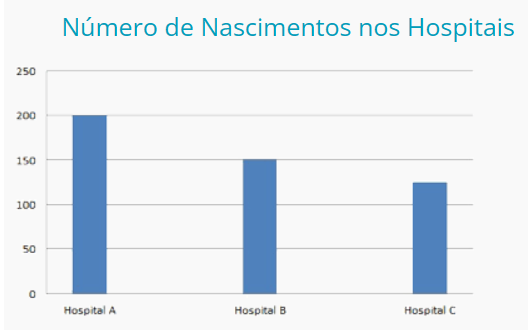
\includegraphics[width=2.58333in,height=1.61458in]{media/image91.png}

\begin{itemize}
\item
  Pictograma.
\end{itemize}

Fazer a figura abaixo nos moldes do projeto.

Além disso ao invés de raparigas colocar meninas e no lugar de rapazes
colocar meninos.

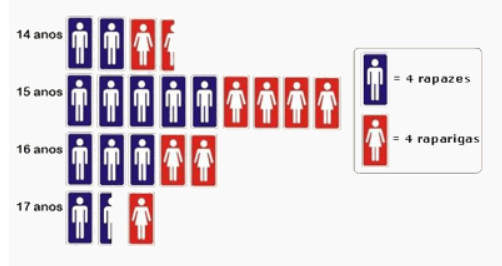
\includegraphics[width=4.18370in,height=2.21686in]{media/image92.png}

\begin{itemize}
\item
  Gráfico de linhas.
\end{itemize}

Fazer a figura abaixo nos moldes do projeto.

Retirar da legenda o nome das emissoras e colocar A, B, C e D.

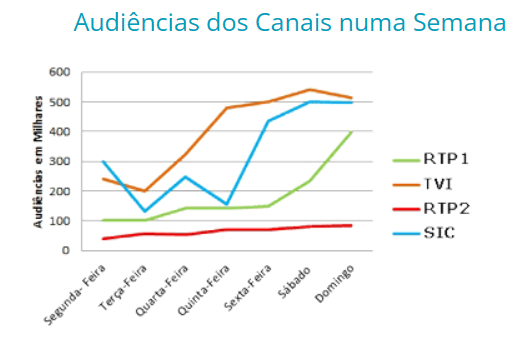
\includegraphics[width=3.19872in,height=2.19483in]{media/image93.png}

\begin{itemize}
\item
  Gráfico de setores.
\end{itemize}

Fazer a figura abaixo nos moldes do projeto.

No lugar de autocarro colocar ônibus

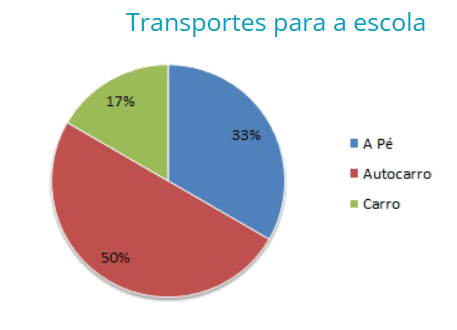
\includegraphics[width=2.42308in,height=1.74971in]{media/image94.png}

\subsection{Atividades}\label{atividades-7}

\subsubsection{1.}\label{section-91}

A tabela a seguir foi construída por uma escola com a finalidade de agrupar os
dados sobre a quantidades de alunos em alguns anos e o período em que
estudam. Observe.

\begin{longtable}[]{@{}lllll@{}}
\toprule
& 6º & 7º & 8º & 9º\tabularnewline
\midrule
\endhead
Período da manhã & 35 & 65 & 72 & 92\tabularnewline
Período da tarde & 54 & 43 & 48 & 43\tabularnewline
\bottomrule
\end{longtable}

Quantos alunos o 6º ano do período da tarde tem a menos que o 9º
ano do período da manhã?

Deixar espaço de 3 linha para resposta

Resposta:

92 -- 54 = 38. O 6º ano do períoda da tarde tem 38 alunos a
menos que o 9º do período da manhã.

\subsubsection{2.}\label{section-92}

A OMS (Organização Mundial de Saúde) realizou uma pesquisa sobre o
consumo diário de água e os dados foram apresentados no gráfico a seguir.

Produzir uma figura semelhante a essa.

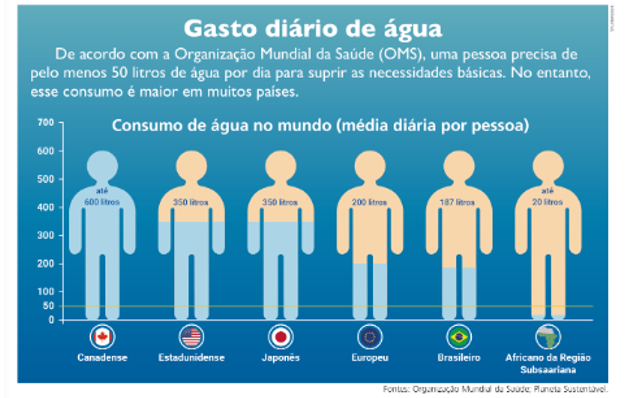
\includegraphics[width=5.22545in,height=3.31695in]{media/image95.png}

Analisando-se atentamente o gráfico, qual é a diferença entre o
consumo diário de um europeu e de um brasileiro?

Deixar espaço de 3 linha para resposta

Resposta:

200 -- 187 = 13 litros.

\subsubsection{3.}\label{section-93}

Após todas as rodadas de um campeonato de futebol, os organizadores
apresentaram o gráfico a seguir sobre o número de pontos ganhos por cada
time.

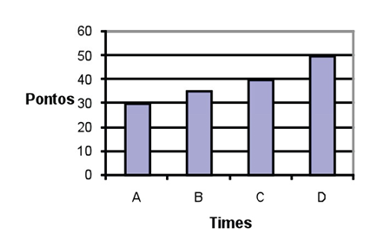
\includegraphics[width=3.19194in,height=2.04184in]{media/image96.png}

Observando atentamente o gráfico, podemos concluir que o time B fez

\begin{enumerate}
\def\labelenumi{\alph{enumi})}
\item
  exatamente 50 pontos.
\item
  mais do que 40 pontos.
\item
  menos do que 25 pontos.
\item
  mais do que 30 pontos.
\end{enumerate}

O time B fez mais do que 30 pontos durante esse campeonato.

\subsubsection{4.}\label{section-94}

Em uma empresa de doces, resolveu-se contratar um matemático que realizasse uma
pesquisa para verificar o tipo preferido de sobremesa das pessoas que
frequentavam determinado supermercado. Os entrevistados poderiam dar
apenas uma resposta entre as oferecidas na pesquisa. Após contagem dos
votos sobre a preferência, o matemático apresentou o gráfico a seguir
para a empresa que o contratou.

\begin{longtable}[]{@{}ll@{}}
\toprule
Sobremesa & Total de votos\tabularnewline
\midrule
\endhead
Pudim & 35\tabularnewline
Sorvete & 20\tabularnewline
Doce de leite & 22\tabularnewline
Goiabada com queijo & 10\tabularnewline
Salada de frutas & 13\tabularnewline
\bottomrule
\end{longtable}

Analisando o gráfico apresentado, responda ao que se pergunta a seguir.

\begin{enumerate}
\def\labelenumi{\alph{enumi})}
\item
  Qual foi a sobremesa menos votada?
\end{enumerate}

Deixar espaço em branco equivalente a 1 linhas para a resolução

\begin{enumerate}
\def\labelenumi{\alph{enumi})}
\item
  Qual foi a sobremesa mais votada?
\end{enumerate}

Deixar espaço em branco equivalente a 1 linhas para a resolução

\begin{enumerate}
\def\labelenumi{\alph{enumi})}
\item
  Como fica uma sequência crescente dos números apresentados na tabela?
\end{enumerate}

Deixar espaço em branco equivalente a 1 linhas para a resolução

\begin{enumerate}
\def\labelenumi{\alph{enumi})}
\item
  Após construir a sequência crescente, qual número ficou na posição
  central? A que sobremesa ele corresponde?
\end{enumerate}

Deixar espaço em branco equivalente a 1 linhas para a resolução

Resposta:

\begin{enumerate}
\def\labelenumi{\alph{enumi})}
\item
  A sobremesa menos votada foi a goiabada com queijo.
\item
  A sobremesa mais votada foi o pudim.
\item
  (10; 13; 20; 22; 35).
\item
  O número que ocupa a posição central na sequência é o 20, que corresponde ao sorvete.
\end{enumerate}

\subsubsection{5.}\label{section-95}

O professor de Educação Física apresentou os dados da quantidade de gols
marcados pelos 4 times que dispuraram o campeonato de futebol da escola no ano
corrente. Analise o gráfico e responda ao que se pergunta a seguir.


\includegraphics[width=3.30769in,height=1.97201in]{media/image97.png}

\begin{enumerate}
\def\labelenumi{\alph{enumi})}
\item
  Qual turma fez a maior quantidade de gols? Qual foi a quantidade?
\end{enumerate}

Deixar espaço em branco equivalente a 1 linhas para a resolução

\begin{enumerate}
\def\labelenumi{\alph{enumi})}
\item
  Quais turmas fizeram um número de gols maior que 6?
\end{enumerate}

Deixar espaço em branco equivalente a 1 linhas para a resolução

\begin{enumerate}
\def\labelenumi{\alph{enumi})}
\item
  Qual turma fez a menor quantidade de gols?
\end{enumerate}

Deixar espaço em branco equivalente a 1 linhas para a resolução

Resposta:

\begin{enumerate}
\def\labelenumi{\alph{enumi})}
\item
  A turma que fez a maior quantidade de gols foi a B, com 9 gols.
\item
  As turmas que fizeram um número de gols maior que 6 foram as turmas B
  e D.
\item
  A turma C foi a que fez a menor quantidade de gols, pois marcou apenas
  2 vezes.
\end{enumerate}

\subsubsection{6.}\label{section-96}

A tabela a seguir mostra parte do cadastro de uma escola.

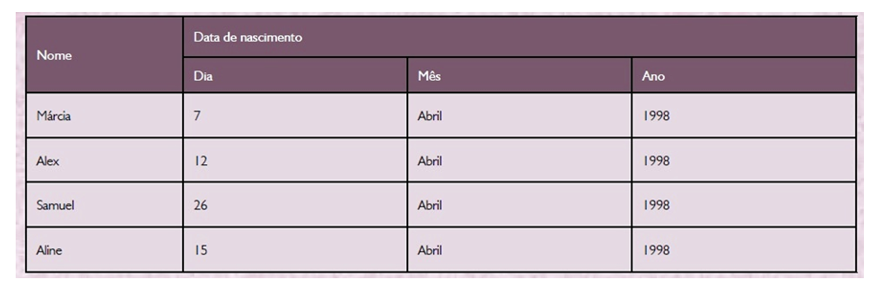
\includegraphics[width=5.90556in,height=1.93264in]{media/image98.png}

%Tabela não deve ter essa cor, nem esse tamanho de espaço de célula e os
dados devem estar centralizados.

Esse são os dados sobre o nascimento dos pais de quatro alunos da sala
de João. Analisando os dados, podemos perceber que a pessoa mais jovem,
entre as apresentadas na tabela, é

\begin{enumerate}
\def\labelenumi{\alph{enumi})}
\item
  Márcia.
\item
  Alex.
\item
  Samuel.
\item
  Aline.
\end{enumerate}

Como todos nasceram em abril do mesmo ano, a pessoa mais jovem será
aquele que nasceu no maior valor que representa o dia. Sendo assim,
o mais jovem é Samuel.

\subsubsection{7.}\label{section-97}

O governo realizou uma pesquisa sobre o número de queimadas que
ocorreram na Amazônia de 2007 a 2020. Analise o gráfico. Depois, faça o que se pede a seguir.

%Produzir uma figura semelhante a essa.

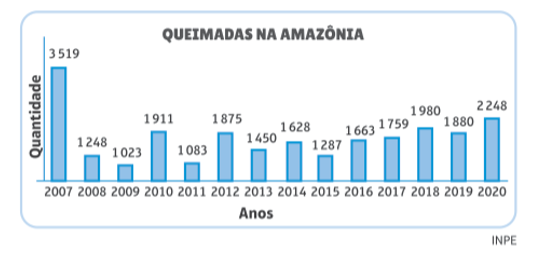
\includegraphics[width=3.71154in,height=1.76937in]{media/image99.png}

\begin{enumerate}
\def\labelenumi{\alph{enumi})}
\item
  Pesquise o significado da sigla INPE, que aparece como fonte dos dados,
  e anote seu significado.
\end{enumerate}

Deixar espaço de 2 linha para resposta

\begin{enumerate}
\def\labelenumi{\alph{enumi})}
\item
  Escreva por extenso o ano em que mais ocorreram queimadas na Amazônia.
\end{enumerate}

Deixar espaço de 1 linha para resposta

\begin{enumerate}
\def\labelenumi{\alph{enumi})}
\item
  Determine os anos em que apareceu um número inferior a 1.500 queimadas na
  Amazônia.
\end{enumerate}

Deixar espaço de 2 linha para resposta

Resposta:

\begin{enumerate}
\def\labelenumi{\alph{enumi})}
\item
  INPE: Instituro Nacional de Pesquisas Espaciais.
\item
  Dois mil e sete foi o ano que apresentou a maior quantidade de
  queimadas na Amazônia.
\item
  2008; 2009; 2011; 2013; 2015.
\end{enumerate}

\subsubsection{8.}\label{section-98}

Os dados fornecidos na tabela a seguir começaram ser passados para um
gráfico pictórico.

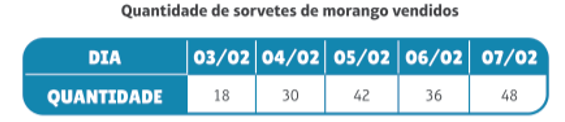
\includegraphics[width=3.47436in,height=0.75022in]{media/image100.png}

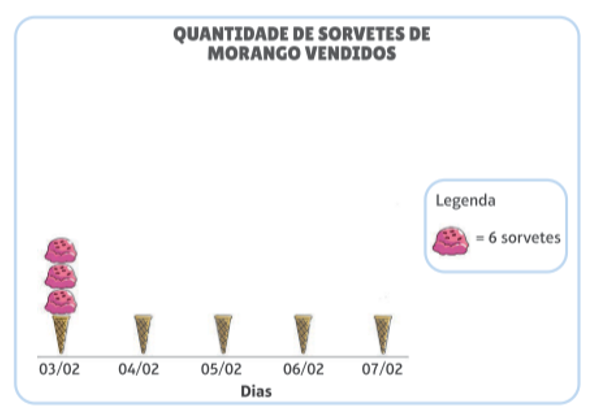
\includegraphics[width=3.86538in,height=2.63899in]{media/image101.png}

Utilizando os dados da tabela e a legenda que o gráfico fornece,
complete o gráfico desenhando as bolas de sorvete que faltam.

Resposta:

04/02: 5 bolas de sorvete.
05/02: 7 bolas de sorvete.
06/02: 6 bolas de sorvete.
07/02: 8 bolas de sorvete.

\subsubsection{9.}\label{section-99}

Utilizando conceitos modernos de educação, a professora de Leonardo
pediu que os alunos da turma realizassem uma pesquisa com 50 pessoas acerca da
preferência deles sobre determinados esportes. Sendo que cada pessoa
escolheu uma única opção, os dados da pesquisa foram colocados na tabela
a seguir.

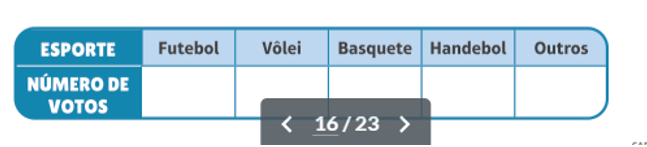
\includegraphics[width=5.39213in,height=1.22511in]{media/image102.png}

Em seguida a professora pediu que os alunos contruíssem um gráfico de
colunas para representar os números da tabela. Construa o gráfico pedido
e ajude Leonardo a concluir a tarefa.

Deixar espaço em branco equivalente a 10 linhas para a resolução

\subsubsection{10.}\label{section-100}

Vanessa tem o hábito de realizar corridas diárias e construiu o seguinte
gráfico de barras com relação à distância percorrida em alguns dias. Observe atentamente o gráfico e responda ao que se pergunta a seguir.

\includegraphics[width=5.22545in,height=2.25853in]{media/image103.png}

\begin{enumerate}
\def\labelenumi{\alph{enumi})}
\item
  Em quais dias da semana ela percorreu a mesma distância?
\end{enumerate}

Deixar espaço em branco equivalente a 1 linhas para a resolução

\begin{enumerate}
\def\labelenumi{\alph{enumi})}
\item
  Quantos quilômetros ela percorreu na sexta-feira?
\end{enumerate}

Deixar espaço em branco equivalente a 1 linhas para a resolução

\begin{enumerate}
\def\labelenumi{\alph{enumi})}
\item
  Em que dia ela percorreu exatamente 10 quilômetros?
\end{enumerate}

Deixar espaço em branco equivalente a 1 linhas para a resolução

\begin{enumerate}
\def\labelenumi{\alph{enumi})}
\item
  Quantos quilômetros, no total, ela percorreu nesses dias apresentados
  no gráfico?
\end{enumerate}

Deixar espaço em branco equivalente a 1 linhas para a resolução

Resposta:

\begin{enumerate}
\def\labelenumi{\alph{enumi})}
\item
  Na segunda-feira e na quinta-feira, ela percorreu a mesma distância: 14 km.
\item
  Na sexta-feira, ela percorreu 16 km.
\item
  Na quarta-feira, ela percorreu 10 km.
\item
  16 + (2 x 14) + 10 + 12 = 16 + 28 + 10 +12 = 66 km.
\end{enumerate}

\subsection{Treino}\label{treino-7}

\subsubsection{1.}\label{section-101}

Pelas regras de um processo seletivo, o candidato que será aprovado será
aquele que tirar todas as notas acima de 30 e, além disso, obtiver o maior
número de notas iguais. As notas de 4 candidatos foram colocadas na
tabela a seguir.

\begin{longtable}[]{@{}lllll@{}}
\toprule
Candidato & Português & Matemática & Direito &
Informática\tabularnewline
\midrule
\endhead
A & 33 & 33 & 33 & 34\tabularnewline
B & 32 & 39 & 32 & 40\tabularnewline
C & 24 & 37 & 40 & 42\tabularnewline
D & 36 & 16 & 26 & 40\tabularnewline
\bottomrule
\end{longtable}

Segundo as regras do concurso, o que será aprovado é o candidato

\begin{enumerate}
\def\labelenumi{\alph{enumi})}
\item
  A.
\item
  B.
\item
  C.
\item
  D.
\end{enumerate}

SAEB: Ler/identificar ou comparar dados estatísticos expressos em tabelas (simples ou de dupla entrada).
BNCC: EF04MA27 -- Analisar dados apresentados em tabelas simples ou de dupla entrada e em gráficos de
colunas ou pictóricos, com base em informações das diferentes áreas do conhecimento, e produzir
texto com a síntese de sua análise.
a) Correta. O candidato A teve todas as notas acima de 30 e é o que teve mais notas iguais.
b) Incorreta. O candidato não teve o maior número de notas iguais, apesar de todas serem acima de 30.
c) Incorreta. O candidato tem uma nota abaixo de 30.
d) Incorreta. O candidato tem duas notas abaixo de 30.


\subsubsection{2.}\label{section-102}

Uma escola fez um levantamente sobre a quantidade de alunos em dois anos
do Ensino Fundamental. Os dados foram apresentados no gráfico a seguir.

%Construir um gráfico como o abaixo na formatação do projeto

\includegraphics[width=2.89744in,height=1.52156in]{media/image104.png}

Quantos alunos o 4º ano tem no total?

\begin{enumerate}
\def\labelenumi{\alph{enumi})}
\item
  60.
\item
  86.
\item
  91.
\item
  150.
\end{enumerate}

SAEB: Ler/identificar ou comparar dados estatísticos expressos em tabelas (simples ou de dupla entrada).
BNCC: EF04MA27 -- Analisar dados apresentados em tabelas simples ou de dupla entrada e em gráficos de
colunas ou pictóricos, com base em informações das diferentes áreas do conhecimento, e produzir
texto com a síntese de sua análise.
a)  Correta. O número total de alunos do 4º ano é dado por esta conta: 32 + 29 + 25 = 86.
b)  Incorreta. O aluno somou 4º e 5º anos da turma A.
c)  Incorreta. O aluno somou os alunos de 5º ano.
d)  Incorreta. O aluno somou a quantidade total de alunos da escola.

\subsubsection{3.}\label{section-103}

Uma loja de brinquedos efetuou uma pesquisa em determinado dia para
saber a faixa etária das crianças que visitaram a loja e os dados foram
colocados no gráfico a seguir.

\includegraphics[width=3.77564in,height=1.60972in]{media/image105.png}

Pode-se afirmar que o total de crianças
de 7 a 12 anos que visitaram a loja é de

\begin{enumerate}
\def\labelenumi{\alph{enumi})}
\item
  7.
\item
  12.
\item
  16.
\item
  21.
\end{enumerate}

SAEB: Ler/identificar ou comparar dados estatísticos expressos em tabelas (simples ou de dupla entrada).
BNCC: EF04MA27 -- Analisar dados apresentados em tabelas simples ou de dupla entrada e em gráficos de
colunas ou pictóricos, com base em informações das diferentes áreas do conhecimento, e produzir
texto com a síntese de sua análise.

a)  Incorreta. O aluno considerou as crianças de 4 a 6 anos.
b)  Incorreta. O aluno considerou as crianças de 7 a 9 anos.
c)  Incorreta. O aluno se confundiu com os cálculos.
d)  Correta. Segundo o gráfico apresentado, 12 + 9 = 21 crianças de 7 a 12 anos visitaram a loja.


\section{9. Partes do todo}\label{muxf3dulo-9}

\colorsec{Habilidades do SAEB}

\begin{itemize}
\item Representar frações menores ou maiores que a unidade (por meio de
representações pictóricas) ou associar frações a representações pictóricas.
\item Identificar frações equivalentes.
\item Resolver problemas que envolvam fração como resultado de uma divisão
(quociente).
\item Resolver problemas que envolvam 10\%, 25\%, 50\%, 75\% e 100\%
associando essas representações, respectivamente, à décima parte, quarta parte, metade,
três quartos e um inteiro.
\end{itemize}

\colorsec{Habilidade da BNCC}

\begin{itemize}
\item EF04MA09.
\end{itemize}

%Todas as frações desse módulo deve ser colocadas em pé.

\subsection{Conteúdo}\label{conteuxfado-8}

As frações representam partes de um inteiro. Elas são formadas por dois números separados por uma barra. O número de cima é chamado de \textbf{numerador} e representa a quantidade de partes que temos, enquanto o número de baixo é chamado de \textbf{denominador} e representa a quantidade total de partes que o inteiro possui.

Por exemplo, se dividirmos uma pizza em oito partes iguais e pegarmos três dessas partes, podemos representar essa situação como a fração 3/8. O numerador é 3, pois temos três partes da pizza, e o denominador é 8, pois a pizza foi dividida em oito partes iguais.

As frações podem ser comparadas entre si usando-se símbolos de ``igal a'', ``maior que'' ou ``menor que''. Por exemplo, 1/2 é menor que 3/4, pois metade de um inteiro é menor que três quartos do mesmo inteiro.

As frações também podem ser somadas ou subtraídas, desde que tenham o mesmo denominador. Para fazer isso, basta somar ou subtrair os numeradores e manter o denominador igual. Por exemplo, 1/4 + 1/4 = 2/4.

As frações podem, ainda, ser simplificadas, ou seja, podemos dividir o numerador e o denominador por um mesmo número para obtermos uma fração equivalente. Por exemplo, 2/4 pode ser simplificado dividindo-se o numerador e o denominador por 2, o que resulta em 1/2.

\subsection{Atividades}\label{atividades-8}

\subsubsection{1.}\label{section-104}

Faça o que se pede em cada item.

\begin{enumerate}
\def\labelenumi{\alph{enumi})}
\item
  Calcule a metade de 6.842.
\item
  Calcule a terça parte de 43.863.
\item
  Calcule a quinta parte de 12.195.
\item
  Calcule a nona parte de 12.312.
\end{enumerate}

Resposta:

\begin{enumerate}
\def\labelenumi{\alph{enumi})}
\item
  3.421.
\item
  14.621.
\item
  2.439.
\item
  1.368.
\end{enumerate}

\subsubsection{2.}\label{section-105}

Uma escola, em período de Copa do Mundo, resolveu fornecer aos alunos um
álbum coletivo de figurinhas. Eles deveriam contribuir com o
preenchimento do álbum fornecendo as figurinhas. Sabe-se que Cássia
contribuiu com 1/7 da quantidade total de figurinhas, enquanto Marcos
doou 2/5 do total.

\begin{enumerate}
\def\labelenumi{\alph{enumi})}
\item
  Qual é a fração do total de figurinhas do álbum que os dois juntos doaram?
\end{enumerate}

Deixar espaço em branco equivalente a 3 linhas para a resolução

\begin{enumerate}
\def\labelenumi{\alph{enumi})}
\item
  Qual é a fração do total de figurinhas do álbum que ainda falta para que os
  alunos o completem?
\end{enumerate}

Deixar espaço em branco equivalente a 3 linhas para a resolução

Resposta:

\begin{enumerate}
\def\labelenumi{\alph{enumi})}
\item
  1/7 + 2/5 = 12/35 do total de figurinhas foram doadas por Cássia e
  Marcos.
\item
  1 -- 12/35 = 23/35.
\end{enumerate}

\subsubsection{3.}\label{section-106}

Durante uma campanha de recapeamento dos ruas de uma cidade, a rua em
que André mora começou a ser concertada. Até hoje 2/9 dessa rua já foi mexido.
Qual é a fração da extensão total da rua que ainda falta para ser
recapeada? Já foi recapeado mais de 1/3 da rua? Justifique sua resposta.

Deixar espaço em branco equivalente a 3 linhas para a resolução

Resposta:

1 -- 2/9 = 9/9 -- 2/9 = 7/9 (parcela do que ainda precisa ser recepeado).
Não foi recapeado mais de um terço, já que 1/3 é equivalente a 3/9, que é menor que 2/9, parcela do que já foi recapeado.

\subsubsection{4. }\label{section-107}

Em quais das figuras a seguir, a parte destacada representa 1/2 do todo?

\includegraphics[width=4.27537in,height=0.84174in]{media/image107.png}

Colocar figura 1, figura 2, figura 3, figura 4, figura 5 e figura 6 da
esquerda para a direita.

São as figuras 1, 3, 5 e 6

\subsubsection{5. }\label{section-108}

Em cada item a seguir, temos duas figuras. Analise com calma e escreva no espaço
entre elas se a primeira figura tem área pintada maior ou menor do que a
região destacada na segunda figura.

%Entre as figuras de cada item devemos ter um pedaço de linha para que eles possam escrever menor ou maior.

\begin{enumerate}
\def\labelenumi{\alph{enumi})}
\item
\end{enumerate}

\includegraphics[width=2.55022in,height=0.55005in]{media/image108.png}

\begin{enumerate}
\def\labelenumi{\alph{enumi})}
\item
\end{enumerate}

\includegraphics[width=2.75857in,height=0.60005in]{media/image109.png}

\begin{enumerate}
\def\labelenumi{\alph{enumi})}
\item
\end{enumerate}

\includegraphics[width=2.55022in,height=0.75006in]{media/image110.png}

Resposta:

\begin{enumerate}
\def\labelenumi{\alph{enumi})}
\item
  Na primeira figura, temos 4/9 pintado; na segunda, 3/9. A
  área pintada da primeira é maior do que a área pintada da segunda.
\item
  Na primeira figura, temos 5/12 pintado; na segunda, 9/12. A área pintada da primeira é menor do que a área pintada da segunda.
\item
  Na primeira figura, temos 4/15 pintado; na segunda, 7/15. A área pintada da primeira é menor do que a área pintada da segunda.
\end{enumerate}

\subsubsection{6. }\label{section-109}

Pinte a quantidade de itens solicidada e
escreva qual é a fração do total que você pintou.

\begin{enumerate}
\def\labelenumi{\alph{enumi})}
\item
  Um quarto das lapiseiras.
\end{enumerate}

\includegraphics[width=4.09202in,height=1.08343in]{media/image111.png}

%Colocar 32 lapiseiras enfileiradas.

\begin{enumerate}
\def\labelenumi{\alph{enumi})}
\item
  Um terço das borrachas.
\end{enumerate}

\includegraphics[width=4.08369in,height=0.81674in]{media/image112.png}

%Colocar 48 borrachas enfileiradas.

\begin{enumerate}
\def\labelenumi{\alph{enumi})}
\item
  A quinta parte das canetas.
\end{enumerate}

\includegraphics[width=4.06702in,height=0.89174in]{media/image113.png}

%Colocar 35 canetas enfileiradas.

\begin{enumerate}
\def\labelenumi{\alph{enumi})}
\item
  Um décimo das bolas.
\end{enumerate}

%Colocar 30 bolas em colunas conforme desenhos dos outros itens.

Resposta:

\begin{enumerate}
\def\labelenumi{\alph{enumi})}
\item
  Como temos 32 lapiseiras e queremos pintar 1/4 delas, deveremos pintar 8
  lapiseiras.
\item
  Como temos 48 borrachas e queremos pintas 1/3 delas, deveremos pintar
  16 borrachas.
\item
  Como temos 35 canetas e queremos pintas 1/5 delas, deveremos pintar 7
  canetas.
\item
  Como temos 30 bolas e queremos pintar 1/10 delas, deveremos pintar 3
  bolas.
\end{enumerate}

\subsubsection{7. }\label{section-110}

Identifique a fração da figura estipulada em cada item, colorindo a
quantidade indicada. Em seguida, complete a frase com o número correto de
unidades que você pintou.

%Na frase que cada item possui, deixar um espaço com um pedaço de linha
%conforme figura para que os alunos coloquem o número correspondente.

\begin{enumerate}
\def\labelenumi{\alph{enumi})}
\item
\end{enumerate}

\includegraphics[width=3.79199in,height=0.43337in]{media/image114.png}

\begin{enumerate}
\def\labelenumi{\alph{enumi})}
\item
\end{enumerate}

\includegraphics[width=3.83367in,height=0.72506in]{media/image115.png}

\begin{enumerate}
\def\labelenumi{\alph{enumi})}
\item
\end{enumerate}

\includegraphics[width=3.95868in,height=0.48337in]{media/image116.png}

\begin{enumerate}
\def\labelenumi{\alph{enumi})}
\item
\end{enumerate}

\includegraphics[width=4.09202in,height=0.70839in]{media/image117.png}

Resposta:

\begin{enumerate}
\def\labelenumi{\alph{enumi})}
\item
  Devem ser pintados 6 quadradinhos. Deve ser colocado o número 6 no espaço em
  branco.
\item
  Devem ser pintados 16 quadradinhos. Devem ser colocados os números 24 e 16,
  respectivamente, nos espaços em branco.
\item
  Devem ser pintados 8 retângulos. Devem ser colocados os números 16 e 8,
  respectivamente, nos espaços em branco.
\item
  Devem ser pintados 10 retângulos. Devem ser colocados os números 25 e 10,
  respectivamente, nos espaços em branco.
\end{enumerate}

\subsubsection{8.}\label{section-111}

Observe a quantidade total de ovos contida em cada uma das caixas
representadas nos itens a seguir e escreva, no local destinado, a fração que
representa os ovos de cada cor com relação ao total contido na caixa.

%Nesse exercício as cores importam. Se por uma acaso não for colorido,
%deixar o vermelho em branco e azul em preto. Aí devemos trocar a legenda
%da resposta.

\begin{enumerate}
\def\labelenumi{\alph{enumi})}
\item
\end{enumerate}

\includegraphics[width=1.37512in,height=1.31678in]{media/image118.png}

\begin{enumerate}
\def\labelenumi{\alph{enumi})}
\item
\end{enumerate}

\includegraphics[width=1.64181in,height=1.30845in]{media/image119.png}

\begin{enumerate}
\def\labelenumi{\alph{enumi})}
\item
\end{enumerate}

\includegraphics[width=1.63347in,height=1.39179in]{media/image120.png}

\begin{enumerate}
\def\labelenumi{\alph{enumi})}
\item
\end{enumerate}

\includegraphics[width=1.60014in,height=1.16677in]{media/image121.png}

Resposta:

\begin{enumerate}
\def\labelenumi{\alph{enumi})}
\item
  Vermelhos: 12/16 = 3/4; azuis: 4/16 = 1/4.
\item
  Vermelhos: 12/32 = 3/8; azuis: 20/32 = 5/8.
\item
  Vermelhos: 10/25 = 2/5; azuis: 15/25 = 3/5.
\item
  Vermelhos: 15/24 = 5/8; azuis: 9/24 = 3/8.
\end{enumerate}

\subsubsection{9.}\label{section-112}

Renato percebeu que, em sua coleção de cartas, havia 3/5 do total delas
que eram de carros. Se a coleção dele tem, ao todo, 35 cartas, quantas são
as cartas de carros?

Deixar espaço em branco equivalente a 3 linhas para a resolução

Resposta:

3/5 de 35 = 3 x 7 = 21.

\subsubsection{10.}\label{section-113}

Um centro comunitário resolveu realizar uma campanha do agasalho. Dos
100 agasalhos arrecadados, 12/50 foram doados para uma instituição que
cuida de idosos. O restante foi doado a uma instituição que acolhe
crianças carentes. Agora, responda ao que se pergunta a seguir.

\begin{enumerate}
\def\labelenumi{\alph{enumi})}
\item
  Qual é a quantidade doada aos idosos?
\end{enumerate}

Deixar espaço em branco equivalente a 3 linhas para a resolução

\begin{enumerate}
\def\labelenumi{\alph{enumi})}
\item
  Qual é a quantidade doada às crianças?
\end{enumerate}

Deixar espaço em branco equivalente a 3 linhas para a resolução

Resposta:

\begin{enumerate}
\def\labelenumi{\alph{enumi})}
\item
  12/50 x 100 = 24 agasalhos para idosos.
\item
  100 -- 24 = 76 agasalhos para crianças.
\end{enumerate}

\num{11} Na classe em que Ana Luísa estuda, há 36 alunos. Desses alunos, 2/3
são meninas. Agora, responda ao que se pergunta a seguir.

\begin{enumerate}
\def\labelenumi{\alph{enumi})}
\item
  Qual é o número total de meninas na sala em que Ana Luísa estuda?
\end{enumerate}

Deixar espaço em branco equivalente a 3 linhas para a resolução

\begin{enumerate}
\def\labelenumi{\alph{enumi})}
\item
  Qual é o número de meninos que Ana luísa tem em sua sala de
  aula?
\end{enumerate}

Deixar espaço em branco equivalente a 3 linhas para a resolução

Resposta:

\begin{enumerate}
\def\labelenumi{\alph{enumi})}
\item
  2/3 x 36 = 24 meninas.
\item
  36 -- 24 = 12 meninas.
\end{enumerate}

\subsection{Treino}\label{treino-8}

\subsubsection{1.}\label{section-114}

Lúcia faz bombons e os vende em caixas com três bombons de chocolate ao leite e três bombons de chocolate branco. Qual das frações a seguir representa a relação entre a quantidade de
bombons de chocolate branco e a quantidade de bombons de chocolate ao leite?

\begin{enumerate}
\def\labelenumi{\alph{enumi})}
\item
  3/3.
\item
  2/5.
\item
  1/2.
\item
  4/6.
\end{enumerate}

SAEB: Representar frações menores ou maiores que a unidade (por meio de representações
pictóricas) ou associar frações a representações pictóricas.
BNCC: EF04MA09 -- Reconhecer as frações unitárias mais usuais (1/2, 1/3, 1/4, 1/5, 1/10 e 1/100) como
unidades de medida menores do que uma unidade, utilizando a reta numérica como recurso.

a) Incorreta. Não deve ser representado o todo.
b) Incorreta. O aluno não numerou bem nem o total de bombons nem a quantidade de cada tipo.
c) Correta. Cada tipo de bombom tem 3/6 do total de bombons na caixa, ou seja, 1/2.
d) Incorreta. São 3, e não 4 bombons de cada tipo.


\subsubsection{2.}\label{section-115}

Assinale a alternativa que traz corretamente a divisão das partes e a
fração correspondente escrita.

\begin{enumerate}
\def\labelenumi{\alph{enumi})}
\item
\end{enumerate}

\includegraphics[width=1.55847in,height=1.26678in]{media/image123.png}

\begin{enumerate}
\def\labelenumi{\alph{enumi})}
\item
\end{enumerate}

\includegraphics[width=1.55847in,height=1.27511in]{media/image124.png}

\begin{enumerate}
\def\labelenumi{\alph{enumi})}
\item
\end{enumerate}

\includegraphics[width=1.56680in,height=1.31678in]{media/image125.png}

\begin{enumerate}
\def\labelenumi{\alph{enumi})}
\item
\end{enumerate}

\includegraphics[width=1.58347in,height=1.30845in]{media/image126.png}

SAEB: Representar frações menores ou maiores que a unidade (por meio de representações
pictóricas) ou associar frações a representações pictóricas.
BNCC: EF04MA09 -- Reconhecer as frações unitárias mais usuais (1/2, 1/3, 1/4, 1/5, 1/10 e 1/100) como
unidades de medida menores do que uma unidade, utilizando a reta numérica como recurso.
a)  Incorreta. Não temos divisões iguais em 3 partes.
b)  Incorreta. Não temos divisões iguais em 4 partes.
c)  Correta. Há quatro divisões iguais de um todo.
d)  Incorreta. Não temos divisão em 3 partes iguais.


\subsubsection{3.}\label{section-116}

Uma professora fará uma excursão com seus alunos para um museu. No
planejamento da visita, foi informada de que, em cada sessão de visita, só
pode levar 1/4 de seus alunos. Como a sala a que ela proporcionará a
visita ao museu tem 48 alunos, qual é o número de alunos que poderão ir a
cada sessão, respeitando-se o limite imposto?

\begin{enumerate}
\def\labelenumi{\alph{enumi})}
\item
  8.
\item
  12.
\item
  20.
\item
  28.
\end{enumerate}

SAEB: Representar frações menores ou maiores que a unidade (por meio de representações
pictóricas) ou associar frações a representações pictóricas.
BNCC: EF04MA09 -- Reconhecer as frações unitárias mais usuais (1/2, 1/3, 1/4, 1/5, 1/10 e 1/100) como
unidades de medida menores do que uma unidade, utilizando a reta numérica como recurso.
a)  Incorreta. 1/4 de 48 não é igual a 8.
b)  Correta. 1/4 de 48 é igual a 12.
c)  Incorreta. 1/4 de 48 não é igual a 20.
d)  Incorreta. 1/4 de 48 não é igual a 28.

\section{10. Proporção}\label{muxf3dulo-10}

\colorsec{Habilidades do SAEB}

\begin{itemize}
\item Resolver problemas que envolvam variação de proporcionalidade direta
entre duas grandezas.
\item Resolver problemas que envolvam a partilha de uma quantidade em duas
partes proporcionais.
\end{itemize}

\colorsec{Habilidade da BNCC}

\begin{itemize}
\item EF04MA06.
\end{itemize}

\subsection{Conteúdo}\label{conteuxfado-9}

\begin{longtable}[]{@{}l@{}}
Veja algumas razões especiais.

\begin{itemize}
  \item \textbf{Escala} é uma razão entre um comprimento considerado no desenho e o comprimento real, medidos na mesma unidade. Por exemplo: em um mapa, um centímetro no desenho pode corresponder a uma distância real de 100.000 centímetros (ou 1 quilômetro).
  \item \textbf{Velocidade média} é a razão entre a distância percorrida e o tempo gasto para percorrer essa distância. Por exemplo: se um carro se deslocou por 3 horas em uma distância de 270 quilômetros, sua velocidade média é de 270/3 = 90 quilômetros por hora.
  \item \textbf{Densidade demográfica} é a razão entre o número de habitantes de uma região e a área dessa região. Por exemplo: a capital do Acre, Rio Branco, tem uma área de 8.835,154 quilômetros quadrados, e nessa região viviam, em 2010, 336.038 pessoas; portanto a densidade demográfica de Rio Branco em 2010 era de 38,08 habitantes por quilômetro quadrado.
  \item \textbf{Densidade} é a razão entre certa quantidade de massa e o volume que essa quantidade de massa ocupa. Por exemplo: a densidade da água é 1, porque cada grama de água ocupa o volume de 1 centímetro cúbico (que equivale a 0,001 litro).

Por outro lado, duas grandezas são \textbf{diretamente proporcionais} quando ambas aumentam ou ambas diminuem na mesma proporção. Se eu preciso de 300 g de carne para uma pessoa para um churrasco, eu preciso de 3 quilogramas de carne para 10 pessoas. Já duas grandezas \textbf{inversamente proporcionais} são aquelas que têm uma relação em que uma aumenta enquanto a outra diminui. Se três pessoas realizam um trabalho em seis dias, seis pessoas realizam esse mesmo trabalho em três dias.

\subsection{Atividades}\label{atividades-9}

\subsubsection{1.}\label{section-117}

Para a festa de aniversário de Camila, sua avó preparou um bolo de um
tamanho adequado para receber 25 convidados, mas, olhando novamente a
lista de convidados, percebeu que iria receber mais do que 25 pessoas. Logo um bolo maior seria necessário.
O que a avó de Camila deverá fazer para que tenha um bolo que sirva
adequadamente o número de pessoas que irão à festa de aniversário de sua
neta?

\begin{enumerate}
\def\labelenumi{\alph{enumi})}
\item
  Apenas comprar mais pratos descartáveis.
\item
  Aumentar a quantidade de alguns ingredientes.
\item
  Diminuir alguns ingredientes e aumentar outros.
\item
  Ampliar a quantidade de todos os ingredientes na mesma proporção
  inicial.
\end{enumerate}

Deve-se ampliar a quantidade de todos os ingredientes seguindo a mesma
proporção inicial.

\subsubsection{2. }\label{section-118}

Os objetos representados nas imagens reproduzidas a seguir podem ser utilizadas para medir.

\includegraphics[width=1.22500in,height=1.79354in]{media/image128.png}

\url{https://img.freepik.com/vetores-premium/icone-de-vetor-realista-estilo-dos-desenhos-animados-termometro-quente-em-chamas_134830-1444.jpg?w=740}

\includegraphics[width=1.29167in,height=2.33463in]{media/image129.png}

\url{https://img.freepik.com/fotos-gratis/vista-superior-centimetro-rosa-sobre-fundo-verde_179666-22646.jpg?w=1060\&t=st=1677438557~exp=1677439157~hmac=a65357a78e180ff6d1282de8980ca1bfdad02d17329ce5b2620459dcac61e3b8}

\includegraphics[width=3.02500in,height=1.27488in]{media/image130.png}

\url{https://img.freepik.com/vetores-gratis/balanca-digital-em-fundo-branco_1308-58271.jpg?w=1060\&t=st=1677438619~exp=1677439219~hmac=ed771a63a9e22f770890d0a11f428e66b0c4df467ac358bc3b1a311d5aa9ca17}

O que esses objetos medem?

\begin{enumerate}
\def\labelenumi{\alph{enumi})}
\item
  Grandezas.
\item
  Razões.
\item
  Proporções.
\item
  Tempos.
\end{enumerate}

Os objetos mostrados servem para medir diversos tipos de grandeza (temperatura, comprimento e massa, respectivamente).

\subsubsection{3.}\label{section-119}

Senhor Geraldo contratou uma empresa para realizar a pintura dos 8
metros quadrados de muro de sua casa. Para realizar esse serviço, um pintor
trabalhou 5 dias. Quantos dias ele teria de trabalhar se o muro tivesse
48 metros quadrados?

Deixar espaço em branco equivalente a 3 linhas para a resolução

O muro da segunda situação tem uma área seis vezes maior; então o pintor vai precisar de seis vezes mais tempo: 6 x 5 = 30 dias.

\subsubsection{4.}\label{section-120}

Durante uma viagem de 50 km, o automóvel de Róger consumiu 5 L de
gasolina. No dia seguinte, ele realizará uma viagem mais longa, de 120 km.
Quantos litros de gasolina serão necessários para que ele faça a viagem,
considerando-se que o consumo não foi alterado?

Deixar espaço em branco equivalente a 3 linhas para a resolução

Resposta:

50 km/5 L = 10 km/L é o consumo médio do carro.
Como Róger percorrerá 120 km, o gasto de combústivel será de 120/10 = 12
litros de gasolina.

\subsubsection{5.}\label{section-121}

O depósito de água potável da cozinha de Gabriela tem capacidade para
armazenar 20 litros. Sabendo-se que a caixa de água da casa de Gabriela
tem capacidade para 500 litros, quantas vezes o depósito de água da
cozinha pode ser enchido com a água que cabe em uma caixa de água
completamente cheia?

Deixar espaço em branco equivalente a 3 linhas para a resolução

Resposta:

O número de vezes que conseguirá encher o reservatória da cozinha será
igual a 500/20 = 25 vezes.

\subsubsection{6.}\label{section-122}

Durante a viagem de férias familiar de Gabriel, o carro de seu pai
demorou 2 horas para percorrer 120 km. Se a próxima viagem demora 6
horas, considerando-se que a velocidade do carro é a mesma que na primeira
viagem, pode-se estimar que a distância que vão percorrer nessa próxima
viagem será de

\begin{enumerate}
\def\labelenumi{\alph{enumi})}
\item
  40 km.
\item
  120 km.
\item
  300 km.
\item
  360 km.
\end{enumerate}

Em 6 horas, cabem 3 vezes 2 horas; portanto podemos concluir que a
distância será a de 2 horas multiplicada por 3, já que a velocidade não
mudou: 3 x 120 = 360 km.

\subsubsection{7.}\label{section-123}

Para se iniciar as atividades de uma empresa, foram investidos
inicialmente R\$ 200.000,00 ao todo por dois sócios. O primeiro
sócio investiu R\$ 120.000,00 e o segundo, R\$ 80.000,00. Ao final do ano,
após deixarem reservado dinheiro para investimentos e para necessidades
futuras, perceberam que poderiam fazer uma retirada total de R\$ 800.000,00. Decidiram que a retirada seria diretamente proporcional ao que
cada uma investiu no início das atividades da empresa. Sendo assim,
calcule quanto cada sócio receberá desses R\$ 800.000,00.

Deixar espaço em branco equivalente a 5 linhas para a resolução

Resposta:

Primeiramente, deve-se encontar a fração do investimento inicial que
coube a cada sócio.
Um sócio investiu 120.000/200.000 = 3/5.
O outro sócio contribuiu com 2/5 do total investido.
Em seguida, dividimos os 800.000 proporcionalmente por cada fração encontrada.
3/5 x 800.000 = R\$ 480.000,00 para o sócio que investiu R\$ 120.000,00.
2/5 x 800.000 = R\$ 320.000,00 para o sócio que investiu R\$ 80.000,00.

\subsubsection{8.}\label{section-124}

Veja a tabela com a produção de pães da padaria de Manoel em
relação à quantidade de fornos em operação.

%Produzir a tabela abaixo:

\includegraphics[width=5.90556in,height=0.92222in]{media/image131.png}

Agora, responda ao que se pergunta a seguir.

\begin{enumerate}
\def\labelenumi{\alph{enumi})}
\item
  Com 32 fornos em uso, qual é o máximo de pães que ele conseguirá
  produzir seguindo os dados da tabela?
\end{enumerate}

Deixar espaço em branco equivalente a 3 linhas para a resolução

\begin{enumerate}
\def\labelenumi{\alph{enumi})}
\item
  Se a padaria está operando hoje com 6 fornos, qual é a produção máxima
  de pães nesse determinado dia?
\end{enumerate}

Deixar espaço em branco equivalente a 3 linhas para a resolução

Resposta:

\begin{enumerate}
\def\labelenumi{\alph{enumi})}
\item
  Se com 16 fornos a produção é de 800 pães, com 32 fornos serão produzidos 1.600 pães.
\item
  Se com 4 fornos a produção é de 200 pães, com 6 fornos serão produzidos 300 pães.
\end{enumerate}

\subsubsection{9.}\label{section-125}

Márcio pratica todo dia antes de ir ao trabalho uma corrida de 30
minutos e consegue percorrer 4,5 km. Se, aos finais de semana, ele aumenta o
tempo de corrida para 2 horas, quantos metros ele percorrerá se sua
velocidade for a mesma em toda corrida que realiza?

Deixar espaço em branco equivalente a 4 linhas para a resolução

Resposta:

O tempo que irá correr, com a mesma velocidade, será quadruplicado; sendo assim, a distância quadruplica também: 4 x 4,5 = 18 km.

\subsubsection{10.}\label{section-126}

A mãe de Carlos faz refresco seguindo a receita reproduzida a seguir.

\begin{quote}
\textbf{Refresco com suco concentrado}

Para preparar 2 litros de refresco, junte 5 copos de água e 2 copos de suco concentrado.
\end{quote}

Se uma pessoa pretende seguir essa receita, mas necessita fazer 12
litros de refresco, quanto ela precisará de cada componente da receita?

Deixar espaço em branco equivalente a 4 linhas para a resolução

Resposta:

Quantidade de água para o total de refresco: 5 copos/2 litros.
Multiplicam-se o numerador e o denominador por 6 (para conseguir 12 litros no denominador): 30/12.
Portanto deverão ser utilizados 30 copos de água.
Quantidade total de suco concentrado para o total de refresco: 2 copos/2 litros.
Multiplicam-se o numerador e o denominador por 6 (para conseguir 12 litros no denominador): 12/12.
Portanto deverão ser utilizados 12 copos de suco concentrado.

\subsection{Treino}\label{treino-9}

\subsubsection{1.}\label{section-127}

Fred foi comemorar a promoção que recebeu de seu chefe em uma pizzaria.
Inicialmente resolveram pedir 2 pizzas e perceberam que o valor total
seria de R\$ 81,60. Se após alguns cálculos resolvessem comprar 6
pizzas, o valor que seria pago é de:

\includegraphics[width=2.80000in,height=1.66867in]{media/image132.png}

\url{https://img.freepik.com/fotos-gratis/pizza-de-ingredientes-misturados-em-uma-placa-de-madeira_114579-9317.jpg?w=1060\&t=st=1677438726~exp=1677439326~hmac=414162b34390b8a3e55b259971404deb4b174cfe1661757105e4ac4078bf44b1}

\begin{enumerate}
\def\labelenumi{\alph{enumi})}
\item
  R\$ 40,80
\item
  R\$ 81,60
\item
  R\$ 120,00
\item
  R\$ 244,80
\end{enumerate}

Resposta: D

Valor de cada pizza: R\$ 81,60/2 = R\$ 40,80

Valor de 6 pizzas: 6 x 40,80 = R\$ 244,80

\subsubsection{2.}\label{section-128}

José passou enfrente a uma cafeteria que tinha um cartaz com parte da
receita do cafezinho que a cafeteria servia:

\includegraphics[width=2.10018in,height=1.39179in]{media/image133.png}

Na placa ao invés de colheres de pó, acrescentar: colheres de sopa de
pó.

José anotou a receita e levou consigo para seu trabalho. Chegando lá
entregou a recita para Maria responsável por fazer o café servido no
escritório que José trabalha. Se ela precisa fazer 48 cafezinhos, qual a
quantidade de pó que ela irá precisar se estiver seguindo exatamente a
receita que José lhe entregou?

\begin{enumerate}
\def\labelenumi{\alph{enumi})}
\item
  9 colheres de pó de café
\item
  18 colheres de pó de café
\item
  24 colheres de pó de café
\item
  48 colheres de pó de café
\end{enumerate}

Resposta: B

Para 48 cafezinhos ela terá que fazer 6 receitas. Sendo assim basta
multiplicar a quantidade de colheres de pó de café para 8 cafezinhos por
6.

3 x 6 = 18 colheres de sopa de pó de café.

\subsubsection{3.}\label{section-129}

A gráfica responsável pela impressão do jornal que circula na cidade de
Jeremias possui uma maquina capaz de imprimir 100 folhas desse jornal
por minuto. Sabendo-se que o jornal possui 5 folhas dessas, em quanto
tempo ficaria pronta a produção de 700 jornais?

\begin{enumerate}
\def\labelenumi{\alph{enumi})}
\item
  1 minutos
\item
  15 minutos
\item
  35 minutos
\item
  55 minutos
\end{enumerate}

Resposta: C

Quantidade de folhas para 700 jornais: 5 x 700 = 3 500 folhas.

Tempo gasto para a produção de 3 500 folhas = 3 500/100 = 35 minutos

\section{11. Combinatória}\label{muxf3dulo-11}

\colorsec{Habilidade do SAEB}

\begin{itemize}
\item Resolver problemas simples de contagem (combinatória).
\end{itemize}

\colorsec{Habilidade da BNCC}

\begin{itemize}
\item EF04MA08.
\end{itemize}

\subsection{Conteúdo}\label{conteuxfado-10}

Professor estimular bastante a criatividade nas formas de contar e
abusar da utilização do princípio multiplicativo com eles.

O Princípio Fundamental da Contagem

O princípio multiplicativo, outro nome para o princípio fundamental da
contagem, é utilizado para encontrar o número total de possibilidades
para um evento constituído em várias etapas sucessivas e independentes.

Se a primeira etapa do evento possui \textbf{n} possibilidades e a
segunda etapa \textbf{m} possibilidades, então existem \textbf{n x m}
possibilidades para que elas aconteçam.

Resumindo, podemos dizer que é a~multiplicação das opções dadas para
determinar o total de possibilidades\textbf{.}

Mas é bom ter em mente que ele nos dá o número de possibilidade e não
quais são. Muitas vezes se torna necessário saber quais são aí devemos
recorrer a encontrar uma a uma manualmente

\subsection{Atividades}\label{atividades-10}

\subsubsection{1.}\label{section-130}

A lanchonete da Rogéria possui um cardápio variado e as pessoas podem
escolher uma opção de pão, uma de carne, uma de queijo e uma salada dos
disponíveis como opção conforme a foto do cardápio abaixo:

Escolha seu pão:

Produzir uma imagem com essa abaixo.

\includegraphics[width=3.91667in,height=1.17426in]{media/image134.png}

Escolha sua carne:

Produzir uma imagem com essa abaixo.

\includegraphics[width=3.86538in,height=1.06976in]{media/image135.png}

Escolha seu queijo:

Produzir uma imagem com essa abaixo.

\includegraphics[width=3.64103in,height=1.02299in]{media/image136.png}

Escolha sua salada:

Produzir uma imagem com essa abaixo.

\includegraphics[width=3.76923in,height=1.08430in]{media/image137.png}

Analise e observe com atenção o cardápio acima e responda:

\begin{enumerate}
\def\labelenumi{\alph{enumi})}
\item
  Quantas combinações temos nessa lanchonete se considerarmos apenas o
  pão e a carne.
\end{enumerate}

Deixar espaço em branco equivalente a 4 linhas para a resolução

\begin{enumerate}
\def\labelenumi{\alph{enumi})}
\item
  Acrescentando agora as opções de queijo, quantas combinações temos
  considerando apenas o pão, a carne e o queijo?
\end{enumerate}

Deixar espaço em branco equivalente a 6 linhas para a resolução

\begin{enumerate}
\def\labelenumi{\alph{enumi})}
\item
  Finalmente, quantos sanduiches diferentes podemos montar com o
  cardápio dessa lanchonete, escolhendo-se 1 pão, 1 carne,1 queijo e uma
  salada?
\end{enumerate}

Deixar espaço em branco equivalente a 8 linhas para a resolução

Resposta:

\begin{enumerate}
\def\labelenumi{\alph{enumi})}
\item
  3 x 3 = 9 opções
\item
  3 x 3 x 2 = 18 opções
\item
  3 x 3 x 2 x 2 = 36 opções
\end{enumerate}

Professor, explore com os alunos o conceito do principio multiplicativo
já que fazendo item a item eles irão perceber esse fato.

Além disso, pode ser ingteressante resolver antes com o auxílio do
diagrama de ávore para que visualizem as opções e depois discutir o
princípio multiplicativo que trará o número total de opções e não quais
são as opções.

\subsubsection{2.}\label{section-131}

O diagrama de árvore a seguir mostra todas as opções de cardápio para o
almoço de Alfredo:

Produzir uma imagem com essa abaixo.

\includegraphics[width=3.46697in,height=4.68374in]{media/image138.png}

Quantos são os cardápios diferentes que Alfredo pode escolher sabendo-se
que ele deve escolher, obrigatoriamente, um tipo de acompanhamento, uma
carne e uma sobremesa para compor seu almoço?

Deixar espaço em branco equivalente a 2 linhas para a resolução

Resposta:

2 x 3 x 6 = 36 opções.

È muito possível que os alunos simplesmente contem as opçoes indo pela
última coluna, mas seria ingteressante frisar também o princípio
fundamental da contagem.

\subsubsection{3.}\label{section-132}

Júnior irá fazer uma viagem de 10 dias de duração com seus colegas para
uma acampamento. Nesse momento ele está arrumando sua mala e resolveu
levar 12 camisetas, 4 calças e 4 bermudas para a viagem. Sabe-se que no
acampamento é obrigatório o uso de uma camiseta combinada com uma calça
ou bermuda por dia.

Ele tem opções de roupa suficientes para os 10 dias de viagem sem
precisar repetir alguma peça de roupa? Justifique sua resposta.

Deixar espaço em branco equivalente a 2 linhas para a resolução

Resposta:

Não pois como terá só 8 partes de baixo (calças mais bermudas) e não se
que repetir qualquer peça, ele teria roupa só para 8 dias de viagem.

\subsubsection{4.}\label{section-133}

Em um restaurante que vende pratos prontos, os cliente possuem para
escolha 8 tipos diferentes de pratos, 2 tipos de refrigerante, 4 opções
de sorvete e 3 opções de brinde. Quantas combinações diferentes pode-se
formar escolhendo 1 prato, 1 refrigerante, 1 sorvete e um brinde para
formar seu combo?

Deixar espaço em branco equivalente a 2 linhas para a resolução

Resposta:

8 x 2 x 4 x 3 = 192 combinações diferentes.

\subsubsection{5.}\label{section-134}

Gabriel foi a papelaria próxima a sua casa para comprar material
escolar. Ele levou consigo R\$ 3,00 e chegando à papelaria olhou a
prateleira com as coisas a venda e seus respectivos preços.

Produzir uma imagem com essa abaixo.

\includegraphics[width=3.55864in,height=0.97508in]{media/image139.png}

Ele decide então comprar uma unidade que custe R\$ 1,00 e uma unidade de
algo que custe R\$ 2,00. Quantas combinações diferentes ele pode fazer
desses produtos da forma que ele pretende fazer?

Deixar espaço em branco equivalente a 2 linhas para a resolução

Resposta:

Possibilidades de escolha para o que custa R\$ 1,00: 3 opções

Possibilidade de escolha para o que custa R\$ 2,00: 2 opções

Portanto: 3 x 2 = 6 combinações possíveis para essa compra.

\subsubsection{6.}\label{section-135}

Uma pessoa precisa inventar uma senha que utilizará no banco quando for
realizar alguma retirada de dinheiro ou pagamento. A senha que esse
banco exige é composta de 6 números e o banco pede para que os números
não se repitam. Quantas senhas diferentes essa pessoa pode inventar
utilizando os algarismos 0, 1, 2, 3, 4, 5, 6, 7, 8, 9?

Deixar espaço em branco equivalente a 2 linhas para a resolução

Resposta:

10 x 9 x 8 x 7 x 6 x 5 = 151 200 senhas diferentes podem ser criadas.

\subsubsection{7.}\label{section-136}

Em um campeonato de xadrez, 24 pessoas participam do evento. Sabendo-se
que cada jogador joga com todos os demais duas vezes, sendo uma com
torcida para ele e outra com torcida para o adversário, quantas partidas
de xadrez teremos nesse campeonato?

Deixar espaço em branco equivalente a 2 linhas para a resolução

Resposta:

24 x 23 = 552 jogos (lembre-se que a pessoa não joga com ela mesma)

\subsubsection{8.}\label{section-137}

Em uma etapa do campeonato de surf, 6 competidores chegaram a fase
final. De quantas formas diferentes podemos ter os três primeiro
colocados dessa etapa, ou seja, o primeiro colocado, o segundo e
finalmente o terceiro colocado da competição sabendo-se que todos
possuem as mesmas chances de ganhar?

Deixar espaço em branco equivalente a 2 linhas para a resolução

Resposta:

6 x 5 x 4 = 120 possibilidades diferentes para compor o pódio.

\subsubsection{9.}\label{section-138}

Num carro com cinco lugares mais o lugar do motorista, viajam 5 pessoas,
das quais três sabem dirigir. De quantos modos podemos dispor essas 5
pessoas em viagem?

Deixar espaço em branco equivalente a 2 linhas para a resolução

Resposta:

3 (pessoas que sabem dirigir) x 4 x 3 x 2 x 1 = 72 maneiras de se
acomodar essas pessoas no carro, deixando uma pessoa que saiba dirigir
na posição dos comando de direção.

\subsubsection{10.}\label{section-139}

Um trem de passageiros é constituído de uma locomotiva e 6 vagões
distintos, sendo um deles restaurante. Sabendo que a locomotiva deve ir
à frente e que o vagão restaurante não pode ser colocado imediatamente
após a locomotiva, qual o número de modos diferentes de montar a
composição?

Deixar espaço em branco equivalente a 2 linhas para a resolução

Resposta:

1 (locomotiva) x 5 (sem o restaurante) x 5 x 4 x 3 x 2 x 1 = 600
composições diferentes para esse trem.

\subsection{Treino}\label{treino-10}

\subsubsection{1.}\label{section-140}

Um clube de futebol está criando uma nova bandeira para o clube.
Inicialmente decidiram como ela seria e o desenho abaixo foi criado:

\includegraphics[width=1.02511in,height=1.26282in]{media/image140.png}

Além disso, decidiram que ela seria composta por duas cores, sendo cada
região pintada de uma única cor. Sabendo-se que foram sugeridas 12 cores
diferentes para serem utilizadas, Qual a quantidade total de combinações
diferentes de cores para compor essa bandeira?

\begin{enumerate}
\def\labelenumi{\alph{enumi})}
\item
  12
\item
  24
\item
  132
\item
  144
\end{enumerate}

Resposta: C

12 x 11 = 132 combinações diferentes de cores para a bandeira.

\subsubsection{2.}\label{section-141}

Na sorveteria do Senhor José está acontecendo uma grande promoção para
sorvetes com uma bola de sorvete e uma cobertura. Nesse dia têm-se
disponível na soverteria 4 opções para cobertura e o quíntuplo dessa
quantidade de sabores de sorvete.

Quanas combinações de sorvetes diferentes compostos de uma bola de
sorvete e uma cobertura temos disponíveis nesse dia de promoção nessa
soverteria?

\begin{enumerate}
\def\labelenumi{\alph{enumi})}
\item
  80
\item
  36
\item
  12
\item
  324
\end{enumerate}

Resposta: A

4 x 20 = 80 possibilidades.

\subsubsection{3.}\label{section-142}

Observe o diagrama a seguir que Rafael criou com as possibilidades de ir
da cidade X para a cidade Z:

Produzir uma imagem com essa abaixo nos padrões do projeto. \textbar{}Os
números de caminhos e as setas importam para a resolução;

\includegraphics[width=1.68348in,height=1.18344in]{media/image141.png}

Quantos caminhos diferentes ele pode fazer para ir da cidade X para a
cidade Z?

\begin{enumerate}
\def\labelenumi{\alph{enumi})}
\item
  39
\item
  41
\item
  35
\item
  45
\end{enumerate}

Resposta: B

Sair de X e passar por S antes de chegar a Z: 3 x 2 = 6

Sair de X passar por S e Y antes de chegar a Z: 3 x 2 x 2 = 12

Sair de X passar por Y antes de chegar a Z: 1 x 2 = 2

Sair de X passar por R antes de chegar a Z: 3 x 1 = 3

Sair de X passar por R e Y antes chegar a Z: 3 x 3 x 2 = 18

Total: 6 + 12 + 2 + 3 + 18 = 41 caminhos diferentes.

\section{Simulado 1}\label{simulado-1}

\subsubsection{1.}\label{section-143}

Gabriel durante sua aula estava aprendendo a montar números utilizando o
material dourado e montou a seguinte número?

\includegraphics[width=3.55128in,height=1.93600in]{media/image142.png}

Colocar uma placa a mais e 5 barrinhas a mais e 2 unidades a mais

Qual é o número representado pelo material dourado na figura acima?

\begin{enumerate}
\def\labelenumi{\alph{enumi})}
\item
  675
\item
  425
\item
  505
\item
  525
\end{enumerate}

Resposta: A

BNCC: EF04MA01, EF04MA02

Habilidade SAEB:

Compor ou decompor números naturais de até 6 ordens na forma aditiva, ou
em suas ordens, ou em adições e multiplicações.

6 x 100 + 7 x 10 + 5 x 1 = 675

\subsubsection{2.}\label{section-144}

Alex estava jogando dardos em um alvo que possuía áreas de pontuação e
durante uma rodada notou que a expressão 3 x 10 000 + 2 x 1 000 + 5 x
100 + 7 x 10, quando resolvida, gerava exatamente o número de pontos que
ele havia feito naquela rodada. A pontuação de Alex naquela rodado foi:

\begin{enumerate}
\def\labelenumi{\alph{enumi})}
\item
  17 pontos
\item
  2 570 pontos
\item
  3 270 pontos
\item
  32 570 pontos
\end{enumerate}

Resposta: D

BNCC: EF04MA01, EF04MA02

Habilidade SAEB:

Compor ou decompor números naturais de até 6 ordens na forma aditiva, ou
em suas ordens, ou em adições e multiplicações.

3 x 10 000 + 2 x 1 000 + 5 x 100 + 7 x 10 = 32 570

\subsubsection{3.}\label{section-145}

José resolveu comprar uma linda placa com o número de sua casa.

\includegraphics[width=1.60256in,height=1.03072in]{media/image143.png}

O número da casa que deverá estar em uma placa como a de cima deve ser
587

Porém na hora de efetuar a compra não percebeu que o número estava
errado já que o primeiro e o último algarismos estão nas posições
trocadas. Qual o valor relativo do último algarismo no lugar que ele se
encontra na placa errada e qual deveria ser seu valor relativo no número
correto da casa de José?

\begin{enumerate}
\def\labelenumi{\alph{enumi})}
\item
  Como está: 7 Como deveria ser: 40
\item
  Como está: 70 Como deveria ser: 700
\item
  Como está: 7 Como deveria ser: 700
\item
  Como está: 70 Como deveria ser: 7
\end{enumerate}

Resposta: C

BNCC: EF04MA01, EF04MA02

Habilidade SAEB:

Identificar a ordem ocupada por um algarismo ou seu valor posicional (ou
valor relativo) em um número natural de até 6 ordens.

Como o número apresentado no enunciado está com o primeiro e o último
algarismos trocados, conclui-se que o número correto seria 785. Na placa
o último algarismo é o 7 e tem valor relativo de 7 unidades, mas no
número correto ele estaria na centena comum, possuindo, então, um valor
relativo de 700 (setecentos).

\subsubsection{4.}\label{section-146}

A escola em que Jack estuda está promovendo uma conscientização de
preservação do meio ambiente através do plantio de mudas de árvores
nativas. Sabe-se que já foram plantadas 1 359 mudas e ainda serão
plantadas 1 246. Quantas mudas ao todo serão plantadas durante esse
evento da escola de Jack?

\begin{enumerate}
\def\labelenumi{\alph{enumi})}
\item
  513
\item
  2 523
\item
  2 605
\item
  7 052
\end{enumerate}

Resposta: C

BNCC: EF04MA07

Habilidade SAEB:

Resolver problemas de adição ou de subtração, envolvendo números
naturais de até 6 ordens, com os significados de juntar, acrescentar,
separar, retirar, comparar ou completar.

1 359 + 1 246 = 2 605

\subsubsection{5.}\label{section-147}

Na escola em que André estuda há 3 452 alunos. Já, na escola em que
Pedro estuda estão matriculados 1 834 alunos. Se, no próximo ano, 300
alunos se matricularem em cada uma das escolas, qual será a diferença
entre a quantidade de alunos das duas escolas?

\begin{enumerate}
\def\labelenumi{\alph{enumi})}
\item
  2 416
\item
  1 211
\item
  1 618
\item
  1 463
\end{enumerate}

Resposta: B

BNCC: EF04MA07

Habilidade SAEB:

Resolver problemas de adição ou de subtração, envolvendo números
naturais de até 6 ordens, com os significados de juntar, acrescentar,
separar, retirar, comparar ou completar.

3 452 -- 1 834 = 1 618. Como o aumento foi o mesmo nos dois números, não
precisamos fazer a soma do aumento aos números antigos já que, a
diferença entre eles irá se manter.

\textbf{6.}

Ernesto comprou para festa de aniversário de sua filha 18 litros de
refrigerante e copos descartáveis com capacidade de 250 mililitros cada.
Quantos copos, com a capacidade máxima tomada por refrigerante, poderão
ser servidos nessa festa considerando que Ernesto não comprará mais
refrigerante?

\begin{enumerate}
\def\labelenumi{\alph{enumi})}
\item
  12
\item
  36
\item
  48
\item
  72
\end{enumerate}

Resposta: D

BNCC: EF04MA20, EF04MA23

Habilidade SAEB: - Resolver problemas que envolvam medidas de grandezas
(comprimento, massa, tempo e capacidade) em que haja conversões entre as
unidades mais usuais.

8 l = 18 000 ml de refrigerante foram comprados.

Número máximo de copos que poderão ser servidos: 18 000/ 250 = 72.

\subsubsection{7.}\label{section-148}

Observe a figura abaixo:

\includegraphics[width=2.32692in,height=1.43990in]{media/image144.png}

Considerando tudo que está pintado e, se precisar juntando pedaços
menores para formar quadrados além de saber que cada quadradinho tem
área igual a 2 centímetros quadrados, qual a área do desenho formado?

\begin{enumerate}
\def\labelenumi{\alph{enumi})}
\item
  24
\item
  26
\item
  29
\item
  58
\end{enumerate}

Resposta: D

BNCC: EF04MA07

Habilidade SAEB: Medir ou comparar perímetro ou área de figuras planas
desenhadas em malha quadriculada.

Observando a figura e realizando a contagem do número de quadradinhos
pintados, temos que esse número é igual a 29.

Portanto a área será igual a: 29 x 2 = 58 centímetros quadrados.

\subsubsection{8.}\label{section-149}

Ana Beatriz e Camila juntaram todo dinheiro que ganhara de seus pais no
último mês e as quantias estão representadas na figura abaixo:

Produzir uma figura como essa. As quantidades de cada nota são
importantes.

\includegraphics[width=2.77564in,height=1.11703in]{media/image145.png}

Colocar Ana Beatriz no lugar de Júlio Cesar e Camila no lugar de
Fabrício

Colocar a imagem de uma nota de 50 reais junto com os valores de Ana
Beatriz e um de 100 Junto com as outras de Camila além de retirar uma
moeda de 0,10 de Camila.

Somando-se os dois valores, qual o valor total que as duas conseguiram
juntar?

\begin{enumerate}
\def\labelenumi{\alph{enumi})}
\item
  R\$ 93,50
\item
  R\$ 178,00
\item
  R\$ 224,00
\item
  R\$ 300,00
\end{enumerate}

Resposta: C

BNCC: EF04MA25

Habilidade SAEB: - Relacionar valores de moedas e/ou cédulas do sistema
monetário brasileiro, com base nas imagens desses objetos.

Ana Beatriz possui R\$ 87,70

Camila possui R\$ 136,30

Possuem juntas: 87,70 + 136,30 = R\$ 224

\subsubsection{9.}\label{section-150}

A mão de Isabeli está esperando um bebê e hoje será o dia de descobrir
se será menina ou menino. Qual a probabilidade de Isabeli ter um irmão?

\begin{enumerate}
\def\labelenumi{\alph{enumi})}
\item
  0\%
\item
  25\%
\item
  50\%
\item
  100\%
\end{enumerate}

Resposta: C

BNCC: EF04MA26

Habilidade SAEB: Determinar a probabilidade de ocorrência de um
resultado em eventos aleatórios, quando todos os resultados possíveis
têm a mesma chance de ocorrer (equiprováveis).

Como nesse evento só temos duas possibilidades equiprováveis (menino ou
menina), a probabilidade de Isabeli ter um irmão é de 50\%.

\subsubsection{10.}\label{section-151}

O gráfico abaixo mostra a taxa de desemprego de uma grande cidade
brasileira:

Fazer uma figura como essa nos padrões do projeto.

Eliminar os números eixo horizontal e no lugar deles colocar os meses do
ano começando em janeiro e terminando em dezembro.

\includegraphics[width=2.29697in,height=1.66026in]{media/image146.png}

Através da análise do gráfico, qual o mês apresentou o maior índice de
desemprego foi:

\begin{enumerate}
\def\labelenumi{\alph{enumi})}
\item
  Março
\item
  Julho
\item
  Outubro
\item
  Dezembro
\end{enumerate}

Resposta: A

BNCC: EF04MA27

Habilidade SAEB: Resolver problemas que envolvam dados apresentados
tabelas (simples ou de dupla entrada) ou gráficos estatísticos (barras
simples ou agrupadas, colunas simples ou agrupadas, pictóricos ou de
linhas).

Analisando o gráfico percebe-se que a menor taxa de desemprego ocorreu
em março com 8,6\%

\subsubsection{11.}\label{section-152}

Em um residencial serão plantadas ao lado da rua de comprimento AB. Elas
serão plantadas igualmente espaçadas como se fosse uma reta numérica
conforme a figura:

Produzir uma figura semelhante a abaixo. Os espaços entre as árvores
devem ser os mesmos e a quantidade de espaços não pode ser alterada.

\includegraphics[width=5.90556in,height=1.41944in]{media/image147.png}

Qual a fração que a distância entre a segunda e a quarta árvores
representa com relação ao tamanho total?

\begin{enumerate}
\def\labelenumi{\alph{enumi})}
\item
  ¼
\item
  2/5
\item
  1/3
\item
  1/5
\end{enumerate}

Resposta: B

BNCC: EF04MA09

Habilidade SAEB: Representar frações menores ou maiores que a unidade
(por meio de representações pictóricas) ou associar frações a
representações pictóricas.

Como o tamanho total está dividido em 5 partes iguais a fração entre
duas partes consecutivas será 1/5. Como teremos duas partes a fração
será 2/5

\subsubsection{12.}\label{section-153}

Juca, a uma velocidade de 80 km/h costuma gastar 1 hora e 30 minutos
para ir da cidade em que mora até a cidade em que sua avó mora. Se ele,
em certo dia, reduziu a velocidade para 50 km/h, o tempo que gastou para
ir da casa em que mora até a casa em que sua avó reside foi de:

\begin{enumerate}
\def\labelenumi{\alph{enumi})}
\item
  1 horas e 24 minutos
\item
  1 horas e 40 minutos
\item
  2 horas e 40 minutos
\item
  2 horas e 24 minutos
\end{enumerate}

Resposta: D

BNCC: EF04MA06

Habilidade SAEB: Resolver problemas que envolvam variação de
proporcionalidade direta entre duas grandezas.

Como na situação inicial ele percorre 80 km em uma hora, em uma hora e
meia percorrerá 120 km.

Sendo assim, andando a 50 km/h ele percorrerá 50 km em uma hora e
mantendo-se a proporção conseguirá percorrer 120 km em 2 horas e 24
minutos.

\subsubsection{13. }\label{section-154}

De quantas maneiras diferentes, uma pessoa pode se vestir tendo à
disposição 32 camisetas e 15 bermudas?

\begin{enumerate}
\def\labelenumi{\alph{enumi})}
\item
  50
\item
  135
\item
  385
\item
  480
\end{enumerate}

Resposta: D

BNCC: EF04MA08

Habilidade SAEB: Resolver problemas simples de contagem (combinatória).

32 x 15 = 480

\subsubsection{14.}\label{section-155}

141,1 litros de suco de laranja dever ser imediatamente colocados,
igualmente, em 17 tambores. Quantos litros de suco de laranja serão
colocados em cada tambor?

\begin{enumerate}
\def\labelenumi{\alph{enumi})}
\item
  5 litros e 30 ml
\item
  6 litros e 30 ml
\item
  7 litros e 300 ml
\item
  8 litros e 300 ml
\end{enumerate}

Resposta: D

BNCC: EF04MA07

Habilidade SAEB: Resolver problemas de multiplicação ou de divisão,
envolvendo números naturais de até 6 ordens, com os significados de
formação de grupos iguais (incluindo repartição equitativa e medida),
proporcionalidade ou disposição retangular.

Quantidade de litros de suco de laranja que serão colocados em cada
tambor: 141,1/17 = 8,3 litros que corresponde a 8 litros e 300 ml.

\subsubsection{15.}\label{section-156}

Qual das alternativas abaixo representa uma imagem que traz referência a
ordem:

\begin{enumerate}
\def\labelenumi{\alph{enumi})}
\item
\end{enumerate}

\includegraphics[width=2.27516in,height=1.85833in]{media/image148.png}

\begin{enumerate}
\def\labelenumi{\alph{enumi})}
\item
\end{enumerate}

\includegraphics[width=1.21677in,height=0.95842in]{media/image149.png}

\begin{enumerate}
\def\labelenumi{\alph{enumi})}
\item
\end{enumerate}

\includegraphics[width=0.98342in,height=1.15010in]{media/image150.png}

\begin{enumerate}
\def\labelenumi{\alph{enumi})}
\item
\end{enumerate}

\includegraphics[width=1.33345in,height=1.05843in]{media/image151.png}

Resposta: D

BNCC: EF04MA01, EF04MA02

Habilidade SAEB:

Escrever números racionais (naturais de até 6 ordens, representação
fracionária ou decimal finita até a ordem dos milésimos) em sua
representação por algarismos ou em língua materna OU associar o registro
numérico ao registro em língua

materna.

O pódio traz referência a ordem ou posição

\section{Simulado 2}\label{simulado-2}

\subsubsection{1.}\label{section-157}

Utilizando um ábaco Miguel representou o seguinte número:

\includegraphics[width=2.14744in,height=0.97003in]{media/image152.png}

Colocar dois anéis a mais na casa DM e 1 anel na casa UM

Qual foi o número que Miguel representou?

\begin{enumerate}
\def\labelenumi{\alph{enumi})}
\item
  1 314
\item
  4 131
\item
  10 314
\item
  31 314
\end{enumerate}

Resposta: D

BNCC: EF04MA01,EF04MA02

Habilidade SAEB: Compor ou decompor números naturais de até 6 ordens na
forma aditiva, ou em suas ordens, ou em adições e multiplicações.

3 x 10 000 + 1 x 1 000 + 3 x 100 + 1 x 10 + 4 x 1 = 31 314

\subsubsection{2.}\label{section-158}

Isabeli que colocar o número 364 em uma reta numérica igual a
representada abaixo:

\includegraphics[width=5.90556in,height=0.74931in]{media/image153.png}

Entre quais números que aparecem na reta Isabeli, deverá colocar o
número?

\begin{enumerate}
\def\labelenumi{\alph{enumi})}
\item
  Entre 150 e 200
\item
  Entre 250 e 300
\item
  Entre 350 e 400
\item
  Entre 450 e 500
\end{enumerate}

Resposta: C

BNCC: EF04MA01, EF04MA02Habilidade SAEB: Comparar ou ordenar números
racionais (naturais de até 6 ordens, representação fracionária ou
decimal finita até a ordem dos milésimos), com ou sem suporte da reta
numérica.

Seguindo a sequência da reta numérica conclui-se que o número 364 deverá
ser colocado entre o 350 e o 400.

\subsubsection{3.}\label{section-159}

Um lote de 26 104 lápis será embalado em caixas contendo 52 unidades de
lápis em cada. Essas caixas serão distribuídas uma para cada escola
estadual que existe na região em que Lucas mora. Quantas escolas
receberão 1 caixa contendo lápis?

\begin{enumerate}
\def\labelenumi{\alph{enumi})}
\item
  126
\item
  208
\item
  502
\item
  2 008
\end{enumerate}

Resposta: C

BNCC: EF04MA07

Habilidade SAEB: Resolver problemas de multiplicação ou de divisão,
envolvendo números naturais de até 6 ordens, com os significados de
formação de grupos iguais (incluindo repartição equitativa e medida),
proporcionalidade ou disposição retangular.

Número de caixas que serão produzidas é numericamente igual ao número de
escolas que receberão as caixas. Sendo assim, 26 104/52 = 502 escolas.

\subsubsection{4. }\label{section-160}

Analisando a sequência abaixo pode-se afirmar que o sexto número será:

(340; 280; 220; 160; ...)

\begin{enumerate}
\def\labelenumi{\alph{enumi})}
\item
  60
\item
  40
\item
  20
\item
  10
\end{enumerate}

Resposta: B

BNCC: EF04MA11

Habilidade SAEB: Inferir o padrão ou a regularidade de uma sequência de
números naturais ordenados, objetos ou figuras.

O sexto número da sequência será o 40 pois a sequência está diminuindo
de 60 de um número para o seu sucessor.

\subsubsection{5.}\label{section-161}

Raquel completará 13 anos daqui 7 semanas e 3 dias. Quantos dias faltam
para ela completar 12 anos?

\begin{enumerate}
\def\labelenumi{\alph{enumi})}
\item
  52
\item
  43
\item
  32
\item
  17
\end{enumerate}

Resposta: A

BNCC: EF04MA20, EF04MA23

Habilidade SAEB: Determinar o horário de início, o horário de término ou
a duração de um acontecimento.

7 x 7 + 3 = 52 dias

\subsubsection{6.}\label{section-162}

Um marceneiro quer medir a tábua abaixo, mas esqueceu sua trena. Dessa
forma resolveu medir com seu palmo que mede aproximadamente 21 cm.

\includegraphics[width=1.73077in,height=1.57654in]{media/image154.png}

Sabendo-se que ele chegou a conclusão que a tábua possui o comprimento
de 7 palmos seus, podemos afirmar que a tábua terá uma medida aproximada
de:

\begin{enumerate}
\def\labelenumi{\alph{enumi})}
\item
  1,10 m
\item
  1,40 m
\item
  1,50 m
\item
  1,60 m
\end{enumerate}

Resposta: C

BNCC: EF04MA20, EF04MA23

Habilidade SAEB: Estimar/inferir medida de comprimento, capacidade ou
massa de objetos, utilizando unidades de medida convencionais ou não ou
medir comprimento, capacidade ou massa de objetos.

7 x 21 = 147 cm. Portanto, aproximadamente 1,5 m.

\subsubsection{7.}\label{section-163}

Jonas está marcando, com uma fita, no chão a letra inicial do nome de
sua mãe.

\includegraphics[width=2.17519in,height=1.22511in]{media/image155.png}

Sabendo-se que cada lado do quadrado que forma o piso mede 1,2 m de
comprimento, quantos metros de fita Jonas precisará para concluir seu
trabalho, se dará três voltas com a fita em torno da letra?

\begin{enumerate}
\def\labelenumi{\alph{enumi})}
\item
  36
\item
  18
\item
  12
\item
  6
\end{enumerate}

Resposta: A

BNCC: EF04MA21, EF04MA22

Habilidade SAEB: Medir ou comparar perímetro ou área de figuras planas
desenhadas em malha quadriculada.

Quantidade de lados de quadrados que colocará fita: 10

Como cada lado do piso mede 1,20 m, ele precisará de 1,20 x 10 x 3
voltas = 36 metros de fita.

\subsubsection{8.}\label{section-164}

Vanessa foi a loja de material escolar e comprou os seguintes itens pelo
respectivo preço indicado na figura abaixo:

\includegraphics[width=2.17519in,height=1.39179in]{media/image156.png}

Abaixo da mochila trocar o preço de 23,90 para 103,90 e o da lancheira
trocar de 8,9 para 59,10

Qual foi o valor da compra realizada por Vanessa?

\begin{enumerate}
\def\labelenumi{\alph{enumi})}
\item
  R\$ 113,00
\item
  R\$ 133,80
\item
  R\$ 163,00
\item
  R\$ 173,80
\end{enumerate}

Resposta: C

BNCC: EF04MA25

Habilidade SAEB: Resolver problemas que envolvam moedas e/ou cédulas do
sistema monetário brasileiro.

103,90 + 59,10 = R\$ 163,00

\subsubsection{9.}\label{section-165}

Amanda acaba de jogar um dado, honesto, de 6 faces, em que cada face
temos um número natural distinto de 1 a 6. Qual a probabilidade de, na
face voltada para cima, sair um número menor ou igual a 0?

\begin{enumerate}
\def\labelenumi{\alph{enumi})}
\item
  0\%
\item
  25\%
\item
  50\%
\item
  100\%
\end{enumerate}

Resposta: A

BNCC: EF04MA26

Habilidade SAEB: Determinar a probabilidade de ocorrência de um
resultado em eventos aleatórios, quando todos os resultados possíveis
têm a mesma chance de ocorrer (equiprováveis).

Não temos nesse dado números menores ou iguais a zero, portanto a
probabilidade será de 0\%.

\subsubsection{10.}\label{section-166}

Três alunos realizaram 5 provas cada um e as notas obtidas por eles se
encontram na tabela abaixo:

Fazer uma tabela conforme a abaixo nos padrões do projeto.

\includegraphics[width=4.38462in,height=1.50708in]{media/image157.png}

Sabe-se que o aluno que será classificado será aquele que tiver a maior
soma de todas as notas, pode-se afirmar que quem ficará em terceiro
lugar na classificação será o aluno:

\begin{enumerate}
\def\labelenumi{\alph{enumi})}
\item
  X
\item
  Y
\item
  Z
\item
  Impossível de saber
\end{enumerate}

Resposta: Z

BNCC: EF04MA27

Habilidade SAEB: Resolver problemas que envolvam dados apresentados
tabelas (simples ou de dupla entrada) ou gráficos estatísticos (barras
simples ou agrupadas, colunas simples ou agrupadas, pictóricos ou de
linhas).

Soma das notas do aluno X: 31

Soma das notas do aluno Y: 30

Soma das notas do aluno Z: 29

\subsubsection{11.}\label{section-167}

Gabriel ganhou de sua avó uma barra de chocolate conforme a figura
abaixo:

Produzir uma figura semelhante a abaixo na qual o número de quadradinhos
deverá ser de 20.

\includegraphics[width=4.89209in,height=2.26686in]{media/image158.png}

O número de quadradinhos que ele deverá comer para consumir 2/5 do total
da barra de chocolate?

\begin{enumerate}
\def\labelenumi{\alph{enumi})}
\item
  3
\item
  8
\item
  12
\item
  15
\end{enumerate}

Resposta: B

BNCC: EF04MA09

Habilidade SAEB: Representar frações menores ou maiores que a unidade
(por meio de representações pictóricas) ou associar frações a
representações pictóricas.

Para consumir 2/5 da barra ele terá que consumir 2/5 de 20 quadradinhos
o que dá 8 quadradinhos.

\subsubsection{12.}\label{section-168}

Maria é especialista em fazer um café delicioso. Na receita em que ela
utiliza são utilizadas uma colher de sopa de pó de café para cada 250 ml
de água. Se você, utilizando a receita de Maria, pretende utilizar 1 250
ml de água, quantas colheres de sopa de pó de café você deverá utilizar
para seguir a receita de Maria?

\begin{enumerate}
\def\labelenumi{\alph{enumi})}
\item
  2
\item
  3
\item
  4
\item
  5
\end{enumerate}

Resposta: D

BNCC: EF04MA06

Habilidade SAEB: Resolver problemas que envolvam variação de
proporcionalidade direta entre duas grandezas.

Como 1 250 ml é igual a 5 x 250, conclui-se que pela proporção ela
precisará do quíntuplo de pó de café. Portanto, 5 x 1 = 5 colheres de
sopa de pó de café serão necessárias.

\subsubsection{13.}\label{section-169}

Para uma competição de xadrez foram inscritos 22 jogadores. Quantas são
as possibilidades de se formar o pódio com o resultado final, ou seja,
primeiro, segundo e terceiro lugares?

\begin{enumerate}
\def\labelenumi{\alph{enumi})}
\item
  1 690
\item
  3 600
\item
  10 000
\item
  9 240
\end{enumerate}

Resposta: D

BNCC: EF04MA08

Habilidade SAEB: Resolver problemas simples de contagem (combinatória).

22 x 21 x 20 = 720

\subsubsection{14.}\label{section-170}

Ricardo pela manhã abasteceu seu carro pois o tanque estava totalmente
vazio. Ele gastou R\$ 208,00 para encher o tanque completamente.

Sabendo-se que o preço do litro do combustível utilizado por Ricardo
custa R\$ 4,00, quantos litros de combustível couberam no carro de
Ricardo?

\begin{enumerate}
\def\labelenumi{\alph{enumi})}
\item
  25
\item
  34
\item
  46
\item
  52
\end{enumerate}

Resposta: D

BNCC: EF04MA07

Habilidade SAEB: Resolver problemas de multiplicação ou de divisão,
envolvendo números racionais apenas na representação decimal finita até
a ordem dos milésimos, com os significados de formação de grupos iguais
(incluindo repartição equitativa de medida), proporcionalidade ou
disposição retangular.

Quantidade de litros que Ricardo colocou em seu carro: 208/4 = 52
litros.

\subsubsection{15.}\label{section-171}

Débora é um menina de 14 anos e quer escrever seu nome utilizando o
sistema de numeração maia. A alternativa que expressa sua idade
utilizando o sistema de numeração maia é:

\begin{enumerate}
\def\labelenumi{\alph{enumi})}
\item
  \includegraphics[width=0.50004in,height=0.26669in]{media/image14.png}\includegraphics[width=0.25836in,height=0.18335in]{media/image15.png}\includegraphics[width=0.25836in,height=0.18335in]{media/image15.png}\includegraphics[width=0.25836in,height=0.18335in]{media/image15.png}
\item
  \includegraphics[width=0.50004in,height=0.26669in]{media/image14.png}\includegraphics[width=0.25836in,height=0.18335in]{media/image15.png}\includegraphics[width=0.25836in,height=0.18335in]{media/image15.png}\includegraphics[width=0.25836in,height=0.18335in]{media/image15.png}\includegraphics[width=0.25836in,height=0.18335in]{media/image15.png}
\item
  \includegraphics[width=0.50004in,height=0.26669in]{media/image14.png}\includegraphics[width=0.47504in,height=0.18335in]{media/image16.png}
\item
  \includegraphics[width=0.50004in,height=0.26669in]{media/image14.png}\includegraphics[width=0.25836in,height=0.18335in]{media/image15.png}\includegraphics[width=0.25836in,height=0.18335in]{media/image15.png}\includegraphics[width=0.25836in,height=0.18335in]{media/image15.png}\includegraphics[width=0.25836in,height=0.18335in]{media/image15.png}\includegraphics[width=0.25836in,height=0.18335in]{media/image15.png}\includegraphics[width=0.47504in,height=0.18335in]{media/image16.png}
\end{enumerate}

Resposta: C

BNCC: EF04MA01, EF04MA02

Habilidade SAEB:

Escrever números racionais (naturais de até 6 ordens, representação
fracionária ou decimal finita até a ordem dos milésimos) em sua
representação por algarismos ou em língua materna OU associar o registro
numérico ao registro em língua

materna.

15 no nosso sistema de numeração é representado por
\includegraphics[width=0.50004in,height=0.26669in]{media/image14.png}\includegraphics[width=0.47504in,height=0.18335in]{media/image16.png}
no sistema maia.

\section{Simulado 3}\label{simulado-3}

\subsubsection{1.}\label{section-172}

Durante a aula de matemática a professora colocou na lousa a seguinte
decomposição de um número:

5 x 10 000 + 3 x 1 000 + 3 x 100 + 5 x 10

Muito rapidamente Artur levantou a mão e disse que sabia qual era o
número. Qual o número representado por essa decomposição?

\begin{enumerate}
\def\labelenumi{\alph{enumi})}
\item
  35 250
\item
  3 535
\item
  5 035
\item
  53 350
\end{enumerate}

Resposta: D

BNCC: EF04MA01,EF04MA02

Habilidade SAEB: Compor ou decompor números naturais de até 6 ordens na
forma aditiva, ou em suas ordens, ou em adições e multiplicações.

\subsubsection{2.}\label{section-173}

Ricardo deseja escrever o segundo maior número que se pode escrever
utilizando os algarismos 1, 2, 4, 5 e 7 sem repeti-los nenhuma vez. Qual
o maior número que ele irá escrever?

\begin{enumerate}
\def\labelenumi{\alph{enumi})}
\item
  Setecentos e cinquenta mil e quatrocentos e vinte um
\item
  Setenta e cinco mil e quatrocentos e doze
\item
  Quarenta e cinco mil e duzentos e cinquenta e sete
\item
  Dezessete mil e quinhetos e quarenta e cinco
\end{enumerate}

Resposta: B

BNCC: EF04MA01,EF04MA02

Habilidade SAEB: Compor ou decompor números naturais de até 6 ordens na
forma aditiva, ou em suas ordens, ou em adições e multiplicações.

75 412, pois basta colocar os algarismos dados em ordem decrescente para
formar o número.

\subsubsection{3.}\label{section-174}

A seguinte conta foi colocada no quadro durante uma aula de matemática.

\includegraphics[width=1.26282in,height=1.25762in]{media/image159.png}

Qual o número devemos colocar no lugar dos quadradinhos para que a conta
fique correta?

\begin{enumerate}
\def\labelenumi{\alph{enumi})}
\item
  2
\item
  6
\item
  7
\item
  8
\end{enumerate}

Resposta: D

BNCC: EF04MA07

Habilidade SAEB: Calcular o resultado de multiplicações ou divisões
envolvendo números naturais de até 6 ordens.

O número escondido que torna a conta correta é o 8.

\subsubsection{4.}\label{section-175}

Alex estava observando a sequência numérica (3; 9; 27, 81; 243; 729).
Pode-se dizer que para encontrarmos um elemento qualquer da sequência
devemos a um termo anterior:

\begin{enumerate}
\def\labelenumi{\alph{enumi})}
\item
  Somar 6
\item
  Dividir por 3
\item
  Multiplicar por 3
\item
  Somar 9
\end{enumerate}

Resposta: C

BNCC: EF04MA11

Habilidade SAEB: Inferir o padrão ou a regularidade de uma sequência de
números naturais ordenados, objetos ou figuras.

Observando a sequência observa-se que para descobrir um termo basta
multiplicar por 3 seu antecessor.

\subsubsection{5.}\label{section-176}

O zoológico da cidade em que Fabiana mora abre às 9:15 da manhã e fica
aberto apenas 7 horas e meia por dia. Qual o horário que o zoológico
fecha sabendo-se que ele não fecha no horário do almoço?

\begin{enumerate}
\def\labelenumi{\alph{enumi})}
\item
  16 horas e trinta minutos
\item
  17 horas e30 minutos
\item
  16 horas e 45 minutos
\item
  18 horas e 30 minutos
\end{enumerate}

Resposta: C

BNCC: EF04MA20, EF04MA23

Habilidade SAEB: Determinar o horário de início, o horário de término ou
a duração de um acontecimento.

9,25 + 7,5 = 16,75 = 16 horas e 45 minutos

\subsubsection{6.}\label{section-177}

O programa preferido de Marquinhos na internet começa pontualmente as 13
horas e 55 minutos e termina exatamente as 15 horas e 39 minutos. Qual a
duração do programa favorito de Marquinhos?

\begin{enumerate}
\def\labelenumi{\alph{enumi})}
\item
  39 minutos
\item
  45 minutos
\item
  50 minutos
\item
  1 hora e 44 minutos
\end{enumerate}

Resposta: D

BNCC: EF04MA20, EF04MA23

Habilidade SAEB: Determinar o horário de início, o horário de término ou
a duração de um acontecimento.

A diferença entre 13:55 e 15:39 é igual a 1 hora e 44 minutos

\subsubsection{7. }\label{section-178}

Marina quer colocar um carpete de madeira no quarta de sua única filha.
Para isso representou o quarto da menina na malha quadriculada abaixo
aonde a parte escura corresponde ao carpete de madeira que será
colocado.

\includegraphics[width=2.90385in,height=1.84662in]{media/image160.png}

Como cada quadradinho possui 1 metro quadrado de área, qual a área total
de carpete de madeira que ela terá que encomendar para colocar no quarto
da filha sem que falte nenhum pedaço e também não sobre material?

\begin{enumerate}
\def\labelenumi{\alph{enumi})}
\item
  12 metros quadrados
\item
  17 metros quadrados
\item
  18 metros quadrados
\item
  20 metros quadrados
\end{enumerate}

Resposta: C

BNCC: EF04MA21, EF04MA22

Habilidade SAEB: Resolver problemas que envolvam área de figuras planas.

Contando o númerode quadradinhos que representa o tapete chega-se a 18 e
assim, temos: 18 x 1 = 18 metros quadrados de carpete.

\subsubsection{8. }\label{section-179}

Um cartão é retirado de forma aleatória de um conjunto de 50 cartões
numerados de 1 a 50. Qual a probabilidade de que no cartão retirado
tenha escrito um número entre 19 e 41?

\begin{enumerate}
\def\labelenumi{\alph{enumi})}
\item
  21/50
\item
  23/50
\item
  20/50
\item
  15/50
\end{enumerate}

Resposta: A

BNCC: EF04MA26

Habilidade SAEB: Determinar a probabilidade de ocorrência de um
resultado em eventos aleatórios, quando todos os resultados possíveis
têm a mesma chance de ocorrer (equiprováveis).

Total de números: 50

Números de interesse: 21, pois o número 19 e o 41 não entram na
contagem.

Probabilidade: 21/50

\subsubsection{9.}\label{section-180}

Um universítário recebeu seu extrato de notas:

Eliminar a linha escrito I e refazer a tabelas nos padrões do projeto

\begin{longtable}[]{@{}ll@{}}
\toprule
Disciplinas & Notas\tabularnewline
\midrule
\endhead
II & 8,00\tabularnewline
III & 6,00\tabularnewline
IV & 5,00\tabularnewline
V & 7,50\tabularnewline
\bottomrule
\end{longtable}

Sabendo-se que a média para passar em cada disciplina é 6,00, a
disciplina em que ele ficou exatamente com a média para passar foi:

\begin{enumerate}
\def\labelenumi{\alph{enumi})}
\item
  II
\item
  III
\item
  IV
\item
  V
\end{enumerate}

Resposta: B

BNCC: EF04MA27

Habilidade SAEB: Argumentar ou analisar argumentações/conclusões com
base em dados apresentados em tabelas (simples ou de dupla entrada) ou
gráficos (barras simples ou agrupadas, colunas simples ou agrupadas,
pictóricos ou de linhas).

A única disciplina em que ele apresentou nota exatamente igual a média
foi a III.

\subsubsection{10.}\label{section-181}

Em uma seletiva para a fase final da prova de 100 metros livres de
natação teve os seguintes tempos para os 8 atletas que disputaram:

Refazer a tabela abaixo nos padrões do projeto.

\includegraphics[width=5.90556in,height=1.27708in]{media/image161.png}

Sabendo-se que apenas os três mais velozes passam para a próxima fase,
podemos afirmar que pela tabela de tempo os atletas clasiificados foram
os das raias:

\begin{enumerate}
\def\labelenumi{\alph{enumi})}
\item
  3, 1 e 8
\item
  3, 5 e 6
\item
  1, 7 e 8
\item
  5, 6 e 7
\end{enumerate}

Resposta: B

BNCC: EF04MA27

Habilidade SAEB: Habilidade SAEB: - Ler/identificar ou comparar dados
estatísticos expressos em tabelas (simples ou de dupla entrada).

- Ler/identificar ou comparar dados estatísticos expressos em gráficos
(barras simples ou agrupadas, colunas simples ou agrupadas, pictóricos
ou de linhas).

- Resolver problemas que envolvam dados apresentados tabelas (simples ou
de dupla entrada) ou gráficos estatísticos (barras simples ou agrupadas,
colunas simples ou agrupadas, pictóricos ou de linhas).

Os mais velozes são o que fizeram a prova em menor tempo e sendo assim,
os atletas que nadaram nas raias 3, 5 e 6

\subsubsection{11.}\label{section-182}

Um prêmio de R\$ 900,00 será dividido da seguinte forma entre 3 pessoas:

\begin{itemize}
\item
  O primeiro receberá 2/3 do valor;
\item
  O segundo receberá 1/5 do prêmio;
\item
  O terceiro receberá o restante do prêmio.
\end{itemize}

Sendo assim, pode-se afirmar que o segundo colocado receberá:

\begin{enumerate}
\def\labelenumi{\alph{enumi})}
\item
  R\$ 300,00
\item
  R\$ 200,00
\item
  R\$ 180,00
\item
  R\$ 50,00
\end{enumerate}

Resposta: B

BNCC: EF04MA09

Habilidade SAEB: Resolver problemas que envolvam fração como resultado
de uma divisão (quociente).

O segundo colocado irá receber 1/5 x 900 = R\$ 180,00

\subsubsection{12.}\label{section-183}

Durante um treino de futebo Camilo acertou 18 penaltis dos 36 em que
bateu. Pode-se afirmar que a probabilidade dele acertar um pênalti é de:

\begin{enumerate}
\def\labelenumi{\alph{enumi})}
\item
  50\%
\item
  25\%
\item
  100\%
\item
  0\%
\end{enumerate}

Resposta:A

BNCC: EF04MA26

Habilidade SAEB: Identificar frações equivalentes.

Se ele acertou 18 de 36

Portanto ele acerta metade dos pênaltis, o que equivale a 50\%

\subsubsection{13.}\label{section-184}

Em uma cadeira reclinável moderna, o assento possui 4 opções de posições
diferentes e o encosto possui 6 opções de posições diferentes. Quantas
possibilidades de posições combinando uma posição para o assento e uma
posição para o encosto podemos formar:

\begin{enumerate}
\def\labelenumi{\alph{enumi})}
\item
  10
\item
  16
\item
  24
\item
  36
\end{enumerate}

Resposta: C

BNCC: EF04MA08

Habilidade SAEB: Resolver problemas simples de contagem (combinatória).

Opções para o assento: 4

Opções para o encosto: 6

Portanto 4 x 6 = 24 maneiras diferentes de se posicionar essa cadeira.

\subsubsection{14.}\label{section-185}

Lucas, com o auxílio de seu professor está montando no laboratório de
robótica um super sistema de transmissão de dados. Para isso, ele
precisa de 7 metros de fio de cobre, cortados em pedaços menores de 0,14
metros de comprimento.

Ela já possui 24 pedaços no tamanho desejado. Quantos pedaços ainda
faltam para ele continuar a montar seu sistema?

\begin{enumerate}
\def\labelenumi{\alph{enumi})}
\item
  8
\item
  26
\item
  42
\item
  50
\end{enumerate}

Resposta: B

BNCC: EF04MA07

Habilidade SAEB: Resolver problemas de multiplicação ou de divisão,
envolvendo números racionais apenas na representação decimal finita até
a ordem dos milésimos, com os significados de formação de grupos iguais
(incluindo repartição equitativa de medida), proporcionalidade ou
disposição retangular.

Dividindo o fio de cobre em pedaços de tamanho desejado: 700/14 = 50
pedaços.

Como ele já possui 24 pedaços, ele precisará de mais 26 pedaços.

\subsubsection{15.}\label{section-186}

O relógio de rua de uma determinada cidade está marcando a temperatura
de :

\includegraphics[width=1.75833in,height=1.31518in]{media/image162.png}

Escrevendo esse número no sistema de numeração egípcio, ele ficará:

\begin{enumerate}
\def\labelenumi{\alph{enumi})}
\item
  \includegraphics[width=0.38337in,height=0.31669in]{media/image10.png}\includegraphics[width=0.38337in,height=0.31669in]{media/image10.png}\includegraphics[width=0.31669in,height=0.41670in]{media/image11.png}\includegraphics[width=0.31669in,height=0.41670in]{media/image11.png}
\item
  \includegraphics[width=0.38337in,height=0.31669in]{media/image10.png}\includegraphics[width=0.38337in,height=0.31669in]{media/image10.png}\includegraphics[width=0.38337in,height=0.31669in]{media/image10.png}\includegraphics[width=0.31669in,height=0.41670in]{media/image11.png}\includegraphics[width=0.31669in,height=0.41670in]{media/image11.png}
\item
  \includegraphics[width=0.38337in,height=0.31669in]{media/image10.png}\includegraphics[width=0.38337in,height=0.31669in]{media/image10.png}\includegraphics[width=0.31669in,height=0.41670in]{media/image11.png}\includegraphics[width=0.31669in,height=0.41670in]{media/image11.png}\includegraphics[width=0.31669in,height=0.41670in]{media/image11.png}\includegraphics[width=0.31669in,height=0.41670in]{media/image11.png}\includegraphics[width=0.31669in,height=0.41670in]{media/image11.png}\includegraphics[width=0.31669in,height=0.41670in]{media/image11.png}\includegraphics[width=0.31669in,height=0.41670in]{media/image11.png}
\item
  \includegraphics[width=0.31669in,height=0.41670in]{media/image11.png}\includegraphics[width=0.31669in,height=0.41670in]{media/image11.png}\includegraphics[width=0.31669in,height=0.41670in]{media/image11.png}\includegraphics[width=0.31669in,height=0.41670in]{media/image11.png}\includegraphics[width=0.38337in,height=0.31669in]{media/image10.png}
\end{enumerate}

Resposta: B

BNCC: EF04MA01, EF04MA02

Habilidade SAEB:

Escrever números racionais (naturais de até 6 ordens, representação
fracionária ou decimal finita até a ordem dos milésimos) em sua
representação por algarismos ou em língua materna OU associar o registro
numérico ao registro em língua

materna.

32 no sistema de numeração utilizado por nós é equivalente
a\includegraphics[width=0.38337in,height=0.31669in]{media/image10.png}\includegraphics[width=0.38337in,height=0.31669in]{media/image10.png}\includegraphics[width=0.38337in,height=0.31669in]{media/image10.png}\includegraphics[width=0.31669in,height=0.41670in]{media/image11.png}\includegraphics[width=0.31669in,height=0.41670in]{media/image11.png}
no sistema egípcio.

\section{Simulado 4}\label{simulado-4}

\subsubsection{1. }\label{section-187}

Um jogo consiste em uma pessoa sortear um número e após ver qual número
foi, pensar por alguns instantes e dizer em qual potinho deve ser
colocado cada algarismo do número.

\includegraphics[width=3.90833in,height=2.14168in]{media/image163.png}
\includegraphics[width=1.10010in,height=1.54180in]{media/image164.png}\includegraphics[width=0.78333in,height=1.09785in]{media/image164.png}

Nos potinhos da esquerda para a direita escrever:

No primeiro: Dezena de Milhar

No primeiro: Unidade de Milhar

No segundo: Centena

No terceiro: Dezena

No quarto: Unidade

\url{https://img.freepik.com/vetores-gratis/frascos-de-vidro-vazios-com-formas-diferentes-e-tampas-douradas-isoladas_107791-4880.jpg?w=1380\&t=st=1677441377~exp=1677441977~hmac=1a035eae808f3c24443d5c471152ea78afffe4e157b8908b4fe1c5e3648ca1d6}

O número que acabou de ser sorteado foi 17 564. Qual a soma dos
algarismos que serão colocado nos potinhos com rótulos unidade de milhar
e dezenas?

\begin{enumerate}
\def\labelenumi{\alph{enumi})}
\item
  7
\item
  6
\item
  9
\item
  13
\end{enumerate}

Resposta: D

BNCC: EF04MA01,EF04MA02

Habilidade SAEB: Compor ou decompor números naturais de até 6 ordens na
forma aditiva, ou em suas ordens, ou em adições e multiplicações.

O algarismo que está no valor posicional da unidade de milhar e o 7 e o
da dezena comum e o 6, portanto a soma será 13.

\subsubsection{2. }\label{section-188}

Jorge foi passar férias no sítio pertencente a sua família. Chegando lá
correu até a horta e colheu 10 dezenas de pés de rúcula, 2 centena de
espigas de milho, 8 dezenas de tomate, 7 unidades de cebola e 3 pepinos.
Qual o total de produtos colhidos por Jorge?

\begin{enumerate}
\def\labelenumi{\alph{enumi})}
\item
  201
\item
  258
\item
  390
\item
  673
\end{enumerate}

Resposta: C

BNCC: EF04MA07

Habilidade SAEB: - Resolver problemas de adição ou de subtração,
envolvendo números naturais de até 6 ordens, com os significados de
juntar, acrescentar, separar, retirar, comparar ou completar.

- Resolver problemas de multiplicação ou de divisão, envolvendo números
naturais de até 6 ordens, com os significados de formação de grupos
iguais (incluindo repartição equitativa e medida), proporcionalidade ou
disposição retangular.

10 x 10 + 2 x 100 + 8 x 10 + 7 + 3 = 390.

\subsubsection{3. }\label{section-189}

Geraldo queria enviar um presente ao amigo José que mudou de cidade. Ele
sabia a cidade para qual o amigo havia se mudado além do nome na rua mas
não sabia qual o número da casa. Geraldo então enviou uma mensagem ao
amigo perguntando o número da casa e José respondeu da seguinte maneira:

Construir uma figura semelhante a essa com essa frase aí. Mas no lugar
de Euclides colocar Geraldo e no lugar da expressão colocar:

\includegraphics[width=4.19231in,height=1.20373in]{media/image165.png}

Qual o número da casa de José?

\begin{enumerate}
\def\labelenumi{\alph{enumi})}
\item
  14
\item
  20
\item
  22
\item
  28
\end{enumerate}

Resposta: A

BNCC: EF04MA07

Habilidade SAEB: - Resolver problemas de adição ou de subtração,
envolvendo números naturais de até 6 ordens, com os significados de
juntar, acrescentar, separar, retirar, comparar ou completar.

- Resolver problemas de multiplicação ou de divisão, envolvendo números
naturais de até 6 ordens, com os significados de formação de grupos
iguais (incluindo repartição equitativa e medida), proporcionalidade ou
disposição retangular.

8 + 2 x 7 + 8 / 2 -12 = 8 + 14 + 4 - 12 = 14

\subsubsection{4. }\label{section-190}

Arnaldo esqueceu um dos números que fazem parte da senha do cofre que
possui em sua casa. Ele lembra que a senha era composta por 6 números e
que os números da senha formam a seguinte sequência (2, 102, 202,
\_\_A\_\_, 402, 502).

Através da análise da sequência podemos afirmar que o número A, o qual
ele esqueceu é:

\begin{enumerate}
\def\labelenumi{\alph{enumi})}
\item
  O dobro de 150
\item
  O sucessor de 301
\item
  O sucessor de 251
\item
  Metade de 500
\end{enumerate}

Resposta: B

BNCC: EF04MA11

Habilidade SAEB: Inferir os elementos ausentes em uma sequência de
números naturais ordenados, objetos ou figuras.

O número que está faltando na sequência é o 302 (antecessor de 303),
pois a lógica embutida é a soma de 100 unidades de um número para o
outro.

\subsubsection{5. }\label{section-191}

Considerando que todos os objetos abaixo estão cheios de água, qual
deles pode conter exatamente 40 litros de água?

\includegraphics[width=2.78846in,height=1.67526in]{media/image166.png}

\begin{enumerate}
\def\labelenumi{\alph{enumi})}
\item
  A caneca
\item
  A jarra
\item
  O garrafão
\item
  O tambor
\end{enumerate}

\begin{quote}
Resposta: D

BNCC: EF04MA20, EF04MA23

Habilidade SAEB: Estimar/inferir medida de comprimento, capacidade ou
massa de objetos, utilizando unidades de medida convencionais ou não ou
medir comprimento, capacidade ou massa de objetos.

Pela análise figura podemos estimar que o tambor será o recipiente que
pode conter exetamente 40 litos de água de capacidade
\end{quote}

\subsubsection{6. }\label{section-192}

Um clube de futebol está criando uma nova bandeira para o clube.
Inicialmente decidiram como ela seria e o desenho abaixo foi criado:

\includegraphics[width=5.26712in,height=2.37521in]{media/image167.png}

Fazer uma figura colocando o triângulo dentro do círculo.

Além disso, decidiram que ela seria composta por duas cores, sendo cada
região pintada de uma única cor. Sabendo-se que foram sugeridas 6 cores
diferentes para serem utilizadas, qual a quantidade total de combinações
diferentes de cores para compor essa bandeira?

\begin{enumerate}
\def\labelenumi{\alph{enumi})}
\item
  8
\item
  15
\item
  30
\item
  36
\end{enumerate}

Resposta: C

BNCC: EF04MA08

Habilidade SAEB: Resolver problemas simples de contagem (combinatória).

Opções para o assento: 4

Opções para o encosto: 6

6 x 5 = 30 combinações diferentes de cores para a bandeira.

\subsubsection{7.}\label{section-193}

Rafael foi a uma papelaria e comprou um livro por R\$ 35,00 e uma caneta
por R\$ 3,00. Das alternativas abaixo, qual pode representar as cédulas
e moedas que Rafael utilizou para pagar, sabendo-se que não terá troco?

\begin{enumerate}
\def\labelenumi{\alph{enumi})}
\item
  1 cédula de 10 reais, 5 cédulas de 5 reais e 3 moedas de 1 real.
\item
  1 cédula de 10 reais, 4 cédulas de 5 reais e 3 moedas de 1 real.
\item
  2 cédula de 10 reais, 1 cédulas de 5 reais e 3 moedas de 1 real.
\item
  2 cédula de 10 reais, 2 cédulas de 5 reais e 2 moedas de 1 real.
\end{enumerate}

Resposta: A

Habilidade SAEB: Resolver problemas que envolvam moedas e/ou cédulas do
sistema monetário brasileiro.

Valor gasto por Rafael: 35 + 3 = R\$ 38,00 e dentre as alternativas aque
que nos dá esse valor exato é a alternativa A.

\subsubsection{8.}\label{section-194}

Alana resolveu trocar todas as moedas que estava em seu cofrinho por uma
única cédula. Ela tinha no cofrinho 10 moedas de 5 centavos, 5 moedas de
50 centavos, 70 moedas de 10 centavos e 10 moedas de 1 real

Marque a alternativa que trás a nota correta que substituiu em valor
todas as moedas que Alana tinha em seu cofrinho:

\includegraphics[width=2.93590in,height=3.00930in]{media/image168.png}

Resposta: D

BNCC: EF04MA25

Habilidade SAEB: Relacionar valores de moedas e/ou cédulas do sistema
monetário brasileiro, com base nas imagens desses objetos.

10 x 0,05 + 5 x 0,50 + 70 x 0,10 = 0,50 + 2,50 + 7 + 1 x 10= R\$ 20,00.

\subsubsection{9.}\label{section-195}

Dentre os números naturais distintos de 1 a 20, escolhe-se um ao acaso.
Qual a probabilidade de ser escolher um número menor que 14?

\begin{enumerate}
\def\labelenumi{\alph{enumi})}
\item
  65/100
\item
  13/100
\item
  25/100
\item
  50/100
\end{enumerate}

Resposta: A

BNCC: EF04MA26

Habilidade SAEB: Determinar a probabilidade de ocorrência de um
resultado em eventos aleatórios, quando todos os resultados possíveis
têm a mesma chance de ocorrer (equiprováveis).

Temos 13 números menores que 14 sendo assim, a probabilidade será de
13/20 = 65/100.

\subsubsection{10.}\label{section-196}

Em uma compeção de saltos ornamentais cada atleta tem direito a 3 saltos
e sua pontuação final é dada pela soma dos 3 saltos. Ganha a prova que
fizer o maior número de pontos no total.

A tabela abaixo mostra as notas obtidas por 5 atletas, A, B, C, D e E,
nos seus respectivos saltos:

Fazer uma tabela como a abaixo eleiminando a linha do E.

No lugar da pontuação 4 do atleta D no 1º salto, substituir por 5, pois
senão não terá resposta.

\includegraphics[width=5.90556in,height=1.52431in]{media/image169.png}

Analisando as notas de cada um dos atletas, podemos que alguns atletas
empataram em pontuação esses atletas foram:

\begin{enumerate}
\def\labelenumi{\alph{enumi})}
\item
  A e B
\item
  A, B e C
\item
  C e D
\item
  Todos os atletas obtiveram a mesma pontuação
\end{enumerate}

Resposta: B

BNCC: EF04MA27

Habilidade SAEB: - Ler/identificar ou comparar dados estatísticos
expressos em tabelas (simples ou de dupla entrada).

- Ler/identificar ou comparar dados estatísticos expressos em gráficos
(barras simples ou agrupadas, colunas simples ou agrupadas, pictóricos
ou de linhas).

- Resolver problemas que envolvam dados apresentados tabelas (simples ou
de dupla entrada) ou gráficos estatísticos (barras simples ou agrupadas,
colunas simples ou agrupadas, pictóricos ou de linhas).

Atleta A: 18 pontos

Atleta B: 18 pontos

Atleta C: 18 pontos

Atleta D: 19 pontos.

\subsubsection{11.}\label{section-197}

Em uma prova de automobilismo o competidor que estava em primeiro lugar
sofreu com falta de combustível e precisou abandonar a prova quando já
tinha completado 4/7 da prova de 77 voltas no total. Pode-se dizer que
no momento em que ele abandonou a prova ainda faltavam para a corrida
terminar:

\begin{enumerate}
\def\labelenumi{\alph{enumi})}
\item
  11 voltas
\item
  22 voltas
\item
  33 voltas
\item
  44 voltas
\end{enumerate}

Resposta: C

BNCC: EF04MA09

Habilidade SAEB: Resolver problemas que envolvam fração como resultado
de uma divisão (quociente).

4/7 x 77 = 44 voltas. Portanto ainda faltavam 77 -- 44 = 33 voltas.

\subsubsection{12.}\label{section-198}

Em uma mapa a distância de 2 000 km entre duas cidades foi representada
por um segmento, em centímetros, equivalente a 1/250 do número que
representa a distância em quilômetros. Sendo assim, podemos dizer que no
mapa o segmento terá:

\begin{enumerate}
\def\labelenumi{\alph{enumi})}
\item
  8
\item
  16
\item
  50
\item
  250
\end{enumerate}

Resposta: A

BNCC: EF04MA06

Habilidade SAEB: Resolver problemas que envolvam variação de
proporcionalidade direta entre duas grandezas.

1/250 x 2 000 = 8 cm

\subsubsection{13.}\label{section-199}

Quantos números formados por 3 algarismos podemos formar com os
algarismos 1; 2; 3; 4; 5; 6; 7; 8 e 9 de forma que nenhum algarismo seja
repetido?

\begin{enumerate}
\def\labelenumi{\alph{enumi})}
\item
  243
\item
  358
\item
  504
\item
  729
\end{enumerate}

Resposta: C

BNCC: EF04MA08

Habilidade SAEB: Resolver problemas simples de contagem (combinatória).

Para a escolha do primeiro algarismo temos 9 opções de algarismos, para
a escolha do segundo algarismo teremos 8 já que não podemos repetir
algarismos e seguindo a mesma regra teremos 7 opções para a escolha do
terceiro algarismo. Sendo assim, é possível formar 504 números com essas
condições.

\subsubsection{14.}\label{section-200}

Alexandre foi até uma loja comprar um tênis e foi informado que o valor
era de R\$ 322,80. Após algum tempo de negociação a loja resolveu
abaixar o preço em R\$ 42,80 e ainda parcelar o restante em 4 vezes de
mesmo valor cada parcela. Alexandre aceitou a negociação.

Qual o valor de cada parcela que Alexandre irá pagar?

\begin{enumerate}
\def\labelenumi{\alph{enumi})}
\item
  R\$ 200,00
\item
  R\$ 120,00
\item
  R\$ 70,00
\item
  R\$ 30,00
\end{enumerate}

Resposta: C

BNCC: EF04MA07

Habilidade SAEB: Resolver problemas de multiplicação ou de divisão,
envolvendo números racionais apenas na representação decimal finita até
a ordem dos milésimos, com os significados de formação de grupos iguais
(incluindo repartição equitativa de medida), proporcionalidade ou
disposição retangular.

Valor que ele pagará pelo tênis: 322,80 -- 42,80 = R\$ 280,00

Dividindo o valor em 3 vezes: 280/4 = R\$ 70,00.

\subsubsection{15.}\label{section-201}

O relógio digital de Ana está marcando o seguinte horário:

Produzir uma figura como essa marcando o mesmo horário

\includegraphics[width=1.43346in,height=0.95842in]{media/image170.png}

O número, em algarismos romanos, que representa só o número que
representa as horas é:

\begin{enumerate}
\def\labelenumi{\alph{enumi})}
\item
  IIX
\item
  IXX
\item
  XII
\item
  IIIIIIIIIXX
\end{enumerate}

Resposta: C

BNCC: EF04MA01, EF04MA02

Habilidade SAEB:

Escrever números racionais (naturais de até 6 ordens, representação
fracionária ou decimal finita até a ordem dos milésimos) em sua
representação por algarismos ou em língua materna OU associar o registro
numérico ao registro em língua

materna.

O número 12 em algarismos romanos é representado por XII
